\documentclass[TQFT_main]{subfiles}

\begin{document}

\setcounter{chapter}{2}

\chapter{位相的場の理論}

この章は~\cite[Chapter7]{Simon2021}および~\cite{Baez2011physics}に相当する.この節で登場する多様体は特に断らない限り常に $C^\infty$ 多様体である.また,体 $\mathbb{K}$ と言ったら $\mathbb{K} = \mathbb{R},\, \mathbb{C},\, \mathbb{H}$ のいずれかを指すことにしよう.

\section{モノイダル圏}

まず手始めに,モノイダル圏とストリング図式の準備をする.
特に,コボルディズム圏と有限次元Hilbert空間の圏が\hyperref[def:compact]{コンパクト}\hyperref[def:braided-monoidal]{対称モノイダル圏}であることの直感的な説明をする.

\subsection{モノイダル圏の定義}

\begin{mydef}[label=def:monoidal-category,breakable]{モノイダル圏}
    \textbf{モノイダル圏} (monidal category) は,以下の5つのデータからなる:
    \begin{itemize}
        \item 圏 $\mathcal{C}$
        \item \textbf{テンソル積} (tensor product) と呼ばれる関手 $\otimes \colon \mathcal{C} \times \mathcal{C} \lto \mathcal{C}$
        \item \textbf{単位対象} (unit object) $I \in \Obj{\mathcal{C}}$
        \item \textbf{associator}と呼ばれる自然同値
        \begin{align}
            \Familyset[\big]{a_{X,\, Y,\, Z} \colon (X \otimes Y) \otimes Z \xrightarrow{\cong} X \otimes (Y \otimes Z)}{X,\, Y,\, Z \in \Obj{\mathcal{C}}}
        \end{align}
        \item \textbf{left/right unitors}と呼ばれる自然同値
        \begin{align}
            &\Familyset[\big]{l_X \colon I \otimes X \xrightarrow{\cong} X}{X \in \Obj{\mathcal{X}}}, \\
            &\Familyset[\big]{r_X \colon X \otimes I \xrightarrow{\cong} X}{X \in \Obj{\mathcal{X}}}
        \end{align}
        
    \end{itemize}
    これらは $\forall X,\, Y,\, Z,\, W \in \Obj{\mathcal{C}}$ について以下の2つの図式を可換にする:
    \begin{description}
        \item[\textbf{(triangle diagram)}] 
        
        \begin{center}
            \begin{tikzcd}[row sep=large, column sep=large]
                &(X \otimes I) \otimes Y \ar[rr, "a_{X,\, I,\, Y}"]\ar[dr, "r_X \otimes 1_Y"'] & &X \otimes (I \otimes Y) \ar[dl, "1_X \otimes l_Y"] \\
                & &X \otimes Y &
            \end{tikzcd}
        \end{center}
        
        \item[\textbf{(pentagon diagram)}] 
        
        \begin{center}
            \begin{tikzcd}[row sep=large, column sep=large]
                & &((W \otimes X) \otimes Y) \otimes Z \ar[ddl, "a_{W \otimes X,\, Y,\, Z}"']\ar[dr, "a_{W,\, X,\, Y} \otimes 1_Z"] & \\
                & & &(W \otimes (X \otimes Y)) \otimes Z \ar[dd, "a_{W,\, X \otimes Y,\, Z}"] \\
                &(W \otimes X) \otimes (Y \otimes Z) \ar[ddr, "a_{W,\, X,\, Y \otimes Z}"'] & & \\
                & & &W \otimes ((X \otimes Y) \otimes Z) \ar[dl, "1_Z \otimes a_{X,\, Y,\, Z}"]\\
                & &W \otimes (X \otimes (Y \otimes Z)) &
            \end{tikzcd}
        \end{center}
        
    \end{description}

\end{mydef}

定義\ref{def:monoidal-category}は,ストリング図式 (string diagram) で理解するのが良い.
\hyperref[def:monoidal-category]{モノイダル圏}の射 $f \colon X \lto Y,\; f' \colon X' \lto Y'$ があったら,そのテンソル積 $f \otimes f' \colon X \otimes X' \lto Y \otimes Y'$ は,ストリング図式上では次のようになる.

また,単位対象 $I \in \Obj{\mathcal{C}}$ は空白として表す.従って例えば射 $f \colon I \lto X$ は次のようになる:


\begin{myexample}[label=Cob-string]{コボルディズム圏}
    厳密な構成\footnote{例えば,$(B,\, f)$-structureの定義から始めるコボルディズムの統一的な扱いは~\cite[CHAPTER 1]{Kochman1996bordism}などを参照.}は後回しにして,\textbf{コボルディズム圏} (cobordism category) を直感的に導入しよう.
    圏 $\COB_{D+1}$ は,
    \begin{itemize}
        \item $D$ 次元多様体を対象
        \item $D+1$ 次元の\textbf{コボルディズム} (cobordism) を射
    \end{itemize}
    とするような圏のことを言う.
    $D+1$ 次元のコボルディズム $\mathcal{M} \colon X \lto Y$ と言うのは,$D+1$ 次元多様体 $\mathcal{M}$ であって,$\partial \mathcal{M} = X \amalg Y$ となっているようなもの(の微分同相類)のことである:

    射 $\mathcal{M} \colon X \lto Y,\; \mathcal{N} \colon Y \lto Z$ の合成 $\mathcal{N} \circ \mathcal{M} \colon X \lto Y \lto Z$ は次の図式が物語る:

    圏 $\COB_{D+1}$ は,disjoint unionに関して\hyperref[def:monoidal-category]{モノイダル圏}になる:
\end{myexample}

\begin{myexample}[label=Hilb]{有限次元Hilbert空間の圏}
    有限次元 $\mathbb{K}$-Hilbert空間の圏 $\HILB$ とは,
    \begin{itemize}
        \item 有限次元 $\mathbb{K}$-Hilbert空間を対象
        \item 線型写像を射
        \item 写像の合成を射の合成
    \end{itemize}
    に持つような圏のことを言う.$\HILB$ はベクトル空間のテンソル積 $V_1 \otimes V_2$ の上に内積を
    \begin{align}
        \langle v_1 \otimes v_2,\, w_1 \otimes w_2 \rangle \coloneqq \langle v_1,\, w_1 \rangle_1 \langle v_2,\, w_2 \rangle_2
    \end{align}
    と定義することで\hyperref[def:monoidal-category]{モノイダル圏}になる.
\end{myexample}

\subsection{組紐付きモノイダル圏}

\begin{mydef}[label=def:braided-monoidal]{組紐付きモノイダル圏}
    \textbf{組紐付きモノイダル圏} (braided monoidal category) とは,以下の2つからなる:
    \begin{itemize}
        \item \hyperref[def:monoidal-category]{モノイダル圏} $\mathcal{C}$
        \item \textbf{組紐} (braiding) と呼ばれる自然同型
        \begin{align}
            \Familyset[\big]{b_{X,\, Y} \colon X \otimes Y \xrightarrow{\cong} Y \otimes X}{X,\, Y \in \Obj{\mathcal{C}}}
        \end{align}
    \end{itemize}
    これらは $\forall X,\, Y,\, Z \in \Obj{\mathcal{C}}$ について以下の図式を可換にする:
    \begin{description}
        \item[\textbf{(hexagon diagrams)}] 
        
        \begin{center}
            \begin{tikzcd}[row sep=large, column sep=large]
                &X \otimes (Y \otimes Z) \ar[r, "a_{X,\, Y,\, Z}^{-1}"]\ar[d, "b_{X,\, Y \otimes Z}"] &(X \otimes Y) \otimes Z \ar[r, "b_{X,\, Y} \otimes 1_Z"] &(Y \otimes X) \otimes Z \ar[d, "a_{Y,\, X,\, Z}"] \\
                &(Y \otimes Z) \otimes X &Y \otimes (Z \otimes X) \ar[l, "a_{Y,\, Z,\, X}^{-1}"] &Y \otimes (X \otimes Z) \ar[l, "1_X \otimes b_{X,\, Z}"]
            \end{tikzcd}
        \end{center}
        
        \begin{center}
            \begin{tikzcd}[row sep=large, column sep=large]
                &(X \otimes Y) \otimes Z \ar[r, "a_{X,\, Y,\, Z}"]\ar[d, "b_{X \otimes Y ,\, Z}"] &X \otimes (Y \otimes Z) \ar[r, "1_X \otimes b_{Y,\, Z}"] &X \otimes (Z \otimes Y) \ar[d, "a_{X,\, Z,\, Y}^{-1}"] \\
                &Z \otimes (X \otimes Y) &(Z \otimes X) \otimes Y \ar[l, "a_{Z,\, X,\, Y}"] &(X \otimes Z) \otimes Y \ar[l, "b_{X,\, Z} \otimes 1_Y"]
            \end{tikzcd}
        \end{center}
    \end{description}
    \tcblower
    組紐付きモノイダル圏 $\mathcal{C}$ であって,$\mathcal{C}$ の組紐が $b_{X,\, Y} = b_{Y,\, X}^{-1}$ を充たすもののことを\textbf{対称モノイダル圏} (symmetric monoidal category) と呼ぶ.
\end{mydef}

ストリング図式で組紐を書く場合は次のようにする:

このとき\hyperref[def:braided-monoidal]{hexagon diagrams}はとてもわかりやすくなる:

\hyperref[def:braided-monoidal]{対称モノイダル圏}の条件も一目瞭然である:


\begin{myexample}[label=ex:Cob-braided]{$\COB_{D+1}$ の組紐}
    $\COB_{D+1}$ の組紐 $b_{X,\, Y} \colon X \otimes Y \lto Y \otimes X$ は,多様体 $(X \times [0,\, 1]) \amalg (Y \times [0,\, 1])$ と微分同相であるような $D+1$ 次元多様体のことを言う:
    図から,$\COB_{D+1}$ は対称モノイダル圏である.
\end{myexample}

\begin{myexample}[label=ex:Hilb-braided]{$\HILB$ の組紐}
    $\HILB$ の組紐は
    \begin{align}
        b_{X,\, Y} \colon X \otimes Y &\lto Y \otimes X, \\
        x \otimes y &\lmto y \otimes x
    \end{align}
    である.これがベクトル空間の同型写像であることが示される.明らかに $b_{X,\, Y} = b_{Y,\, X}^{-1}$ なので $\HILB$ は対称モノイダル圏である.
\end{myexample}

\subsection{閉圏・コンパクト圏・ダガー圏}

圏 $\mathcal{C}$ を与える.\textbf{Hom 関手} (Hom functor) とは,関手
\begin{align}
    \mathrm{Hom}{} \colon \mathcal{C}^{\mathrm{op}} \times \mathcal{C} \lto \SETS
\end{align}
であって
\begin{align}
    (X,\, Y) &\lmto \Hom{\mathcal{C}} (X,\, Y) \\
    \Bigl(\, (f,\, g) \colon (\textcolor{red}{X'},\, Y) \lto (\textcolor{red}{X},\, Y')\, \Bigr)  &\lmto \Bigl(\, \Hom{\mathcal{C}}(X,\, Y) \lto \Hom{\mathcal{C}}(X',\, Y'),\; h \lmto g \circ h \circ f \,\bigr) 
\end{align}
なる対応を与えるもののこと.

\begin{mydef}[label=def:closed-monoidal,breakable]{閉圏}
    \hyperref[def:monoidal-category]{モノイダル圏} $\mathcal{C}$ を与える.
    \begin{itemize}
        \item $\mathcal{C}$ が\textbf{左に閉じている} (left closed) とは,\textbf{internal hom functor}と呼ばれる関手
        \begin{align}
            \multimap \colon \mathcal{C}^{\mathrm{op}} \times \mathcal{C} \lto \SETS
        \end{align}
        と,\textbf{currying}と呼ばれる自然同型
        \begin{align}
            \Familyset[\big]{c_{X,\, Y,\, Z} \colon \Hom{}(X \otimes Y,\, Z) \xrightarrow{\cong} \Hom{}(X,\, Y \multimap Z)}{X,\, Y,\, Z \in \Obj{\mathcal{C}}}
        \end{align}
        の2つが存在することを言う.
        \item $\mathcal{C}$ が\textbf{右に閉じている} (right closed) とは,\textbf{internal hom functor}と呼ばれる関手と,\textbf{currying}と呼ばれる自然同型
        \begin{align}
            \Familyset[\big]{c_{X,\, Y,\, Z} \colon \Hom{}(X \otimes Y,\, Z) \xrightarrow{\cong} \Hom{}(Y,\, X \multimap Z)}{X,\, Y,\, Z \in \Obj{\mathcal{C}}}
        \end{align}
        の2つが存在することを言う.
    \end{itemize}
\end{mydef}

\hyperref[def:braided-monoidal]{対称モノイダル圏}しか考えないので,以降では右に閉じているかどうかしか気にしないことにする.

\begin{mydef}[label=def:dual,breakable]{双対}
    \hyperref[def:monoidal-category]{モノイダル圏} $\mathcal{C}$ およびその任意の対象 $X,\, X^* \in \Obj{\mathcal{C}}$ を与える.
    $X^*$ が $X$ の\textbf{右双対} (right dual) であり,かつ $X$ が $X^*$ の\textbf{左双対} (left dual) であるとは,
    \begin{itemize}
        \item \textbf{unit}と呼ばれる射
        \begin{align}
            i_X \colon I \lto X^* \otimes X
        \end{align}
        \item \textbf{counit}と呼ばれる射
        \begin{align}
            e_X \colon X \otimes X^* \lto I
        \end{align}
    \end{itemize}
    が存在して以下の図式を可換にすることを言う:
    \begin{description}
        \item[\textbf{(zig-zag equations)}] 
        
        \begin{center}
            \begin{tikzcd}[row sep=large, column sep=large]
                &X \otimes I \ar[dd, "r_X"']\ar[rr, "1_X \otimes i_X"] & &X \otimes (X^* \otimes X) \ar[d, "a_{X,\, X^*,\, X}^{-1}"] \\
                & & &(X \otimes X^*) \otimes X \ar[d, "e_X \otimes 1_X"] \\
                &X & &I \otimes X \ar[ll, "l_X"] \\
            \end{tikzcd}
        \end{center}
        

        \begin{center}
            \begin{tikzcd}[row sep=large, column sep=large]
                &I \otimes X^* \ar[dd, "l_{X^*}"']\ar[rr, "i_X \otimes 1_{X^*}"] & &(X^* \otimes X) \otimes X^* \ar[d, "a_{X^*,\, X,\, X^*}"] \\
                & & &X^* \otimes (X \otimes X^*) \ar[d, "1_{X^*} \otimes e_X"] \\
                &X^* & &X^* \otimes I \ar[ll, "r_{X^*}"] \\
            \end{tikzcd}
        \end{center}
    \end{description}
\end{mydef}

双対のストリング図式は,単に矢印を逆にすれば良い:

このとき\hyperref[def:dual]{zig-zag equations}が本当にジグザグしていることがわかる:

\begin{mydef}[label=def:compact]{コンパクト圏}
    \hyperref[def:monoidal-category]{モノイダル圏} $\mathcal{C}$ は,$\forall X \in \Obj{\mathcal{C}}$ が\hyperref[def:dual]{左・右双対}を持つとき\textbf{コンパクト} (compact) であると言われる.
\end{mydef}

\begin{myexample}[label=ex:Cob-closed]{$\COB$ のunitとcounit}
    $\COB_{D+1}$ における $X \in \Obj{\COB_{D+1}}$ の\hyperref[def:dual]{双対}とは,向き付けを逆にした $D$ 次元多様体 $X$ のことである.
    特に $\COB_3$ における\hyperref[def:dual]{unit, counit}はそれぞれU字管とそれを逆さにしたもののような見た目をしている:

    \hyperref[def:closed-monoidal]{internal hom functor}を $X \multimap Y \coloneqq X^* \otimes Y$ とすれば,図から $\COB_{3}$ が\hyperref[def:closed-monoidal]{閉圏}であることを直接確認できる.
\end{myexample}


\begin{myexample}[label=ex:Hilb-closed]{$\HILB$ のunitとcounit}
    $\HILB$ において $I = \mathbb{C}$ である. 
    従って,$X \in \Obj{\HILB}$ の\hyperref[def:dual]{双対}とは双対ベクトル空間 $\Hom{\mathbb{C}} (X,\, \mathbb{C})$ のことである.ブラ空間のことだと言っても良い.
    特に,自然な同型 $X^* \otimes Y \cong \Hom{\mathbb{C}} (X,\, Y)$ を使うと
    $X$ の\hyperref[def:dual]{unit}は
    \begin{align}
        i_X \colon I &\lto X^* \otimes X, \\
        c &\lmto c\, \mathrm{id}_X
    \end{align}
    で,\hyperref[def:dual]{counit}は
    \begin{align}
        e_X \colon X \otimes X^* &\lto I, \\
        x \otimes f &\lmto f(x)
    \end{align}
    であることがわかる.
    \hyperref[def:closed-monoidal]{internal hom functor}を $X \multimap Y \coloneqq X^* \otimes Y \cong \Hom{\mathbb{C}}(X,\, Y)$ とすれば $\HILB$ が\hyperref[def:closed-monoidal]{閉圏}であることを直接確認できる.
\end{myexample}
% 他に,任意のLie群の有限次元表現は\hyperref[def:compact]{コンパクト}\hyperref[def:braided-monoidal]{対称モノイダル圏}を成すらしい.

実は,コンパクト圏は自動的に\hyperref[def:closed-monoidal]{閉圏}になる.これは
\begin{align}
    X \multimap Y \coloneqq X^* \otimes Y
\end{align}
としてinternal hom functorを定義することで確認できる.


\begin{mydef}[label=def:dagger-monoidal]{ダガー圏}
    圏 $\mathcal{C}$ が\textbf{ダガー圏} (dagger category) であるとは,
    関手
    \begin{align}
        \dagger \colon \mathcal{C} \lto \mathcal{C}^{\mathrm{op}}
    \end{align}
    が存在して以下を充たすことを言う:
    \begin{enumerate}
        \item $\forall X \in \Obj{\mathcal{C}}$ に対して $X^\dagger = X$ を充たす.
        \item $\mathcal{C}$ の任意の射 $f \colon X \lto Y$ に対して $(f^\dagger)^\dagger = f$ を充たす.
    \end{enumerate}
\end{mydef}

\begin{myexample}[label=ex:Cob-dagger]{$\COB$ のdagger}
    $\COB_{D+1}$ における $\mathcal{M} \colon X \lto Y$ のダガーは,上下を逆にしてから $\mathcal{M}$ の連結成分毎に向きを逆にすることで得られる.
\end{myexample}


\begin{myexample}[label=ex:Hilb-dagger]{$\HILB$ のdagger}
    $\HILB$ における $f\colon X \lto Y$ のダガーは,$\forall \phi \in X,\; \forall \psi \in Y$ に対して
    \begin{align}
        \langle f^\dagger (\psi),\, \phi \rangle \coloneqq \langle \psi,\, f(\phi) \rangle
    \end{align}
    とすることで定義される.
\end{myexample}

\subsection{モノイダル関手}

モノイダル関手とは,ざっくり言うと\hyperref[def:monoidal-category]{モノイダル圏}の構造を保存するような関手のことである:
\begin{mydef}[label=def:monidal-functor,breakable]{モノイダル関手}
    2つの\hyperref[def:monoidal-category]{モノイダル圏} $\mathcal{C},\, \mathcal{D}$ の間の関手
    \begin{align}
        F \colon \mathcal{C} \lto \mathcal{D}
    \end{align}
    が\textbf{lax monoidal functor}であるとは,
    \begin{itemize}
        \item 射
        \begin{align}
            \varepsilon \colon I_{\mathcal{D}} \lto F(I_{\mathcal{C}})
        \end{align}
        
        \item 自然変換
        \begin{align}
            \Familyset[\big]{\mu_{X,\, Y} \colon F(X) \otimes_{\mathcal{D}} F(Y) \lto F(X \otimes_{\mathcal{C}} Y)}{X,\, Y \in \Obj{\mathcal{C}}}
        \end{align}
    \end{itemize}
    があって,$\forall X,\, Y,\, Z \in \Obj{\mathcal{C}}$ に対して以下の図式が可換になること:
    \begin{description}
        \item[\textbf{(associatibity)}] 
        
        \begin{center}
            \begin{tikzcd}[row sep=large, column sep=large]
                &(F(X) \otimes_{\mathcal{D}} F(Y)) \otimes_{\mathcal{D}} F(Z) \ar[d, "\mu_{X,\, Y} \otimes 1_{F(Z)}"']\ar[r, "a^{\mathcal{D}}_{F(X),\, F(Y),\, F(Z)}"'] &F(X) \otimes_{\mathcal{D}} (F(Y) \otimes_{\mathcal{D}} F(Z)) \ar[d, "1_{F(X)} \otimes \mu_{Y,\, Z}"]\\
                &F(X \otimes_{\mathcal{C}} Y) \otimes_{\mathcal{D}} F(Z) \ar[d, "\mu_{X \otimes_{\mathcal{C}} Y,\, Z}"'] & F(X) \otimes_{\mathcal{D}} F(Y \otimes_{\mathcal{C}} Z) \ar[d, "\mu_{X,\, Y \otimes_{\mathcal{C}} Z}"] \\
                &F((X \otimes_{\mathcal{C}} Y) \otimes_{\mathcal{C}} Z) \ar[r, "F(a_{X,\, Y,\, Z}^{\mathcal{C}})"'] &F(X \otimes_{\mathcal{C}} (Y \otimes_{\mathcal{C}} Z))
            \end{tikzcd}
        \end{center}
        
        \item[\textbf{(unitality)}] 
        
        \begin{center}
            \begin{tikzcd}[row sep=large, column sep=large]
                &I_{\mathcal{D}} \otimes_{\mathcal{D}} F(X) \ar[d, "l^{\mathcal{D}}_{F(X)}"']\ar[r, "\varepsilon \otimes 1_{F(X)}"] &F(I_{\mathcal{C}}) \otimes_{\mathcal{D}} F(X) \ar[d, "\mu_{I_{\mathcal{C}},\, X}"] \\
                &F(X) &F(I_{\mathcal{C}} \otimes_{\mathcal{C}} X) \ar[l, "F(l^{\mathcal{C}}_X)"]
            \end{tikzcd}
        \end{center}

        \begin{center}
            \begin{tikzcd}[row sep=large, column sep=large]
                &F(X) \otimes_{\mathcal{D}}  I_{\mathcal{D}} \ar[d, "r^{\mathcal{D}}_{F(X)}"']\ar[r, "1_{F(X)} \otimes \varepsilon"] &F(X) \otimes_{\mathcal{D}} F(I_{\mathcal{C}})  \ar[d, "\mu_{X,\, I_{\mathcal{C}}}"] \\
                &F(X) &F(X \otimes_{\mathcal{C}} I_{\mathcal{C}}) \ar[l, "F(r^{\mathcal{C}}_X)"]
            \end{tikzcd}
        \end{center}
        
    \end{description}
    \tcblower
    \begin{itemize}
        \item lax monoidal functor $F$ の $\varepsilon$ と $\mu_{X,\, Y}$ が全て同型射ならば,$F$ は\textbf{strong monoidal functor}と呼ばれる.
        \item lax monoidal functor $F$ の $\varepsilon$ と $\mu_{X,\, Y}$ が全て恒等射ならば,$F$ は\textbf{strict monoidal functor}と呼ばれる.
    \end{itemize}
\end{mydef}


\section{TQFTの定義}

\textbf{位相的場の理論} (Topological Quantum Field Theory; TQFT) の枠組みをトップダウンに導入する.

\subsection{Atiyahの公理系}

まず,全ての出発点としてAtiyahの公理系\cite{Atiyah1988tqft}というものがある:

\begin{myaxiom}[label=ax:Atiyah-TQFT,breakable]{Atiyahの公理系(若干簡略版)}
    体 $\mathbb{K}$ 上の\footnote{原論文~\cite{Atiyah1988tqft}では環としていて,ベクトル空間の代わりに環上の有限生成加群を扱っている.今回はHilbert空間しか考えないので体 $\mathbb{K}$ としておいた.},$D$ 次元の\textbf{位相的場の理論} (Topological Quantum Field Theory; TQFT) とは,以下の2つのデータからなる:
    \begin{enumerate}
        \item 向き付けられた (oriented) $D$ 次元の閉多様体 (closed manifold) $\Sigma$ に対応づけられた\underline{有限次元} $\mathbb{K}$-ベクトル空間 $V(\Sigma)$ 
        \item 向き付けられた $D+1$ 次元の境界付き多様体 $M$ に対応づけられたベクトル $Z(M) \in V(\partial M)$ 
    \end{enumerate}
    これらのデータは以下の条件を充たす:
    \begin{description}
        \item[\textbf{(TQFT-1)}] 
        
        $Z$ は向きを保つ微分同相写像について\textbf{関手的} (functorial) に振る舞う.
        
        % i.e. $D$ 次元閉多様体 $\Sigma,\, \Sigma',\, \Sigma''$ の間の向きを保つ微分同相写像 $f \colon \Sigma \lto \Sigma',\, g \colon \Sigma' \lto \Sigma''$  に対して,$Z(f) \colon Z(\Sigma) \lto Z(\Sigma')$ はベクトル空間の同型写像で,$Z(g \circ f) = Z(g) \circ Z(f)$ が成り立つ.
        % $f$ が $D+1$ 次元多様体 $M,\, M'$ であって $\Sigma = \partial M,\; \Sigma' = \partial M'$ を充たすものの上に $f \colon M \lto M'$ と拡張される場合は $Z(f) \colon Z(M) \lmto Z(M')$ を充たす.
        
        \item[\textbf{(TQFT-2)}] 
        
        $Z$ は\textbf{対合的} (involutory) である.
        
        % i.e. $\Sigma$ の逆の向きを $-\Sigma$ と書くとき,$Z(-\Sigma) = Z(\Sigma)^*$ (i.e. $Z(\Sigma)$ の双対ベクトル空間\footnote{$Z(\Sigma)$ は有限次元だと仮定しているので,$Z(\Sigma)$ をケット空間,$Z(\Sigma)^*$ をブラ空間と見做せる.})を充たす.

        \item[\textbf{(TQFT-3)}] 
        
        $Z$ は\textbf{モノイダル的} (multiplicative\footnote{「乗法的」というと語弊がありそうなのでモノイダル的と言った.}) である.

        % i.e. $\Sigma,\, \Sigma'$ について,$Z(\Sigma \amalg \Sigma') = Z(\Sigma) \otimes Z(\Sigma')$ を充たす.
    \end{description}
    % $D$ 次元の\textbf{位相的場の理論} (Topological Quantum Field Theory; TQFT) とは,
    % \hyperref[Cob-string]{コボルディズム圏}からある\hyperref[def:braided-monoidal]{対称モノイダル圏} $\mathcal{D}$ への\hyperref[def:monidal-functor]{strict monoidal functor}\footnote{strong monoidal functorとする場合もある(例えば\url{https://ncatlab.org/nlab/show/cobordism})ようだが,原論文~\cite{Atiyah1988tqft}ではstrict monoidal functorになっていた.}
    % \begin{align}
    %     Z \colon \COB_{D+1} \lto \mathcal{D}
    % \end{align}
    % のこと.
\end{myaxiom}

~\cite{Atiyah1988tqft}に倣って公理の意味を精査していく.
\begin{description}
    \item[\textbf{(TQFT-1)}] 
    
    この公理は2つの要請を持つ:
    \begin{enumerate}
        \item $D$ 次元閉多様体 $\Sigma,\, \Sigma',\, \Sigma''$ の間の向きを保つ微分同相写像 $f \colon \Sigma \lto \Sigma',\, g \colon \Sigma' \lto \Sigma''$  に対して,$V(f) \colon V(\Sigma) \lto V(\Sigma')$ はベクトル空間の同型写像で,$V(g \circ f) = V(g) \circ V(f)$ が成り立つ.
        \item 向きを保つ微分同相写像 $f \colon \Sigma \lto \Sigma'$ が,$D+1$ 次元多様体 $M,\, M'$ であって $\Sigma = \partial M,\; \Sigma' = \partial M'$ を充たすものの上に $f \colon M \lto M'$ と拡張される場合に $V(f) \bigl(Z(M)\bigr) = Z(M')$ を充たす.
    \end{enumerate}

    \item[\textbf{(TQFT-2)}] 
    
    $\Sigma$ の向きを逆にして得られる $D$ 次元閉多様体を $\Sigma^*$ と書く\footnote{\exref{ex:Cob-closed}の意味で,圏 $\COB_{D+1}$ における $\Sigma \in \Obj{\COB_{D+1}}$ の双対となっている.}とき,$V(\Sigma^*) = V(\Sigma)^*$ を充たす\footnote{$V(\Sigma)$ が有限次元なので,$V(\Sigma)^*$ はブラ空間と見做せる.}.

    \item[\textbf{(TQFT-3)}] 
    
    この公理は5つの要請を持つ:
    \begin{enumerate}
        \item $D$ 次元閉多様体 $\Sigma_1,\, \Sigma_2$ に対して
        \begin{align}
            V(\Sigma_1 \amalg \Sigma_2) = V(\Sigma_1) \otimes V(\Sigma_2)
        \end{align}
        が成り立つこと.
        \item $D+1$ 次元多様体 $M,\, M_1,\, M_2$ に対して $\partial M_1 = \Sigma_1 \amalg \Sigma_3,\; \partial M_2 = \Sigma_2 \amalg \Sigma_3^*,\; M = M_1 \cup_{\Sigma_3} M_2$ が成り立つならば,
        \begin{align}
            Z(M) = \braket{Z(M_1)}{Z(M_2)}
        \end{align}
        ただし,
        \begin{align}
            \braket{\,}{\,} \colon V(\partial M_1) \otimes V(\partial M_2) = V(\Sigma_1) \otimes V(\Sigma_3) \otimes V(\Sigma_3)^* \otimes V(\Sigma_2) &\lto V(\partial M) = V(\Sigma_1) \otimes V(\Sigma_2), \\
            \ket{\psi_1} \otimes \ket{\psi_3} \otimes \bra{\varphi_3} \otimes \ket{\psi_2} &\lmto \braket{\varphi_3}{\psi_3} \ket{\psi_1} \otimes \ket{\psi_2}
        \end{align}
        である.
        \item (2) において $\Sigma_3 = \emptyset$ ならば,
        \begin{align}
            Z(M) = Z(M_1) \otimes Z(M_2)
        \end{align}
        \item (1) から\footnote{$\COB_{D+1}$ の単位対象は $\emptyset$ なので $\emptyset = \emptyset \amalg \emptyset$.よって (1) から $V(\emptyset) = V(\emptyset) \otimes V(\emptyset)$.これを充たすのは $V(\emptyset) = 0,\, \mathbb{K}$(\hyperref[def:monoidal-category]{モノイダル圏} $\VEC{\mathbb{K}}$ の単位対象は $\mathbb{K}$ である)のどちらかしかないので,非自明な方を採用する.},
        \begin{align}
            V(\emptyset) = \mathbb{K}
        \end{align}
        \item (3) から\footnote{$\emptyset = \emptyset \amalg \emptyset$ なので (3) から $Z(\emptyset) = Z(\emptyset) \otimes Z(\emptyset)$.これを充たす $V(\emptyset) = \mathbb{K}$ の元は $0,\, 1$ しかないので,非自明な方を採用する.},
        \begin{align}
            Z(\emptyset) = 1
        \end{align}
    \end{enumerate}
\end{description}

今や別の同値な定義ができる.$D+1$ 次元多様体 $M$ の境界 $\partial M$ を
\begin{align}
    \partial M = \Sigma_1^* \amalg \Sigma_2
\end{align}
と分解すると\footnote{どちらか一方が $\emptyset$ になっても良い},\textsf{\textbf{(TQFT-3)}}-(1) より
$Z(M) \in V(\partial M) = Z(\Sigma_1)^* \otimes Z(\Sigma_2) \cong \Hom{\mathbb{K}} \bigl( Z(\Sigma_1),\, Z(\Sigma_2) \bigr)$ が言えるので,$Z(M)$ を線型写像 $Z(M) \colon V(\Sigma_1) \lto V(\Sigma_2)$ と同一視できるのである.
\textsf{\textbf{(TQFT-1)}}もあわせると,結局これまで $V,\, Z$ と書いていたものは\hyperref[def:monidal-functor]{strong monoidal functor}
\begin{align}
    Z \colon \COB_{D+1} \lto \VEC{\mathbb{K}}
\end{align}
の1つに集約することができる.

\begin{mydef}[label=def:TQFT]{TQFTの定義}
    $D$ 次元の\textbf{位相的場の理論} (Topological Quantum Field Theory; TQFT) とは,
    \hyperref[Cob-string]{コボルディズム圏}からある\hyperref[def:braided-monoidal]{対称モノイダル圏} $\mathcal{D}$ への\hyperref[def:monidal-functor]{strict monoidal functor}\footnote{strong monoidal functorとする場合もある(例えば\url{https://ncatlab.org/nlab/show/cobordism})ようだが,原論文~\cite{Atiyah1988tqft}ではstrict monoidal functorになっていた.}
    \begin{align}
        Z \colon \COB_{D+1} \lto \mathcal{D}
    \end{align}
    のこと.
\end{mydef}

興味があるのは $\mathcal{D} = \VEC{\mathbb{K}},\, \HILB$ の場合なので,以下では\hyperref[ax:Atiyah-TQFT]{TQFT}と言ったら\hyperref[def:monidal-functor]{strict monoidal functor}
\begin{align}
    Z \colon \COB_{D+1} \lto \VEC{\mathbb{K}},\, \HILB
\end{align}
を指すことにしよう.

\section{連続な高次対称性}

エニオンのフュージョン則を議論する前に少し寄り道をして,\cite{hidaka2022g-sym}, \cite{GaiottoKapustinSeibergWillett2015}に倣って\textbf{一般化対称性} (generalized symmetry)\footnote{\textbf{高次対称性} (higher form symmetry) と呼ばれることもある.} の話をする.
この節では自然単位系を使う.
時空を表す $D + 1$ 次元多様体を $\mathcal{M}$ と書き,$\mathcal{M}$ のチャートの座標関数を $(x^0,\, x^1,\, \dots,\, x^{D}) \eqqcolon (t,\, \bm{x})$ と書く.特に $D$ 次元多様体 $\Sigma$ を使って $\mathcal{M} = \Sigma \times \mathbb{R} \OR \Sigma \times S^1$ と書ける場合は $x^0 \eqqcolon t$ で $\mathbb{R} \OR S^1$ 成分のチャート(時間)を表すことにし,$\Sigma$ のことを時間一定面と呼ぶ.
$\mathcal{M}$ としてMinkowski時空を考える場合,Minkowski計量としては $[\eta_{\mu\nu}] \coloneqq (-1,\, +1,\, \dots,\, +1)$ を用いる.Minkowski計量でない一般の計量テンソルは $g \coloneqq g_{\mu\nu} \dd{x}^\mu \otimes \dd{x}^\nu \in \Gamma (T^*\mathcal{M} \otimes T^* \mathcal{M})$ と表記し,共役計量テンソルを $g^{\mu\nu} \partial_\mu \otimes \partial_\nu \in \Gamma(T \mathcal{M} \otimes T \mathcal{M})$ と表記する.

$\mathcal{M}$ に計量 $g_{\mu\nu}$ が与えられたとき,\textbf{音楽同型} (musical isomorphism) を
\begin{align}
    \flat \colon \mathfrak{X}(\mathcal{M}) &\lto \Omega^1(\mathcal{M}),\; X^\mu \partial_\mu \lmto g_{\mu\nu} X^\nu \dd{x^\mu}, \\
    \sharp \colon \Omega^1(\mathcal{M}) &\lto \mathfrak{X}(\mathcal{M}),\; \omega_\mu \dd{x^\mu} \lmto g^{\mu\nu} \omega_\nu \partial_\mu
\end{align}
で定義する.Hodge starは
\begin{align}
    \star \colon \Omega^p(\mathcal{M}) &\lto \Omega^{D+1-p},\\ 
    \dd{x^{\mu_1}} \wedge \cdots \wedge \dd{x^{\mu_p}} &\lmto \frac{1}{(D+1-p)!} g^{\mu_1 \nu_1} \cdots g^{\mu_p \nu_p} \epsilon_{\nu_1 \cdots \nu_p \mu_{p+1} \cdots \mu_{D+1}} \dd{x}^{\mu_{p+1}} \wedge \cdots \wedge \dd{x}^{\mu_{D+1}}
\end{align}
を線型に拡張することで定義される.特に不変体積要素を
\begin{align}
    \dd[D+1]{x} \coloneqq \star 1 = \sqrt{\abs{g}} \dd{x^1} \wedge \cdots \wedge \dd{x^{D+1}}
\end{align}
と定義する.



$\mathcal{M}$ の $p$ 次元部分多様体\footnote{コンパクトな埋め込まれた $C^\infty$ 多様体と仮定する.} $\mathcal{N}^{(p)} \subset \mathcal{M}$ 上で $p$-形式 $\omega \in \Omega^p(\mathcal{M})$ を積分する場合,包含写像 $\iota \colon \mathcal{N}^{(p)} \hookrightarrow \mathcal{M}$ による引き戻し $\iota^* \colon \Omega^p(\mathcal{M}) \lto \Omega^p(\mathcal{N}^{(p)})$ を用いて
\begin{align}
    \int_{\mathcal{N}} \omega \coloneqq \int_{\mathcal{N}^{(p)}} \iota^*\omega
\end{align}
と定義する.このとき,Poincar\'{e}双対を考えることで
\begin{align}
    \int_{\mathcal{N}} \omega = \int_{\mathcal{M}} \omega \wedge \delta(\mathcal{N}^{(p)})
\end{align}
を充たす $\delta(\mathcal{N}^{(p)}) \in \Omega^{D+1-p}(\mathcal{M})$ (\textbf{デルタ関数 $p$-形式}と呼ぶ)の存在がわかる\footnote{厳密な扱いは~\cite[p.270]{Nicolaescu2022lecture}を参照.ここでは雑に扱う.}.
さて,$\mathcal{N}^{(p)} = \partial \mathcal{M}^{(p+1)}$ の場合を考える.
$\forall \omega \in \Omega^p (\mathcal{M})$ に対してStokesの定理から
\begin{align}
    \int_{\mathcal{M}} \omega \wedge \delta(\partial \mathcal{M}^{(p+1)}) 
    &= \int_{\partial \mathcal{M}^{(p+1)}} \omega 
    = \int_{\mathcal{M}^{(p+1)}} \dd{\omega} 
    = \int_\mathcal{M} \dd{\omega} \wedge \delta(\mathcal{M}^{(p+1)}) \\
    &= \int_{\mathcal{M}} \dd \bigl( \omega \wedge \delta(\mathcal{M}^{(p+1)}) \bigr) + (-1)^{p+1} \int_{\mathcal{M}} \omega \wedge \dd(\delta(\mathcal{M}^{(p+1)})) \\
    &= (-1)^{p+1} \int_{\mathcal{M}} \omega \wedge \dd (\delta(\mathcal{M}^{(p+1)}))
\end{align}
がわかるので,
\begin{align}
    \label{eq:def-Intersection}
    \dd{\delta(\mathcal{M}^{(p+1)})} = (-1)^{p+1} \delta(\partial \mathcal{M}^{(p+1)})
\end{align}
が成り立つ.$p$ 次元部分多様体 $\mathcal{M}^{(p)}$ と $D+1-p$ 次元部分多様体 $\mathcal{M}^{(D+1-p)}$ に対して,これらの向きを考慮した\textbf{交点数}を
\begin{align}
    \mathrm{I} (\mathcal{M}^{(p)},\, \mathcal{M}^{(D+1-p)}) \coloneqq \int_{\mathcal{M}} \delta(\mathcal{M}^{(p)}) \wedge \delta(\mathcal{M}^{(D+1-p)})
\end{align}
で定義する.$\mathcal{C}^{(p-1)} = \partial\mathcal{M}^{(p)}$ を充たす $\mathcal{C}^{(p-1)}$ と $\mathcal{M}^{(D+1-p)}$ の\textbf{絡み数}は
\begin{align}
    \label{eq:def-Link}
    \Link (\mathcal{C}^{(p-1)},\, \mathcal{M}^{(p)}) \coloneqq \mathrm{I} (\mathcal{M}^{(p)},\, \mathcal{M}^{(D+1-p)})
\end{align}
と定義される.

\subsection{通常の対称性}

$N$ 成分の場\footnote{場 $\varphi$ の成分を表す添字として $a,\, b,\, c,\, \dots$ を使う.} $\varphi \colon \mathcal{M} \lto \mathbb{K}^N,\; x \lmto \bigl(\, \varphi_{\bm{i}} (x) \,\bigr)_{1 \le \bm{i} \le N}$ は,ある\hyperref[def:vect]{ベクトル束} $\mathbb{K}^N \hookrightarrow E \xrightarrow{\pi} \mathcal{M}$ の\hyperref[def.section]{切断}と理解する.
場の変換性はベクトル束の変換関数に由来する.

局所的な場のラグランジアン密度 $\mathcal{L} \bigl( \varphi_a(x),\, \partial_\mu \varphi_a(x) \bigr)$ を持つ古典系を考える.
この系の作用は
\begin{align}
    S[\varphi] \coloneqq \int_{\mathcal{M}} \dd[D+1]{x} \mathcal{L} \bigl( \varphi_a(x),\, \partial_\mu\varphi_a(x) \bigr) 
\end{align}
と書かれる.場に関する作用の変分とは,勝手な「微小」切断 $\delta\psi \in \Gamma(E)$ による場の微小変換
\begin{align}
    \mathcal{T}_{\delta\varphi} \colon \Gamma (E) \lto \Gamma (E),\; \varphi \lmto \varphi + \delta\psi
\end{align}
を用いて
\begin{align}
    \delta_{\delta\psi} S[\varphi] \coloneqq S[\mathcal{T}_{\delta\psi} (\varphi)] - S[\varphi]
\end{align}
と定義される.顕にはStokesの定理を使って
\begin{align}
    \label{eq:var-action}
    \delta_{\delta \psi} S[\varphi] 
    &= \int_{\mathcal{M}} \dd[D+1]{x} \left( \pdv{\mathcal{L}}{\varphi_a(x)} \delta \psi_a (x) + \pdv{\mathcal{L}}{\bigl(\partial_\mu \varphi_a(x)\bigr)} \partial_\mu \bigl(\delta\psi_a(x)\bigr) \right) \\
    &= \int_{\partial\mathcal{M}} \star \flat\left(\pdv{\mathcal{L}}{\bigl(\partial_\mu \varphi_a(x)\bigr)} \delta\psi_a(x)\right) +  \int_{\mathcal{M}} \dd[D+1]{x} \left( \pdv{\mathcal{L}}{\varphi_a(x)} - \partial_\mu\left(\pdv{\mathcal{L}}{\bigl(\partial_\mu \varphi_a(x)\bigr)}\right) \right) \delta\psi_a(x)
\end{align}
と書けるが,境界条件 $\partial\mathcal{M} = \emptyset$ または $\delta \psi|_{\partial \mathcal{M}} = 0$ を要請して第1項を落とすのが普通である.

\textbf{最小作用の原理}とは,古典論で実現される場の配位(このような場の配位は\textbf{on shell}であると呼ばれる) $\irm{\varphi}{on\, shell} \in \Gamma(E)$ に対して,
\begin{align}
    \label{eq:LeastAction}
    \forall \delta\psi,\; \delta_{\delta \psi} S[\irm{\varphi}{on\, shell}] = 0
\end{align}
を要請するものである.\eqref{eq:var-action}から,on shellな場 $\irm{\varphi}{on\, shell} \in \Gamma(E)$ が充たすべき方程式としてEuler-Lagrange方程式
\begin{align}
    \label{eq:EL}
    1 \le \forall i \le N,\;\forall x \in \mathcal{M},\; \eval[\pdv{\mathcal{L}}{\varphi_a(x)} - \partial_\mu\left(\pdv{\mathcal{L}}{\bigl(\partial_\mu \varphi_a(x)\bigr)}\right)|_{\irm{\varphi}{on\, shell}(x),\, \partial_\mu \irm{\varphi}{on\, shell}(x)} = 0
\end{align}
が得られるのだった.煩雑なので以後 $\mathcal{L}$ の引数は適宜省略する.

\textbf{対称性変換}
% \footnote{\textbf{off shellな対称性変換}も同様に定義できる.}
とは,場の間の変換
\begin{align}
    \mathcal{T} \colon \Gamma(E) \lto \Gamma(E)
\end{align}
であって作用を不変にするもののことである.つまり,最小作用の原理\eqref{eq:LeastAction}とは異なり \underline{$\varphi$ ではなく $\mathcal{T}$ が}
% 古典場のEuler-Lagrange方程式\eqref{eq:EL}の導出との違いは,
\begin{align}
    \label{eq:def-classical-sym}
    \forall \varphi \in \Gamma(E),\; \delta_{\mathcal{T}} S[\varphi] = 0
\end{align}
によって定義される.ここに $\delta_{\mathcal{T}} S[\varphi] \coloneqq S[\mathcal{T}(\varphi)] - S[\varphi]$ とおいた.定義\eqref{eq:def-classical-sym}は \underline{off shellな場も考慮している}ことに注意すべきである.
特に対称性変換 $\mathcal{T}$ が大域的な微小パラメータ $\varepsilon$ および $\partial_0 \varphi$ に陽に依存しない\footnote{この仮定は\eqref{eq:generator-Q}の導出で使うだけ(実はもっと条件を弱めることもできる)なので,Noetherの定理の導出には必要ない.} $h \in \Gamma(E)$ を用いて $\mathcal{T}(\varphi) = \mathcal{T}_{\varepsilon h}(\varphi)$ と書かれる場合を考えよう.
% $\varphi$ がon shellなので\eqref{eq:EL}を使うと
\begin{align}
    0 = \delta_{\mathcal{T}} S[\varphi]
    &= \int_{\mathcal{M}} \dd[D+1]{x} \left( \pdv{\mathcal{L}}{\varphi_a(x)} \varepsilon h_a (x) + \pdv{\mathcal{L}}{\bigl(\partial_\mu \varphi_a(x)\bigr)} \partial_\mu \bigl(\varepsilon h_a(x)\bigr) \right) \\
    &= \varepsilon \int_{\mathcal{M}} \dd[D+1]{x} \left( \pdv{\mathcal{L}}{\varphi_a(x)} - \partial_\mu \left(\pdv{\mathcal{L}}{\bigl(\partial_\mu\varphi_a(x)\bigr)}\right) \right) h_a(x) \\
    &\quad + \varepsilon \int_{\mathcal{M}} \dd[D+1]{x} \left(\partial_\mu \left(\pdv{\mathcal{L}}{\bigl(\partial_\mu\varphi_a(x)\bigr)}\right) h_a (x) + \pdv{\mathcal{L}}{\bigl(\partial_\mu \varphi_a(x)\bigr)} \partial_\mu \bigl(h_a(x)\bigr) \right) \\
    &= \varepsilon \int_{\mathcal{M}} \dd[D+1]{x} \left( \pdv{\mathcal{L}}{\varphi_a(x)} - \partial_\mu \left(\pdv{\mathcal{L}}{\bigl(\partial_\mu\varphi_a(x)\bigr)}\right) \right) h_a(x) \\
    &\quad + \varepsilon \int_{\mathcal{M}} \dd[D+1]{x} \partial_\mu \left(\pdv{\mathcal{L}}{\bigl(\partial_\mu\varphi_a(x)\bigr)} h_a (x)\right)
\end{align}
が成り立つ.i.e. \textbf{Noetherカレント}を $D+1$ 個の $X^\mu|_{\partial \mathcal{M}} = 0$ を充たす $C^\infty$ 関数 $X^\mu$ を用いて
\begin{align}
    \label{eq:Noether-current}
    j^\mu(x) \coloneqq \pdv{\mathcal{L}}{\bigl(\partial_\mu\varphi_a(x)\bigr)} h_a (x) - X^\mu(x)
\end{align}
で定義すると,これが \underline{on shellとは限らない}任意の $\varphi \in \Gamma(E)$ に対して
\begin{align}
    \label{eq:quasi-conservation-Noether}
    \partial_\mu j^\mu (x) = - \eval[\pdv{\mathcal{L}}{\varphi_a(x)} - \partial_\mu \left(\pdv{\mathcal{L}}{\bigl(\partial_\mu\varphi_a(x)\bigr)}\right)|_{\varphi(x),\, \partial_\mu \varphi(x)} h_a(x)
\end{align}
を充たすことが分かった.特に\underline{on shellな}任意の $\varphi_{\mathrm{on\, shell}} \in \Gamma(E)$ に対しては\eqref{eq:EL}からカレント\eqref{eq:Noether-current}の保存則
\begin{align}
    \label{eq:conservation-Noether}
    \partial_\mu j^\mu(x) = 0
\end{align}
が成り立つ.このように,対称性変換が存在するとそれに対応して\underline{on shellな}保存則\eqref{eq:conservation-Noether}を充たすカレントが存在する(\textbf{Noetherの定理}).

ここで,$\mathcal{M} = \Sigma \times \mathbb{R}$ と書ける場合を考える.
このとき\textbf{Noetherチャージ}を
\begin{align}
    Q(t) \coloneqq \int_\Sigma \dd[D]{x} j^0(t,\, \bm{x})
\end{align}
と定義すると,保存則\eqref{eq:conservation-Noether}から
$\partial \Sigma = \emptyset$ または $j^\mu|_{\partial\Sigma} = 0$ を要請すれば
\begin{align}
    \dv{Q(t)}{t} = - \int_{\Sigma} \dd[D]{x} \partial_i j^i(t,\, \bm{x}) = 0
\end{align}
となって時間に依存しないことがわかる.
さらに,$\pi^b(x) \coloneqq \pdv{\mathcal{L}}{(\partial_0 \varphi_b(x))}$ とおくと
\begin{align}
    Q = \int_\Sigma \dd[D]{x} \bigl( \pi^a(x) h_a(x) - X^\mu(x) \bigr) 
\end{align}
であるから,
Poisson括弧が
\begin{align}
    \bigl\{\varphi_a(x),\, Q\bigr\}_{\mathrm{P}}
    &= \int_{\mathcal{M}} \dd[D+1]{y} \left(\pdv{\varphi_a(x)}{\varphi_b(y)} \pdv{Q}{\pi^b(y)} - \pdv{\varphi_a(x)}{\pi^b(y)} \pdv{Q}{\varphi_b(y)}\right) \\
    &= \int_{\mathcal{M}} \dd[D+1]{y} \left(\delta_a^b \delta^{D+1}(x-y) \int_\Sigma \dd[D]{z} \delta_b^c \delta^D(z-y) h_c(z) - 0 \right) \\
    &= h_a(x)
\end{align}
と求まる.つまり,\underline{$Q$ は対称性変換 $\mathcal{T}_{\varepsilon h}$ の無限小生成子}\footnote{Hamiltonフローの意味である}である.
従って,正準量子化を行うと
\begin{align}
    \label{eq:generator-Q}
    \comm{-\iunit\hat{Q}}{\hat{\varphi}_a(x)} = h_a(x)
\end{align}
となる.

\begin{myexample}[label=ex:3-1]{$D+1$ 次元自由フェルミオン系}
    時空 $\mathcal{M}$ をMinkowski時空,場をスピン束 $\mathbb{C}^4 \hookrightarrow S \xrightarrow{\pi} \mathcal{M}$ の切断 $\psi \in \Gamma(S)$ とする(Dirac場).
    作用はガンマ行列 $\gamma^\mu$,Dirac共役 $\overline{\psi} \coloneqq \iunit \psi^\dagger \gamma^0$ を用いて
    \begin{align}
        S[\psi] = -\int_{\mathcal{M}} \dd[D+1]{x} \overline{\psi}(x) (\gamma^\mu \partial_\mu + m) \psi(x)
    \end{align}
    と書かれる.Euler-Lagrange方程式\eqref{eq:EL}は,$\overline{\psi},\, \psi$ に関する変分によってそれぞれ
    \begin{align}
        (\gamma^\mu \partial_\mu + m) \psi &= 0, \\
        \partial_\mu\overline{\psi}\gamma^\mu - m \overline{\psi} &= 0
    \end{align}
    となる.
    この系の対称性変換は,例えば $e^{\iunit \theta} \in \LU(1)$ による
    \begin{align}
        \mathcal{T} \colon \Gamma(S) &\lto \Gamma(S),\; \psi \lmto e^{\iunit \theta} \psi
    \end{align}
    がある.$\mathcal{T}$ を生成する無限小変換は $e^{\iunit \theta}$ のTaylor展開より $\mathcal{T}_{\iunit \theta \psi} \colon \psi \lmto \psi + \iunit \theta \psi$ である.つまり,先ほどの議論で登場した $h \in \Gamma(S)$ は今回の場合 $\iunit \psi$ に相当する.
    よって対称性変換 $\mathcal{T}$ に対応するNoetherカレント\eqref{eq:Noether-current}は
    \begin{align}
        \label{eq:Noether-current-ex3-1}
        j^\mu(x) = \pdv{\mathcal{L}}{\partial_\mu \psi} \iunit \psi = -\iunit \overline{\psi} \gamma^\mu \psi
    \end{align}
    と求まる.$\mathcal{M} = \mathbb{R}^D \times \mathbb{R}$ であるから,Noetherチャージは
    \begin{align}
        Q = -\iunit \int_{\mathbb{R}^D} \dd[D]{x} \overline{\psi}(x) \gamma^0 \psi(x)
    \end{align}
    であり,正準量子化すると\eqref{eq:generator-Q}より
    \begin{align}
        \comm{\iunit \hat{Q}}{\hat{\psi}(x)} = -\iunit\hat{\psi}(x)
    \end{align}
    が成り立つ.ここから有限変換 $\mathcal{T}$ に戻すには,指数写像を用いれば良い.こうして
    \begin{align}
        \label{eq:transform-3-1}
        \exp (\iunit \theta \hat{Q}) \hat{\psi}(x) \exp (-\iunit \theta \hat{Q}) = e^{-\iunit \theta} \hat{\psi}(x)
    \end{align}
    だと分かった.
    ここで~\cite[p.6]{GaiottoKapustinSeibergWillett2015}に倣って $g \coloneqq e^{\iunit \theta},\, R_g \coloneqq e^{-\iunit\theta},\, \hat{U}_g (\mathbb{R}^D) \coloneqq \exp (\iunit \theta \hat{Q})$ とおく.
    \begin{itemize}
        \item $U_g (\mathbb{R}^D)$ を $\mathcal{M}$ の $D$ 次元部分多様体 $\mathbb{R}^D$ に付随する\textbf{対称性演算子}
        \item $\hat{\psi}$ を\textbf{荷電物体} (charged object)
    \end{itemize}
    と呼ぼう.$\forall g,\, g' \in \LU(1)$ に対して,対称性演算子は群のように振る舞う:
    \begin{align}
        \hat{U}_g (\mathbb{R}^D) \hat{U}_{g'} (\mathbb{R}^D) = \hat{U}_{gg'} (\mathbb{R}^D)
    \end{align}
\end{myexample}


時間一定面を $\mathbb{R}^D \subset \mathcal{M}$ にとったのは,正準量子化により\eqref{eq:generator-Q}を導くためであった.
しかるに,時間一定面を任意の $D$ 次元部分多様体 $\mathcal{M}^{(D)} \subset \mathcal{M}$ にとれるのではないかと期待される.
積分領域が複雑になるので微分形式を使うと見通しが良い.
\begin{align}
    \star j \coloneqq \star \flat (j^\mu \partial_\mu)
\end{align}
とおこう.このとき
\begin{align}
    \label{eq:conservation-Noether-df}
    \dd \star j = \partial_\mu j^\mu \dd[D+1]{x}
\end{align}
が成り立つので,Noetherカレントの保存則\eqref{eq:conservation-Noether}は単に $\dd \star j = 0$ と書ける.
Noetherチャージは
\begin{align}
    \label{eq:Noether-charge-df}
    Q = \int_{\mathcal{M}^{(D)}} \star j = \int_{\mathcal{M}}  \star j \wedge \delta(\mathcal{M}^{(D)})
\end{align}
である.$\mathcal{M}^{(D)} \lto \mathcal{M}^{(D)} + \delta \mathcal{M}^{(D)} \WHERE \delta \mathcal{M}^{(D)} = \partial X^{(D+1)}$ なる時間一定面の変形を考えると,$Q$ の変化は保存則から
\begin{align}
    \delta Q = \int_{\delta \mathcal{M}^{(D)}} \star j = \int_{X^{(D)}} \dd \star j = 0
\end{align}
だと分かった.i.e.
\begin{align}
    \hat{U}_{e^{\iunit \theta}} (\mathcal{M}^{(D)}) = \hat{U}_{e^{\iunit \theta}} (\mathcal{M}^{(D)} + \delta \mathcal{M}^{(D)})
\end{align}
である.この意味で対称性演算子は\textbf{トポロジカル演算子}とも呼ばれる.
しかし,$\mathcal{M}$ 上に荷電物体が存在しているときは\eqref{eq:transform-3-1}に注意しなくてはいけない.

 時間一定面の変形をするので,量子化を経路積分で行う方が見通しが良い.経路積分では,任意の観測可能量 $\hat{\mathcal{O}}$ の期待値が
\begin{align}
    \ev{\hat{\mathcal{O}}} = \int [\dd{\psi}] e^{\iunit S[\psi]} \mathcal{O}
\end{align}
と計算される.今,勝手な場の演算子 $\mathcal{O}(z)$ に対して
\begin{align}
    \ev{\hat{\psi}(y) \hat{\mathcal{O}}(z)}
    &= \int [\dd{\psi}] e^{\iunit S[\psi]} \psi(y) \mathcal{O}(z)
\end{align}
を計算しよう.
荷電物体 $\hat{\psi}(y)$ を囲むような時間一定面 $\mathcal{M}^{(D)} \subset \mathcal{M} \WHERE y \in \mathcal{M}^{(D)},\, z \notin \mathcal{M}^{(D)}$ をとり,
$D+1$ 次元部分多様体 $\mathcal{M}^{(D+1)} \subset \mathbb{M}$ であって $\mathcal{M}^{(D)} = \partial \mathcal{M}^{(D+1)}$ を充たすようなものをとる.
そして局所的な場の $\LU (1)$ 変換
\begin{align}
    \mathcal{T} \colon \Gamma(S) &\lto \Gamma(S), \psi \lmto \bigl( x \mapsto e^{\iunit \theta(x)} \psi \bigr)  \\
    \WHERE \theta(x) &= 
    \begin{cases}
        \theta, & x \in \mathcal{M}^{(D)}, \\
        0, & x \notin \mathcal{M}^{(D)}
    \end{cases}
\end{align}
を行う.すると,Noetherカレントの表式\eqref{eq:Noether-current-ex3-1}を用いて
\begin{align}
    S[\mathcal{T}(\psi)] - S[\psi]
    &= - \int_{\mathcal{M}} \dd[D+1]{x} \iunit \overline{\psi}(x) \gamma^\mu \psi(x) \partial_\mu \theta(x) \\
    &= \int_{\mathcal{M}} \dd[D+1]{x} \iunit \partial_\mu\bigl(\overline{\psi}(x) \gamma^\mu \psi(x)\bigr) \theta(x) \\
    &= -\int_{\mathcal{M}} \dd[D+1]{x} \partial_\mu j^\mu(x)  \theta(x) \\
    &= -\theta \int_{\mathcal{M}^{D+1}} \dd \star j \\
    &= -\theta \int_{\mathcal{M}^{D}} \star j 
\end{align}
であることがわかる.つまり,変換 $\mathcal{T}$ の下で
\begin{align}
    \ev{\hat{\psi}(y)\hat{\mathcal{O}}(z)}
    &= \int [\dd{\psi}] e^{\iunit S[\psi]} \exp\left(-\iunit \theta \int_{\mathcal{M}^{D}} \star j\right) e^{\iunit \theta}\psi(y) \mathcal{O}(z)
\end{align}
と計算される.
\begin{align}
    \label{eq:0-form-topo-ops}
    \ev{\textcolor{red}{R_g \hat{\psi}(y)}\hat{\mathcal{O}}(z)} = \int [\dd{\psi}] e^{\iunit S[\psi]} \textcolor{red}{U_g (\mathcal{M}^{(D)}) \psi(y)} \mathcal{O}(z)
\end{align}
と言うことである.
% むしろこれを対称性演算子 $U_g(\mathcal{M}^{(D)})$ の定義としよう.

\subsection{連続的高次対称性}

\exref{ex:3-1}は,荷電物体が $0$ 次元に分布していた.これを $p$ 次元部分多様体上に分布した物体に置き換えることで $p$-form symmetry の概念が得られる~\cite[p.10]{GaiottoKapustinSeibergWillett2015}:

\begin{marker}
    以下で部分多様体といったときは,技術的な理由からコンパクトな埋め込まれた $C^\infty$ 多様体を指すものとする.
\end{marker}

\begin{mydef}[label=def:p-form-sym,breakable]{$p$-form symmetry}
    $D+1$ 次元の場の量子論が群 $G$ による\textbf{$\bm{p}$-form symmetry}を持つとは,
    時空 $\mathcal{M}$ の任意の $D-p$ 次元部分多様体 $\mathcal{M}^{(D-p)} \subset \mathcal{M}$ および $\forall g \in G$ に対して
    \textbf{対称性演算子(トポロジカル演算子)}(topological operator) $U_g (\mathcal{M}^{(D-p)})$ が存在して以下を充たすことを言う:
    \begin{itemize}
        \item $U_g (\mathcal{M}^{(D-p)})$ は任意の $p$ 次元部分多様体 $\mathcal{C}^{(p)} \subset \mathcal{M}$ の台を持つ\textbf{荷電物体(演算子)} (charged object, operator) $V(\mathcal{C}^{(p)})$ に作用する.
        \item $\forall g,\, g' \in G$ に対して\textbf{群の規則} (group law)
        \begin{align}
            U_g (\mathcal{M}^{(D-p)}) U_{g'} (\mathcal{M}^{(D-p)}) = U_{gg'} (\mathcal{M}^{(D-p)})
        \end{align}
        が成り立つ.
        \item 任意の $p$ 次元部分多様体 $\mathcal{C}^{(p)} \subset \mathcal{M}$ と,それに「絡む」十分小さな $D-p$-球 $S^{D-p} \subset \mathcal{M}$ に対して,\eqref{eq:0-form-topo-ops}と同じく経路積分の期待値の意味で
        \begin{align}
            U_g (S^{D-p}) V(\mathcal{C}^{(p)}) = R_g \bigl( V(\mathcal{C}^{(p)})\bigr)
        \end{align}
        が成り立つ.ただし $R \colon G \lto \LGL(\{\text{荷電物体}\})$ は群 $G$ の表現である.
    \end{itemize}
\end{mydef}

\begin{myexample}[label=ex:3-2]{$3+1$ 次元 $\LU(1)$ ゲージ理論}
    物質場のない $\LU(1)$ ゲージ理論を考える.ゲージ場を\hyperref[thm:local-connection]{局所接続形式}\footnote{厳密には $\mathcal{M}$ の開集合上の $\mathfrak{u}(1)$-値1形式} $a = a_\mu \dd{x^\mu} \in \Omega^1(\mathcal{M};\, \mathfrak{u}(1))$ として与え,場の強さを $f \coloneqq \dd{a}$ とおく.$f = f_{\mu\nu} \dd{x}^\mu \wedge \dd{x}^\nu$ と成分表示すると $f_{\mu\nu} = \partial_\mu a_\nu - \partial_\nu a_\mu$ となる.

     作用は
    \begin{align}
        S[a] = - \frac{1}{2e^2} \int_{\mathcal{M}} \dd[4]{x} f \wedge \star f =  - \frac{1}{4e^2} \int_{\mathcal{M}} \dd[4]{x} f_{\mu\nu} f^{\mu\nu}
    \end{align}
    と書かれる.$\delta a \in \Omega^1(\mathcal{M};\, \mathfrak{u}(1))$ を用いた作用の変分は
    \begin{align}
        \delta_{\delta a} S[a] 
        &= -\frac{1}{e^2} \int_{\mathcal{M}}\dd(\delta a) \wedge \star f \\
        &= -\frac{1}{e^2} \int_{\mathcal{M}} \dd(\delta a\wedge \star f) - \frac{1}{e^2} \int_{\mathcal{M}} \delta a \wedge \dd \star f
    \end{align}
    なので,Euler-Lagrange方程式とBianchi恒等式から
    \begin{align}
        \dd \star f &= 0, \\
        \dd f &= 0
    \end{align}
    が言える(Maxwell方程式).これをカレントの保存則と見做して,任意の $3-1 = 2$ 次元\underline{閉}部分多様体 $\mathcal{M}^{(2)} \subset \mathcal{M}$ 上のトポロジカル演算子を
    \begin{align}
        \uirm{U}{E}{}_{e^{\iunit\theta}} (\mathcal{M}^{(2)}) &\coloneqq \exp \left( \iunit \theta \int_{\mathcal{M}^{(2)}} \frac{\star f}{e^2} \right) \\
        \uirm{U}{M}{}_{e^{\iunit\theta}} (\mathcal{M}^{(2)}) &\coloneqq \exp \left( \iunit \theta \int_{\mathcal{M}^{(2)}} \frac{f}{2\pi} \right)
    \end{align}
    と定義しよう.$\uirm{U}{E}{}_{e^{\iunit\theta}} (\mathcal{M}^{(2)})$ が作用する荷電物体は\textbf{Wilson loop}
    \begin{align}
        W(\mathcal{C}^{(1)}) \coloneqq \exp \left( \iunit \int_{\mathcal{C}^{(1)}} a\right) 
    \end{align}
    である.このことを示そう.

     簡単のため $S \coloneqq \mathcal{M}^{(2)},\, C \coloneqq \mathcal{C}^{(1)}$ と略記する.今,\hyperref[eq:def-Link]{絡み数}が
    \begin{align}
        \mathrm{Link}(S,\, C) = \int_{\mathcal{M}} \delta(C) \wedge \delta(V) = 1
    \end{align}
    となるように $C,\, V,\, S = \partial V$ をとる.
    ゲージ場の変換
    \begin{align}
        \mathcal{T} \colon a \lmto a + \theta \delta(V)
    \end{align}
    の下で場の強さは $f \lmto f + \theta \dd(\delta(V)) = f - \theta \delta(S)$ となり,作用は\footnote{$\omega \wedge \star \eta = \eta \wedge \star \omega$ に注意.}
    \begin{align}
        S[\mathcal{T}(a)] - S[a]
        &= -\frac{1}{2e^2} \int_{\mathcal{M}} \bigl(f - \theta \delta(S) \bigr) \wedge \star\bigl(f - \theta \delta(S) \bigr) - S[a] \\
        &= \frac{\theta}{2e^2} \int_{\mathcal{M}} \bigl( \delta(S) \wedge \star f + f \wedge \star \delta(S) - \theta \delta(S) \wedge \star \delta(S) \bigr) \\
        &= \frac{\theta}{e^2} \int_{\mathcal{M}} \bigl( \delta(S) \wedge \star f - \theta \delta(S) \wedge \star \delta(S) \bigr) \\
        &= \theta \int_{S} \frac{\star f}{e^2} - \frac{\theta^2}{2e^2} \int_S \delta(S)
    \end{align}
    と変換する.一方,Wilsonループは
    \begin{align}
        W(C) 
        & \lmto \exp \left( \iunit \int_C (a + \theta \delta(V)) \right)  \\
        &= \exp \left( \iunit \int_C a + \iunit \theta \int_{\mathcal{M}}\delta(V) \wedge \delta(C) \right) \\
        &= \exp \left( \iunit \int_C a - \iunit \theta\, \Link(S,\, C) \right) \\
        &= e^{-\iunit \theta} \exp \left( \iunit \int_C a \right)
    \end{align}
    と変換するので\footnote{トポロジカル演算子を $\exp \left[\iunit \theta \left(\int_{S} \frac{\star f}{e^2} - \frac{\theta^2}{2e^2} \int_S \delta(S)\right)\right]$ と再定義した.},
    \begin{align}
        \ev{W(C) \mathcal{O}}
        &= \int [\dd{a}] e^{\iunit S[a]} \uirm{U}{E}{}_{e^{\iunit \theta}} (S) e^{-\iunit \theta} W(C) O
    \end{align}
    i.e.
    \begin{align}
        \ev{\textcolor{red}{e^{\iunit \theta} W(C)} \mathcal{O}} = \int [\dd{a}] e^{\iunit S[a]} \textcolor{red}{\uirm{U}{E}{}_{e^{\iunit \theta}} (S) W(C)} \mathcal{O}
    \end{align}
    が分かった.

     トポロジカル演算子を2次元閉部分多様体上で定義したが,境界を持つ場合,i.e. $C \coloneqq \partial \mathcal{M}^{(2)}_C \neq \emptyset$ の場合はどうなるのか.
    \begin{align}
        H_\theta(\mathcal{M}^{(2)}_C) \coloneqq \exp \left( \iunit \theta \int_{\mathcal{M}^{(2)}_C} \frac{\star f}{e^2} \right)
    \end{align}
    を考える.境界を共有するもう1つの2次元部分多様体 $\mathcal{N}^{(2)}_C$ を持ってくると
    \begin{align}
        H_\theta(\mathcal{M}^{(2)}_C)H_\theta(\mathcal{N}^{(2)}_C)^{-1} = \exp \left( \iunit \theta \oint_{\mathcal{M}^{(2)}_C \cup_C \bigl(- \mathcal{N}^{(2)}_C\bigr)} \frac{\star f}{e^2} \right)
    \end{align}
    これは $\theta \in 2\pi \mathbb{Z}$ のとき $C$ にしかよらない.このことから,$\uirm{U}{M}{}_{e^{\iunit \eta}}(\mathcal{M}^{(2)}_C)$ が作用する荷電物体(\textbf{'t Hooft ループ})を
    Hodge dualなゲージ場 $\dd{b} \coloneqq \frac{2\pi}{e^2} \star f$ によって
    \begin{align}
        H_n (C) \coloneqq \exp \left( \iunit n \int_C b \right) 
    \end{align}
    と定義できる.

\end{myexample}

\subsection{対称性の自発的破れ}

まずは通常の対称性($0$-form symmetry)の場合を考える.
系がLie群 $G$ で特徴付けられる $0$-form symmetry を持つ場合を考えよう.ただし群は場へ表現 $\rho \colon G \lto \LGL(N,\, \mathbb{K})$ として作用しているとする.
このとき,無限小な対称性変換はLie代数 $\mathfrak{g}$ の基底 $T^A \in \mathfrak{g}$ および微分表現 $\rho_* \colon \mathfrak{g} \lto \Lgl (N,\, \mathbb{K})$ を用いて\footnote{苦肉の策だが,Lie代数の添字を $A,\, B,\, C,\, \dots$ とする.} 
$\mathcal{T}_{\iunit\varepsilon_A \rho_*(T^A)(\varphi)}$ と書けるので
% \footnote{場がベクトル束の切断として定式化されている場合,これは厳密には $G$ の(ファイバーに作用する)表現の微分表現を考えていることになる.今の場合,物理の慣習に従って $G$ は線型Lie群で,かつファイバーへの作用は基本表現だと思っているのでさほど問題にはならない.}
,Noetherの定理より on shell な保存則\eqref{eq:conservation-Noether-df}を充たす $\dim G$ 個のNoetherカレント\eqref{eq:Noether-current} $j_A\quad (A = 1,\, \dots,\, \dim G)$ が存在し,
それに付随して $\dim G$ 個の保存電荷 $Q_A(\mfdcal{M}{D}) = \int_{\mfdcal{M}{D}} \star j_A$ が存在して対称性変換の無限小生成子\eqref{eq:generator-Q}となるのだった.

さて,Noetherの定理によって特徴付けられる対称性は必ずしも系の基底状態 $\ket{0}$ の対称性にならない.i.e. \underline{形式的には}
\begin{enumerate}
    \item $1 \le \forall A \le \dim G,\; \hat{Q}_A \ket{0} = 0$
    \item $1 \le \exists A \le \dim G,\; \hat{Q}_A \ket{0} \neq 0$
\end{enumerate}
の2つの場合\footnote{もしくは,$U_g(\mfdcal{M}{D}) \ket{0} = \ket{0}$ としても良い.}があり得る.(1) の場合,系は対称性を実現している,または系は\textbf{Wigner相} (Wigner phase) にあると言い,(2) の場合,系の対称性が\textbf{自発的に破れた},または系は\textbf{Nambu-Goldstone相} (Nambu-Goldstone phase) にあると言う\cite[p.1]{Kugo1989qft2}.
$0$-form symmetry の言葉に翻訳すると,\textbf{対称性の自発的破れ} (spontaneous symmetry breaking; SSB) とは,$0$-form symmetry を特徴付けるLie群 $G$ がその部分群 $H \subset G$ に縮小していることを指す\footnote{考えている場が構造群 $G$ を持つ\hyperref[def.fiber-1]{ファイバー束}として定式化されている場合,SSBは数学的には\textbf{構造群の収縮} (reduction of structure group) として定式化できる.}.
SSBを特徴付けるには,上述のように素朴には $\hat{Q}_A \ket{0} \neq 0$ を充たす $1 \le A \le \dim G$ が存在するかどうかを確認すれば良いように見えるが,$\mel{0}{\hat{Q}_A \hat{Q}_A}{0} \propto \vol(\mfdcal{M}{D})$ なので\footnote{\textbf{Fabri–Picassoの定理}~\cite{FabriPicasso1966qft}}熱力学極限において $\hat{Q}_A\ket{0}$ は定義できない.
そこで,代わりにある局所演算子(i.e. compactly supportedな演算子)$\hat{\mathcal{O}}(x)$ が存在して
\begin{align}
    \label{def:0form-order-param}
    \mel{0}{\comm{\iunit \hat{Q}_A}{\hat{\mathcal{O}}(x)}}{0} \neq 0
\end{align}
を充たすことと特徴付ける.\eqref{def:0form-order-param}の左辺を系の\textbf{秩序変数} (order parameter) と呼ぶ.

では,相対論的な系におけるNambu-Goldstoneの定理から出発しよう.

\begin{mytheo}[label=thm:NG-relativistic]{Nambu-Goldstone(相対論的)}
    考えている系がLie群 $G$ で特徴付けられる $0$-form symmetry を持ち,さらに
    \begin{enumerate}
        \item 並進対称性とLorentz共変性を持ち,
        \item 部分群 $H \subset G$ に対称性が自発的に破れている
    \end{enumerate}
    とする.このとき,系は線形分散を持つ零質量の独立な励起(\textbf{NGモード})をちょうど $\dim G - \dim H$ 個持つ.
\end{mytheo}

定理\ref{thm:NG-relativistic}の条件 (1) はNGモードが互いに独立であり,かつ必ず線形分散を持つことの証明に使うのだが,かなりややこしい\footnote{例えば~\cite[p.7]{Kugo1989qft2}に漸近場を使った議論が載っている}ので,ここではNGモードが存在することだけの証明の概略を述べるに留める.

\begin{proof}
    系は場 $\varphi \in \Gamma(E)$ からなるとし,
    この系の作用を $S[\varphi]$ と書く.Green関数の生成汎函数を
    \begin{align}
        Z[J] &= e^{\iunit W[J]} \coloneqq \mel{0}{\mathcal{T} \exp \left( \iunit \int_{\mathcal{M}} \dd[D+1]{x} J(x) \varphi(x) \right) }{0} \\
        &= \frac{\displaystyle\int [\dd{\varphi}] \exp \left( S[\varphi] +  \int_{\mathcal{M}} \dd[D+1]{x} J(x) \varphi(x)  \right)}{\displaystyle \int [\dd{\varphi}] \exp S[\varphi]}
    \end{align}
    と定義し,有効作用を
    \begin{align}
        \Gamma[\psi] \coloneqq W[J] - \int_{\mathcal{M}} \dd[D+1]{x} J(x) \psi(x)
    \end{align}
    と定義する.ただし
    \begin{align}
        \psi(x) \coloneqq \frac{\delta W[J]}{\delta J(x)} = \frac{\displaystyle\mel{0}{\mathcal{T} \bigl\{ \hat{\varphi} (x) \exp \left( \iunit \int_{\mathcal{M}} \dd[D+1]{x} J(x) \varphi(x) \right) \bigr\}}{0}}{\displaystyle\mel{0}{\mathcal{T} \bigl\{ \exp \left( \iunit \int_{\mathcal{M}} \dd[D+1]{x} J(x) \varphi(x) \right) \bigr\}}{0}}
    \end{align}
    とおいた.さらに有効ポテンシャルを
    \begin{align}
        V(\varphi) \coloneqq - \frac{\Gamma[\varphi]|_{\varphi = \mathrm{const.}}}{\int_{\mathcal{M}} \dd[D+1]{x}}
    \end{align}
    と定義する.
    QFTの一般論から,場の演算子の真空期待値 $\varphi_0 \coloneqq \mel{0}{\hat{\varphi}(x)}{0}$ に対して $\varphi_0 = \mathrm{argmin}\;  V(\varphi)$ であることが知られている.

    簡単のため $G$ が線型Lie群で,系の対称性変換が $\mathcal{T}_{\iunit \varepsilon_A \rho_*(T^A)(\varphi)}\; (A = 1,\, \dots,\, \dim G)$ と書ける場合を考える.
    \eqref{eq:generator-Q}を思い出すと,このとき
    \begin{align}
        \comm{\iunit \hat{Q^A}}{\hat{\varphi}(x)} = \iunit \rho_*(T^A)\bigl(\hat{\varphi}(x)\bigr)
    \end{align}
    が成り立つ.    
    $\Gamma[\varphi],\, V[\varphi]$ もこの変換の下で不変なので
    \begin{align}
        &V(\varphi + \iunit \varepsilon^A \rho_*(T^A) \varphi) = V(\varphi) \\
        \IMP &\pdv{V(\varphi)}{\varphi_a} \uelem{\rho_*(T^A)}{a}{b} \varphi_b = 0 \\
        \IMP &\pdv[2]{V(\varphi)}{\varphi_a}{\varphi_b} \uelem{\rho_*(T^A)}{b}{c} \varphi_c + \pdv{V(\varphi)}{\varphi_b} \uelem{\rho_*(T^A)}{a}{b} \varphi_b = 0 \quad (1 \le \forall a \le N) \label{eq:NG-rel-1}
    \end{align}
    ここで条件 (2) から
    \begin{align}
        \mel{0}{\comm{\iunit \hat{Q_A}}{\hat{\varphi}(x)}}{0} = \iunit \rho_*(T^A)(\, \mel{0}{\hat{\varphi}(x)}{0} \,)
        \begin{cases}
            =0, &T^A \in \mathfrak{h},  \\
            \neq 0, &T^A \notin \mathfrak{h}
        \end{cases}
    \end{align}
    が成り立つので,
    $v \coloneqq \mel{0}{\hat{\varphi}(x)}{0}$ とおくと,\eqref{eq:NG-rel-1}より破れた対称性に対応する任意の $1 \le A \le \dim G$ に対して
    \begin{align}
        \label{eq:NG-rel-2}
        v \neq 0 \AND \eval{\pdv[2]{V(\varphi)}{\varphi_a}{\varphi_b}}_{\varphi = v} \uelem{\rho_*(T^A)(v)}{b}{} = 0 \quad (1 \le \forall a \le N)
    \end{align}
    が成り立たねばならない.
    ところで,真空期待値が $0$ になる場を $\tilde{\varphi}(x) \coloneqq \varphi(x) - v$ で定義すると
    \begin{align}
        V(\varphi) = V(v) + \frac{1}{2} \eval{\pdv[2]{V(\varphi)}{\varphi_a}{\varphi_b}}_{\varphi = v} \tilde{\varphi}_a \tilde{\varphi}_b + \order{\tilde{\varphi}^3}
    \end{align}
    となるから,行列 $\left[\eval{\pdv[2]{V(\varphi)}{\varphi_a}{\varphi_b}}_{\varphi = v}\right]_{1 \le a,\, b \le \dim G}$ を対角化した固有値が粒子の質量の2乗を与える.
    従って\eqref{eq:NG-rel-2}から,$T^A \notin \mathfrak{h}$ ならば $\rho_*(T^A)(v)$ がこの行列の固有値 $0$ に対応する固有ベクトル,i.e. ゼロ質量のNG粒子であることが分かった.
    % 厳密な証明は少しややこしいので,Lie群 $G$ に関する $0$-form symmetry を持った実スカラー場 $\phi_a$ の系を考える.
\end{proof}


NGモードの存在がわかったので,次にNG粒子を記述する有効ラグランジアンの構成法を考える.
% $\mathfrak{h} \hookrightarrow \mathfrak{g}$ の基底を $S^A$,$\mathfrak{g} \setminus \mathfrak{h}$ に属する $\mathfrak{g}$ の基底を $X^A$ と書いて区別する.
破れた対称性はLie群 $G/H$ で特徴付けられるはずである.
まず,$\mathrm{Lie}(G/H) \cong \mathfrak{g}/\mathfrak{h}$ に注意する
\footnote{標準的射影 $p \colon G \lto G/H$ について $T_{1_G} p \colon \mathfrak{g} \lto \mathrm{Lie}(G/H)$  は全射であるが,$X \in \mathfrak{h} \IFF T_{1_G}p (X) = T_{0}(p \circ \exp_G) \left( \eval{\dv{}{t}}_{t=0} \right)=0$ なので $\mathfrak{h} \subset \Ker T_{1_G} p$ がわかり,次元を考えることで $\Ker T_{1_G} p = \mathfrak{h}$ が言える.よって準同型定理から $\mathfrak{g}/\mathfrak{h} \cong \mathrm{Lie}(G/H)$ である.}
.
このとき $\mathfrak{g}/\mathfrak{h}$ の基底を $X^A + \mathfrak{h}\WHERE A=1,\, \dots,\, \dim G - \dim H$ と書くと,$X^A \in \mathfrak{g} \setminus \mathfrak{h}$ が $\mathfrak{g}$ において線型独立であるように選べるから,$T^A$ のうち $\mathfrak{h}$ に属さないものとすることができる.
命題\ref{prop:exp}より可換図式
\begin{center}
    \begin{tikzcd}[row sep=large, column sep=large]
        &\mathfrak{g} \ar[r,"T_{1_G} p"]\ar[d,"\exp_G"] &\mathrm{Lie}(G/H) \cong \mathfrak{g}/\mathfrak{h} \ar[d,"\exp_{G/H}"] \\
        &G \ar[r,"p"] &G/H
    \end{tikzcd}
\end{center}
が成り立つから,左剰余類 $gH \in G/H$ の代表元として
\begin{align}
    \label{eq:coordinate-coset1}
    \exp_G\bigl(\iunit \pi_A(x)X^A\bigr) \in G
\end{align}
を選ぶことができる\footnote{厳密には $\exp_G$ が全射とは限らないので,これは多様体 $G/H$ の単位元 $H$ 近傍のチャート $\bigl(U,\, (\pi_A)\bigr)$ だと考えるべきである.}.この $\dim G - \dim H$ 成分場 $\pi \colon M \lto \mathrm{Lie} (G/H)$ のことを\textbf{NGボゾン場}と呼ぶ.
このとき,大域的な $\forall g \in G$ の作用に応じた場 $\pi$ の変換 $\pi \lmto \pi'$ は
\begin{align}
    \exp_G\bigl(\iunit \pi_A(x)X^A\bigr)\, H \lmto g \exp_G\bigl(\iunit \pi_A(x)X^A\bigr)\, H \eqqcolon \exp_G \bigl( \iunit \pi'_A(x) X^A \bigr)\, H
\end{align}
となるから,顕にはある $h(g,\, \pi) \in H$ を使って
\begin{align}
    \label{eq:NGB-transform}
    \exp_G \bigl( \iunit \pi'_A(x) X^A \bigr) = g \exp_G\bigl(\iunit \pi_A(x)X^A\bigr) h(g,\, \pi)
\end{align}
と書くことができる.$g \in H$ のときは任意の $\pi$ について
\begin{align}
    \exp_G \bigl( \iunit \pi'_A(x) X^A \bigr)\, H = \exp_G\bigl(\iunit \pi_A(x)X^A\bigr)\, H
\end{align}
でなくてはいけないから $h(g,\, \pi) = g^{-1}$ であり,\eqref{eq:NGB-transform}を $0 \in \mathfrak{h}$ において微分することで $\pi(x)$ が
\begin{align}
    \pi'(x)
    &= \Adj(g)\bigl(\pi(x)\bigr)
\end{align}
なる線形変換を受けることがわかる.一方で $g \in G \setminus H$ のときは変換則\eqref{eq:NGB-transform}は $\pi(x)$ について非線形である.

NGボゾン場の項を含むラグランジアンは,$G$-不変でなくてはいけない.そのためには\hyperref[def:Maurer-Cartan]{Maurer-Cartan形式} $\theta \in \Omega^1(G;\, g)$ を使う.これを $C^\infty$ 写像 $\xi \coloneqq \exp_G \bigl( \iunit \pi(\mhyphen) \bigr) \colon \mathcal{M} \lto G$ で引き戻すことで左不変な $\xi^* \theta \in \Omega^1(\mathcal{M};\, \mathfrak{g})$ を得る.
$\mathfrak{h}$ 成分と $\mathfrak{g} \setminus \mathfrak{h}$ 成分に分離して
\begin{align}
    \xi^* \theta = \underbrace{\xi^* \theta_{\parallel}}_{\in\mathfrak{h}} + \underbrace{\xi^* \theta_{\perp}}_{\in \mathfrak{g} \setminus \mathfrak{h}}
\end{align}
と書く.行列Lie群の場合に成分表示を求めると
\begin{align}
    \xi^*\theta|_x (\partial_\mu) = \theta_{\xi(x)} \left( T_x \xi (\partial_\mu) \right) = \xi(x)^{-1} \partial_\mu \xi(x)
\end{align}
である.変換則\eqref{eq:NGB-transform}から,$\forall g \in G$ に関する大域的な変換について
\begin{align}
    \xi(x)^{-1} \partial_\mu \xi(x) \lmto h^{-1}(g,\, \pi) \xi(x)^{-1} \partial_\mu \xi(x) h(g,\, \pi) +  \underbrace{h(g,\, \pi)^{-1} \partial_\mu h(g,\, \pi)}_{\in \mathfrak{h}}
\end{align}
となる.i.e. $\Tr(\xi^* \theta_{\perp}) \in \Omega^1(M)$ がNGボゾン場の変換\eqref{eq:NGB-transform}について整合的である.よって微分の次数が $2$ 次のLagrangianが
\begin{align}
    \irm{\mathcal{L}}{NGB} \coloneqq - \frac{1}{2}\Tr(\xi^* \theta_{\perp}\wedge \star \xi^* \theta_{\perp}) 
\end{align}
で与えられる\footnote{このウェッジ積は普通のものではなく,$\omega = \omega_A T^A,\, \eta = \eta_A T^A$ と展開して $\omega \wedge \eta \coloneqq \frac{1}{2} \omega_A \wedge \eta_B \comm{T^A}{T^B} \in \Omega^{p+q}(M;\, \mathfrak{g})$ と定義した.}.低エネルギーの時は $\pi$ の最低次までとる.
\begin{align}
    \xi(x)^{-1} \partial_\mu \xi(x) 
    &= \frac{1-e^{-\iunit \ad(\pi(x))}}{\iunit \ad(\pi(x))} \bigl(\partial_\mu \pi(x)\bigr) \\
    &= \sum_{n=0}^\infty \frac{(-\iunit)^{n}}{(n+1)!} \ad\bigl(\pi(x)\bigr)^{n} \bigl(\partial_\mu \pi(x)\bigr) \\
    &= \partial_\mu \pi(x) - \frac{\iunit}{2!} \comm{\pi(x)}{\partial_\mu \pi(x)} + \order{\pi^2 \partial_\mu \pi}
\end{align}
なので
\begin{align}
    \irm{\mathcal{L}}{NGB} = -\frac{1}{2} \partial_\mu \pi_A  \partial^\mu \pi_B \Tr \bigl(X^AX^B \bigr) 
\end{align}
である.$g^{AB} \coloneqq \Tr \bigl(X^AX^B \bigr)$ は $\mathfrak{g}$ の規格化条件にもよるが,多様体 $G/H$ の計量テンソルになっている.
% と言うのも,これまでは $G/H$ のチャートとして\eqref{eq:coordinate-coset1}による $\bigl( U_H,\, (\pi_A) \bigr) $ を選んでいたが,別のチャート $\bigl( V,\, (\varphi_A) \bigr)$ を使っても良い.
% すると
% \begin{align}
%     \irm{\mathcal{L}}{NGB} = -\frac{1}{2} \Tr \bigl( X^C X^D\bigr) \pdv{\pi_C}{\varphi_A} \pdv{\pi_D}{\varphi_B}  \partial_\mu \varphi_A  \partial^\mu \varphi_B
% \end{align}
 

次に物質場との結合を記述する方法を考える.物質場 $\psi$ の値域は破れていない対称性 $H$ の既約表現 $\rho_H \colon H \lto \LGL(\mathcal{H})$ の表現空間 $\mathcal{H}$ だと考えて良い.$\forall g \in G$ による変換則は\eqref{eq:NGB-transform}の $h(g,\, \pi) \in H$ を使って
\begin{align}
    \label{eq:NGB-matter}
    \psi(x) \lmto \rho_0 \bigl( h(g,\, \pi)^{-1} \bigr) \bigl( \psi(x) \bigr) 
\end{align}
と定義すると,前述の議論から $g = h \in H$ のときは $\psi \lmto \rho_0(h)(\psi)$ と変換するので整合的である.$G$ の既約表現 $\rho \colon G \lto \LGL(\irm{\mathcal{H}}{ext})$ であって,$H$ の表現と見做して既約表現の直和に分解した際に $\rho_0$ を直和因子の1つに持つようなものを与えたとき,標準的包含 $\mathcal{H} \hookrightarrow \irm{\mathcal{H}}{ext}$ によって $\psi$ を送った先を $\widehat{\psi}$ とおくと,新しい場
\begin{align}
    \chi(x) \coloneqq  \rho \bigl( \xi(\pi) \bigr) \bigl( \widehat{\psi}(x) \bigr) 
\end{align}
は,$\forall g \in G$ による大域的変換の下で
\begin{align}
    \chi(x)
    \lmto 
    &\rho \bigl( g\xi(\pi) h(g,\, \pi) \bigr) \bigl( \widehat{\rho_0(h(g,\, \pi)^{-1})(\psi)}(x) \bigr) \\
    &=\rho (g) \circ \rho\bigl(\xi(\pi)\bigr) \circ \rho \bigl(h(g,\, \pi) \bigr) \circ \rho\bigl(h(g,\, \pi)\bigr)^{-1}\bigl(\widehat{\psi}(x) \bigr) \\
    &=\rho(g) \bigl( \chi(x) \bigr) 
\end{align}
の変換を受ける.$\psi$ をそのまま扱うよりも $\chi \colon \mathcal{M} \lto \irm{\mathcal{H}}{ext}$ について $G$-不変なLagrangianを書き下す方が簡単であり,$\chi$ はNGBと物質場の相互作用も記述してくれる.
最後に,これまで大域的対称性だと思っていた群 $G$ の作用を局所的対称性にするために背景ゲージ場を導入する(\textbf{ゲージ化}).そのためにはMaurer-Cartan形式の $\partial_\mu$ を共変微分に置き換えれば良く,NGBと背景ゲージ場との結合はそれで決まる.
あからさまには
\begin{align}
    \xi(x)^{-1} \bigl(\partial_\mu + A_\mu(x)\bigr) \xi(x)
\end{align}
にすると言うことである.$A_\mu{}_A T^A$ と展開すると
\begin{align}
    \xi(x)^{-1} A_\mu(x) \xi(x)
    &= A_\mu{}_A(x) \Adj \bigl( \exp_G(-\iunit \pi(x)) \bigr) \bigl( T^A \bigr) \\
    &= A_\mu{}_A(x) \exp_{\LGL(\mathfrak{g})} \bigl( - \iunit \pi_B(x) \ad(T^B)  \bigr) \bigl( T^A \bigr) \\
    &= A_\mu{}_A(x) \sum_{n=0}^\infty \frac{(-\iunit)^n}{n!} \pi_{B_1}(x) \cdots \pi_{B_n}(x) \ad(T^{B_1}) \circ \cdots \ad(T^{B_n})(T^A) \\
    &= A_\mu(x) + \order{\pi}
\end{align}
となるので,$\pi$ の最低次ではMaurer-Cartan形式の成分
\begin{align}
    \partial_\mu \pi + A_\mu
\end{align}
と書かれる.よってゲージ変換 $A \lmto A + \dd{\lambda_0}$ はNGボゾンに $\pi + \lambda_0$ のシフトを引き起こす.


余談だが,定理\ref{thm:NG-relativistic}のLorentz共変性の条件 (1) を外すと話はややこしくなる.
まず,波数の小さいところにおいて分散関係が奇数冪であるようなNGモードを\textbf{Type-I},偶数冪で書けるようなNGモードを\textbf{Type-II}と呼ぶ~\cite{nielsen1976HowCount}.
そして 
\begin{itemize}
    \item 破れた対称性の個数を $\irm{N}{BG} \coloneqq \dim G - \dim H$
    \item NGモードの総数を $\irm{N}{NGB}$
    \item Type-I, Type-IIの個数をそれぞれ $\irm{N}{I},\, \irm{N}{II}$
\end{itemize}
とおこう.~\cite{nielsen1976HowCount}による結果は以下の通りである:

\begin{mytheo}[label=thm:NG-nonrel]{Nielsen-Chadha}
    \begin{align}
        \irm{N}{I} + 2 \irm{N}{II} \ge \irm{N}{BG}
    \end{align}
\end{mytheo}

\begin{proof}
    
\end{proof}

さらに,~\cite{watanabe2012UnifiedDescription}によって以下が示された:

\begin{mytheo}[label=thm:NG-nonrel-count]{Watanabe-Murayama}
    $\Omega \coloneqq \int_\Sigma \dd[D]{x}$ とおき,$\rho_{AB} \coloneqq \lim_{\Omega \to \infty} \frac{-\iunit}{\Omega} \mel{0}{\comm{Q_A}{Q_B}}{0}$ と定義する.このとき以下が成り立つ:
    \begin{align}
        \irm{N}{BG} - \irm{N}{NGB} = \frac{1}{2} \rank \rho
    \end{align}
\end{mytheo}

\begin{proof}
    
\end{proof}

\subsection{高次対称性の自発的破れ}

この小節と次の小節では\underline{時空 $\mathcal{M}$ は境界を持たないと仮定する}\footnote{境界がある場合の取り扱いは~\cite{Lake2018SSB}に書いてある.}.
$0$ 次対称性の場合と同様に,$p$ 次対称性の自発的破れを議論することができる.$p$-form symmetryの場合,トロポジカル演算子は $p+1$-form背景ゲージ場と等価であった.$0$-formの場合からの類推で,NGボゾン場は背景 $p+1$-formゲージ場のゲージ変換によってシフトするはずだが,$p+1$-formゲージ場 $B_{p+1}$ のゲージ変換は $p$-form $\Lambda_p$ により $B_{p+1} \lmto B_{p+1} + \dd{\Lambda_p}$ の形をしているので,NGボゾン場は $p$-formである.

$p$-form symmetryの秩序変数は荷電物体の真空期待値であり,一般に $\mfdcal{C}{p} \subset \mathcal{M}$ に依存する何らかの関数 $F(\mfdcal{C}{p})$ を使って
% はある適当な関数(系によって異なる) $A(\mathcal{C}^{(p)})$ を使って
\begin{align}
    \label{def:pform-order-param}
    % \lim_{\mathcal{C}^{(p)} \to \infty} \expval{U_g (\mathcal{M}^{(D-p)}) A(\mathcal{C}^{(p)}) V(\mathcal{C}^{(p)})} = \lim_{\mathcal{C}^{(p)} \to \infty} \expval{A(\mathcal{C}^{(p)}) R_g \bigl( V(\mathcal{C}^{(p)})\bigr)} \neq 0
    \expval{V(\mfdcal{C}{p})} \sim e^{-F(\mfdcal{C}{p})}
\end{align}
の振る舞いをする.SSBを特徴づける典型的な振る舞いは
\begin{align}
    \lim_{\vol (\mfdcal{C}{p}) \lto \infty} \Re \left[ \frac{F(\mfdcal{C}{p})}{\vol (\mfdcal{C}{p})} \right] 
    \begin{cases}
        < \infty, &\text{SSB} \\
        = \infty, &\text{unbroken}
    \end{cases}
\end{align}
というものである.SSBが起こったと言うのは,荷電演算子を
\begin{align}
    \widehat{V}(\mfdcal{C}{p}) \coloneqq e^{- c \int_{\mfdcal{C}{p}} \star_{\mfdcal{C}{p}} 1} V(\mfdcal{C}{p})
\end{align}
と正則化することで
\begin{align}
    \lim_{\vol (\mfdcal{C}{p}) \lto \infty} \expval{V(\mfdcal{C}{p})} \neq 0
\end{align}
を充たすようにできると言う意味である.

% \eqref{def:pform-order-param}は,\textbf{非対角長距離秩序} (Off Diagonal Long Range Order; ODLRO) の一般化だと見做せる\footnote{というのは,通常のODLROは $\lim_{\abs{x-y} \to \infty} \expval{\hat{\varphi}(x) \hat{\varphi}(y)} \neq 0$ となるものだが,これを点 $x,\, y \in \mathcal{M}$ を結ぶ線分 $\mathcal{C}^{(1)} \subset \mathcal{M}$ を使って $\lim_{\partial \mathcal{C}^{(1)} \to \infty} \expval{\hat{\varphi}(\partial \mathcal{C}^{(1)})} \neq 0$ と書ける.}

演算子形式ではどうなるのだろうか?\eqref{def:0form-order-param}の素朴な一般化は
\begin{align}
    \expval{\comm{\iunit \hat{Q}(\mathcal{M}^{(D-p)})}{V(\mathcal{C}^{(p)})}}
\end{align}
であるが,これは $\mathcal{M}^{(D-p)},\, \mathcal{C}^{(p)}$ が共に閉多様体だと微妙なところがある~\cite{Lake2018SSB}.

~\cite[p.5-6]{Lake2018SSB}に倣って,系が並進対称性を持つ場合にギャップレスな励起が存在することをざっと確認しよう.演算子形式で議論するので,時間一定面 $\mathcal{M}^{(D)} \subset \mathcal{M}$ を1つ固定し,
微妙なことが起こらないように $\mathcal{M}^{(D-p)} \subset \mathcal{M}^{(D)}$ が境界を持つとする.
保存則 $\dd \star j = 0$ を充たすカレント $\star j$ および\underline{$\mathcal{M}^{(D)}$ に関する}デルタ関数形式 $\delta^D(\mathcal{M}^{(D-p)})$ を使って $Q(\mathcal{M}^{(D-p)}) = \int_{\mathcal{M}^{(D)}} \star j \wedge \delta^D(\mathcal{M}^{(D-p)})$ と書ける.
並進対称性から $\mel{0}{\star \hat{j} \wedge \delta^D(\mathcal{M}^{(D-p)})(x)}{n} = e^{\iunit p_n \cdot x} \mel{0}{\star \hat{j} \wedge \delta^D(\mathcal{M}^{(D-p)})(0)}{n}$ が成り立つので
\begin{align}
    &\expval{\comm{\iunit \hat{Q}(\mathcal{M}^{(D-p)})}{V(\mathcal{C}^{(p)})}} \\
    &= \iunit \sum_n (2\pi)^{D} \delta^D(\bm{p}) \Bigl( \mel{0}{\star \hat{j} \wedge \delta^D(\mathcal{M}^{(D-p)}) (0)}{n} \mel{n}{V(\mathcal{C}^{p})}{0} e^{-\iunit E_n x^0} \\
    &\qquad -  \mel{0}{V(\mathcal{C}^{p})}{n} \mel{n}{\star \hat{j} \wedge \delta^D(\mathcal{M}^{(D-p)}) (0)}{0} e^{\iunit E_n x^0}\Bigr) 
\end{align}
が言える.一方で左辺を $x^0 = t$ 方向に微分すると,保存則およびStokesの定理から
\begin{align}
    \partial_0\expval{\comm{\iunit \hat{Q}(\mathcal{M}^{(D-p)})}{V(\mathcal{C}^{(p)})}}
    &= \int_{\mathcal{M}^{(D-p)}} \expval{\comm{\partial_0 \star j}{V(\mathcal{C}^{(p)})}} \\
    &= -\int_{\partial\mathcal{M}^{(D-p)} \subset \partial \mathcal{M}^{(D)}} \expval{\comm{\star_{\mathcal{M}^{(D)}} j}{V(\mathcal{C}^{(p)})}}
\end{align}
となる.次元を数えることでいつでも $\mathcal{C}^{(p)} \cap \partial\mathcal{M}^{(D-p)} = \emptyset$ にできることがわかるので結局右辺は $0$ だとわかる.
よってもし $\expval{\comm{\iunit \hat{Q}(\mathcal{M}^{(D-p)})}{V(\mathcal{C}^{(p)})}} \neq 0$ ならば $\bm{p} = 0$ のときに $E_n = 0$ となるような $n$ が存在する.

\begin{myexample}[label=ex:4dYM-1formSSB]{$3+1$ 次元のYang-Mills理論}
    
\end{myexample}

\begin{myexample}[label=ex:U1-1formSSB]{$\LU(1)$ ゲージ理論}
    
\end{myexample}

\subsection{高次対称性のColeman-Mermin-Wagnerの定理}

通常のColeman-Mermin-Wagnerの定理は,連続的 $0$ 次対称性が $1+1$ 次元以下では自発的に破れないことを主張する.
これは $p$ 次対称性に拡張することができる:

\begin{mytheo}[label=thm:pform-CMW]{高次対称性についてのColeman-Mermin-Wagnerの定理}
    \underline{$D+1$ 次元時空}において,Lie群 $G$ で特徴付けられる $p \ge D - 1$ 次対称性は自発的に破れない.
\end{mytheo}

\begin{proof}
    より詳細な扱いは~\cite[p.23]{Lake2018SSB}を参照.ここではとても雑に示す.

    $D+1$ 次元Euclid時空 $\mathcal{M}$ の自由かつmasslessな $p$-form場(これは $p$-form NGボゾン場のつもりである) $B_p \in \Omega^p(\mathcal{M})$ の理論
    \begin{align}
        S = \frac{1}{2} \int_{\mathcal{M}} \dd{B_p} \wedge \star \dd{B_p}
    \end{align}
    を考える.$B_p$ の2点関数の長距離における振る舞いを見る.そのためには参照点を1つ固定し,その点を原点に持つ $D+1$ 次元極座標 $(r,\, \theta^1,\, \dots,\, \theta^D)$ を $r$ が十分大きいところでとる.
    このときのGreen関数の $r$ 依存性を見ればよい:
    \begin{align}
        \dd{\star \dd{G_p (r,\, \theta^\mu)}} = 0
    \end{align}
    外微分したときに $\partial_r \dd{r} \wedge$ が生き残るのは $\dd{\theta^{\mu_1}} \wedge \cdots \wedge \dd{\theta^{\mu_p}}$ の項のみである.また,自然基底の規格化のために $r \dd{\theta^{\mu}}$ を考えないといけないので,結局 $p$-formの
    \begin{align}
        \uirm{G_p}{ang}{}_{\mu_1,\, \dots,\, \mu_p} r^p \dd{\theta^{\mu_1}} \wedge \cdots \wedge \dd{\theta^{\mu_p}}
    \end{align}
    の部分を見ないと意味がない.よって
    \begin{align}
        \frac{1}{r^{D+1-p}} \partial_r \left( r^{D+1-(p+1)} \frac{1}{r^{p}} \partial_r \bigl( r^p\, G(r) \bigr) \right) = 0
    \end{align}
    と言うことであり,$G(r) \sim r^{-(d-p-1)}$ である.このことから,$d-p-1 > 0$ でないと2点関数が $r \to \infty$ で発散することになり,$p$-form NGボゾン場がill-definedである.i.e. $p \ge D-1$-form symmetryは自発的に破れない.

\end{proof}

\subsection{対称性のアノマリー}


% ゲージ変換 $B_p \lmto B_p + \dd{\lambda_{p-1}}$ 
\textbf{アノマリー}\footnote{訳語だと\textbf{対称性の量子的破れ}と呼ぶこともある~\cite{Fujikawa2001path}.}には,大別して3種類ある~\cite{Kawahira2024anomaly}:
\begin{description}
    \item[\textbf{ゲージアノマリー}] 

    元の理論 $S[\psi]$ に\textbf{ゲージ化} $\partial_\mu \lmto \partial_\mu + a_\mu$ の操作を施して得られた理論 $\irm{S}{gauged}[\psi,\, a]$ の\footnote{ゲージ場がダイナミカルなときは $a,\, b,\, \dots$ で,単に外場であるときは $A,\, B,\, \dots$ で書くことにする.}分配関数
    \begin{align}
        \irm{Z}{gauged} = \int [\dd{a}] \int [\dd{\psi}]\, e^{-\irm{S}{gauged}[\psi,\, a] - \irm{S}{kin} [a]} \eqqcolon \int [\dd{a}]\, Z[A]\, e^{-\irm{S}{kin}[a]}
    \end{align}
    について,ある $g \colon \mfdcal{M}{D+1} \lto G$ が存在してゲージ変換 $a \lmto a^g \coloneqq g^{-1} a g + g^{-1} \dd{g}$ の下で $Z[a] \neq Z[a^g]$ となること.このとき理論は矛盾している.と言うのも,汎函数積分 $\int [\dd{A}]$ がill-definedになるからである.

    \item[\textbf{'t Hooft アノマリー}] 
    
    元の理論 $S[\psi]$ に\textbf{ゲージ化} $\partial_\mu \lmto \partial_\mu + A_\mu$ の操作を施して得られた理論 $\irm{S}{gauged}[\psi,\, A]$ について
    \begin{align}
        Z[A] \coloneqq \int [\dd{\psi}]\, e^{-\irm{S}{gauged}[\psi,\, A]}
    \end{align}
    と定義したとき,ある $g \in G$ が存在してゲージ変換 $A \lmto A^g \coloneqq g^{-1} Ag + g^{-1} \dd{g}$ の下で $Z[A] \neq Z[A^g]$ となること.$A$ は単なる外場なので,理論が矛盾したわけではない.
    また,$Z[0] = Z$ となる.

     今,$\irm{Z}{UV}[A]$ が繰り込み群変換の下で $\irm{Z}{IR}[A]$ に流れるとする.
    このとき,のちに見るようにアノマリーは $1$ つ次元が上のTQFTで記述されるが,TQFTは繰り込み群変換の下で不変なので,両者のアノマリーは一致していなくてはいけない.
    つまり,理論 $\irm{Z}{UV}$ が繰り込み群変換で $\irm{Z}{IR}$ へ流れるための必要条件は,両者で 't Hooftアノマリーが一致することなのである.

    \item[\textbf{ABJアノマリー} (Adler Bell Jackiw anomaly)] 
    
    ゲージ群 $G$ についてゲージアノマリーを持たない理論
    \begin{align}
        Z = \int [\dd{a}] \int [\dd{\psi}]\, e^{-S[\psi,\, a]} \eqqcolon \int [\dd{a}]\, Z[a]
    \end{align}
    が別のLie群 $H$ についても大域的対称性を持っているとき,外場 $A$ を導入して $H$ 対称性をゲージ化して
    \begin{align}
        Z[a,\, A] = \int [\dd{\psi}]\, e^{-S[\psi,\, a,\, A]}
    \end{align}
    を得るが,この新しく加えた $A$ についてゲージ変換 $A \lmto A^h$ を施したときに $Z[a,\, A^h] \neq Z[a,\, A]$ となることである.
    摂動論的には,$2n$ 次元の理論が持つ摂動アノマリーであって,対応する $n+1$ 角形のFeynmanダイアグラムの外線のうち1本が外場で,残りの $n$ 本がダイナミカルなゲージ場であるようなものである.
    ABJアノマリーの場合もまた,理論が矛盾しているわけではない.
    
     ABJアノマリーはNoetherカレントの非保存と等価である.
    \begin{align}
        S[\psi,\, a] \coloneqq \int_{\mfdcal{M}{D+1}} \dd[D+1]{x} \bar{\psi} \gamma^\mu (\partial_\mu + a_\mu) \psi
    \end{align}
    を考える.これが $G$ によるゲージ変換以外に,$H$ による\underline{大域的}対称性 $S[\psi,\, a] = S[\psi^h,\, a]$ を持っているとする.
    このとき $h \colon \mfdcal{M}{D+1} \lto H$ による変換 $\rho\bigl(h\bigr)\bigl(\psi\bigr)$ を摂動的に扱い $h \sim 1 + \epsilon$ と思うと,
    \begin{align}
        S[\psi^h,\, a] = S[\psi,\, a] - \int_{\mfdcal{M}{D+1}} \dd[D+1]{x} \epsilon\, \partial_\mu (\overline{\psi} \gamma^\mu \psi)
    \end{align}
    になる.ここで,経路積分において測度が $[\dd{\bar{\psi}}^h \dd{\psi}^h] = J [\dd{\bar{\psi}} \dd{\psi}]$ と変換するならば
    \begin{align}
        Z[a] = \int [\dd{\bar{\psi}^h} \dd{\psi^h}] e^{-S[\psi^h,\, a]} = \int [\dd{\bar{\psi}} \dd{\psi}]\, e^{-S[\psi,\, a]} J e^{\int \dd[D+1]{x} \epsilon \partial_\mu j^\mu}
    \end{align}
    であり,$J = e^{\iunit \int \dd[D+1]{x} \epsilon \bm{A}}$ と書くと
    \begin{align}
        \partial_\mu j^\mu = \iunit \bm{A}
    \end{align}
    が導かれるのだった(Fujikawaの方法).
    一方,大域的対称性 $H$ をゲージ化して
    \begin{align}
        S[\psi,\, a,\, A] \coloneqq \int_{\mfdcal{M}{D+1}} \dd[D+1]{x} \bar{\psi} \gamma^\mu (\partial_\mu + a_\mu + A_\mu) \psi 
    \end{align}
    にする.ゲージ不変性から $S[\psi^h,\, a,\, A^h] = S[\psi,\, a,\, A]$ なので,
    \begin{align}
        S[\psi^h,\, a,\, A] = S[\psi^h,\, a,\, A^h] - \int_{\mfdcal{M}{D+1}} \dd[D+1]{x} \epsilon\, \partial_\mu (\overline{\psi} \gamma^\mu \psi)
    \end{align}
    である.ABJアノマリーは
    \begin{align}
        &Z[a,\, A^h] = e^{\iunit \int \dd[D+1] \epsilon \bm{B}} Z[a,\, A] \\
        \IFF &\int [\dd{\bar{\psi}}^h \dd{\psi}^h] e^{-S[\psi^h,\, a,\, A^h]} = e^{\iunit \int \dd[D+1] \epsilon \bm{B}} \int [\dd{\bar{\psi}} \dd{\psi}] e^{-S[\psi,\, a,\, A]}
    \end{align}
    を意味するから,
    \begin{align}
        \partial_\mu j^\mu = -\iunit \bm{B}
    \end{align}
    となる.
\end{description}

% とは,繰り込み不変量であって,UVとIRの対称性を整合させるものである.この解釈は\textbf{ABJアノマリー} (Adler Bell Jackiw anomaly) と言うよりかは\textbf{'t Hooftアノマリー}の一般化だと考えるべきである.
% 歴史的には摂動的アノマリーが最初に見つかったが,非摂動的アノマリーを定義するには

% 考えている \underline{$D+1$ 次元}時空 $\mfdcal{M}{D+1}$ を境界に持つ $\mfdcal{N}{D+2} \WHERE \partial \mfdcal{N}{D+2} = \mfdcal{M}{D+1}$ 上の\hyperref[def:TQFT]{TQFT}\footnote{特に,\textbf{可逆な場の理論} (invertible field theory; IFT) になっているようなもの.}を使ってアノマリーを記述できるとする:

Lie群 $G$ で特徴づけられる $0$-form symmetryの場合を考える.on shellな保存カレントを 't Hooftアノマリーの意味で $1$-form背景ゲージ場 $A_1$ に結合させることができる.
このとき,ゲージ場はダイナミカルでないので,分配関数は
\begin{align}
    Z[A_1] = \int [\dd{\psi}]\, e^{-S[\psi,\, A_1]}
\end{align}
の形になっている.この $0$-form symmetryが\textbf{アノマリー}を持つとは,ゲージ変換 $A_1 \lmto A_1 + \dd{\lambda_0}$ の下で分配関数が不変にならないことである,と定義しよう.記号的には
\begin{align}
    Z[A_1 + \dd{\lambda_0}] = e^{\iunit \int_{\mfdcal{M}{D+1}} \mathcal{A}[A_1,\, \lambda_0]} Z[A_1]
    % \WHERE  \mathcal{A}[A_1,\, 0]  = 0
\end{align}
と言うことである.ここで,この位相 $\mathcal{A}[A_1,\, \lambda_0]$ は $D+2$ 次元時空のTQFTの境界からの寄与だと考えてみよう\footnote{この仮説は,フェルミオン系においては数学的に証明されている~\cite{DaiFreed_1994}}:
\begin{align}
    e^{\iunit \int_{\mfdcal{M}{D+1}} \mathcal{A}[A_1,\, \lambda_0]} = e^{\iunit \int_{\partial\mfdcal{N}{D+2}} \mathcal{A}[A_1,\, \lambda_0]} = e^{\iunit \int_{\mfdcal{N}{D+2}} \dd{\mathcal{A}[A_1,\, \lambda_0]}} 
\end{align}
つまり,$\dd{\mathcal{A}[A_1,\, \lambda_0]}$ を $\widehat{\mathcal{A}}[A_1 + \dd{\lambda_0}] \in \Omega^{D+2}(\mfdcal{N}{D+2})$ と見做すのである.すると,元の理論の分配関数を
\begin{align}
    \widehat{Z}[A_1] \coloneqq Z[A_1] e^{-\iunit \int_{\mfdcal{N}{D+2}} \widehat{\mathcal{A}}[A_1]}
\end{align}
と正則化すれば,直上で定義した意味でのアノマリーを相殺できるのである.
% 位相 $e^{\iunit \int_{\mfdcal{N}{D+2}} \widehat{\mathcal{A}}[A_1]}$ は\textbf{SPT}と呼ばれる.$\widehat{\mathcal{A}}[A_1]$ がTQFTなので,
\begin{myexample}[label=ex:chiral-anomaly]{カイラルアノマリー}
    カイラルアノマリーをFujikawa法で計算した結果は
    \begin{align}
        \mathcal{A}[A_1,\, \lambda_0] = \kappa \lambda_0 \frac{F_2 \wedge F_2}{8\pi^2}
    \end{align}
    であるが,
    \begin{align}
        \widehat{\mathcal{A}}[A_1] = \kappa A_1 \wedge \frac{F_2 \wedge F_2}{8\pi^2}
    \end{align}
    とすれば
    \begin{align}
        \widehat{Z}[A_1+\dd{\lambda_0}]
        &= Z[A_1] e^{\iunit \kappa \int_{\mfdcal{M}{D+1}} \lambda_0 \frac{F_2 \wedge F_2}{8\pi^2}} e^{- \iunit \kappa \int_{\mfdcal{N}{D+2}} (A_1 + \dd{\lambda_0}) \wedge \frac{F_2 \wedge F_2}{8\pi^2}} \\
        &= \widehat{Z}[A_1] e^{\kappa \int_{\mfdcal{M}{D+1}} \lambda_0 \frac{F_2 \wedge F_2}{8\pi^2}-\iunit \kappa \int_{\partial \mfdcal{N}{D+2} = \mfdcal{M}{D+1}} \lambda_0 \frac{F_2 \wedge F_2}{8\pi^2}} \\
        &= \widehat{Z}[A_1]
    \end{align}
    となり,アノマリーが相殺されている.
\end{myexample}

しかるに,全てのゲージ変換について分配関数の不変性を調べるのは一般には難しい.そこで,アノマリーの定義を数学的により扱いやすい形に書き直そう~\cite[p.41]{Kawahira2024anomaly}.まず,アノマリー流入の仮説から出発する:
\begin{myhypo}[label=hypo:anomaly-inflow]{anomaly inflow}
    $d = D+1$ 次元時空 $\mfdcal{M}{d}$ の上の任意のゲージ場の理論 $Z[A;\, \mfdcal{M}{d}]$ を与える.
    このとき,ある $\mfdcal{N}{d+1}$ の上の\hyperref[def:TQFT]{TQFT} $\uirm{S}{top}[A;\, \mfdcal{N}{d+1}]$ が存在して,
    任意の $d+1$ 次元時空 $\mfdcal{N}{d+1}$ であって $\partial \mfdcal{N}{d+1} = \mfdcal{M}{d}$ を充たすものについて
    \begin{align}
        \widehat{Z}[A;\, \mfdcal{M}{d},\, \mfdcal{N}{d+1}] \coloneqq Z_{\mfdcal{M}{d}}[A] e^{-\iunit \uirm{S}{top}[A;\, \mfdcal{N}{d+1}]}
    \end{align}
    で定義される理論がゲージ不変であるようにできる.
\end{myhypo}

ここから,$d$ 次元のゲージ場の理論の分配関数をむしろ初めから $\widehat{Z}[A;\, \mfdcal{M}{d},\, \mfdcal{N}{d+1}]$ として定義する.

\begin{mydef}[label=def:anomaly-formal]{アノマリー}
    理論 $\widehat{Z}[A;\, \mfdcal{M}{d},\, \mfdcal{N}{d+1}]$ が\textbf{アノマリー}を持つとは,
    ある2つの異なる $d+1$ 次元時空 $\mfdcal{N}{d+1}_1,\, \mfdcal{N}{d+1}_2$ であって $\partial \mfdcal{N}{d+1}_1 = \partial \mfdcal{N}{d+1}_2 = \mfdcal{M}{d}$ を充たすものが存在して
    \begin{align}
        J [A;\, \mfdcal{N}{d+1}_1,\, \mfdcal{N}{d+1}_2] \coloneqq \frac{\widehat{Z}[A;\, \mfdcal{M}{d},\, \mfdcal{N}{d+1}_2]}{\widehat{Z}[A;\, \mfdcal{M}{d},\, \mfdcal{N}{d+1}_1]} \neq 1
    \end{align}
    が成り立つことを言う.
\end{mydef}

\begin{mydef}[label=def:IFT]{IFT}
    \hyperref[def:TQFT]{TQFT} $\mathcal{Z} \colon \COB_{d+1} \lto \HILB$ が\textbf{IFT} (invertible field theory) であるとは,$\forall \mfd{\Sigma}{d} \in \Obj{\COB_{d+1}}$ について
    \begin{align}
        \dim_{\mathbb{C}} \mathcal{Z}(\mfd{\Sigma}{d}) = 1
    \end{align}
    が成り立つことを言う.
\end{mydef}

仮説\ref{hypo:anomaly-inflow}において,$\uirm{S}{top}[A;\, \mfdcal{N}{d+1}]$ はTQFTであった.特に\hyperref[def:IFT]{IFT}であることを仮定すると,\hyperref[def:anomaly-formal]{アノマリー}は
\begin{align}
    J [A;\, \mfdcal{N}{d+1}_1,\, \mfdcal{N}{d+1}_2] 
    &= \frac{\widehat{Z}[A;\, \mfdcal{M}{d},\, \mfdcal{N}{d+1}_2]}{\widehat{Z}[A;\, \mfdcal{M}{d},\, \mfdcal{N}{d+1}_1]} \\
    &= (e^{\iunit \uirm{S}{top}[A;\, \mfdcal{N}{d+1}_1]})^\dagger e^{\iunit \uirm{S}{top}[A;\, \mfdcal{N}{d+1}_2]} \\
    &= \braket{\mathcal{Z}(\mfdcal{N}{d+1}_1)}{\mathcal{Z}(\mfdcal{N}{d+1}_2)} \\
    &= \mathcal{Z} \bigl( (-\mfdcal{N}{d+1}_1) \cup_{\partial \mfdcal{N}{d+1}} \mfdcal{N}{d+1}_2 \bigr) 
\end{align}
となる.i.e. $\mfdcal{M}{d}$ のアノマリーはあるIFT $\mathcal{Z} \colon \COB_{d+1} \lto \HILB$ の分配関数
\footnote{$d+1$ 次元閉多様体 $\mfdcal{N}{d+1}$ を $\mfdcal{N}{d+1} \in \Hom{\COB_{d+1}}(\emptyset,\, \emptyset)$ と見做した際に,\hyperref[def:TQFT]{TQFT} $\mathcal{Z} \colon \COB_{d+1} \lto \HILB$ によって線型写像 $\mathcal{Z}(\mfdcal{N}{d+1}) \colon \mathcal{Z}(\emptyset) \lto \mathcal{Z}(\emptyset)$ が定まるが,$\mathcal{Z}(\emptyset) = \mathbb{C}$ と定義していたのでこの線型写像はある複素数 $\lambda_{\mathcal{Z},\, \mfdcal{N}{d+1}} \in \mathbb{C}$ と $\mathcal{Z}(\mfdcal{N}{d+1})(\ket{\psi}) = \lambda_{\mathcal{Z},\, \mfdcal{N}{d+1}} \ket{\psi}$ の関係で一対一対応する.この複素数 $\lambda_{\mathcal{Z},\, \mfdcal{N}{d+1}}$ のことを $\mathcal{Z}(\mfdcal{N}{d+1})$ と書いて,\textbf{分配関数}と呼ぶ.}
である.この事実を\textbf{バルク-エッジ対応}と言う.
結局,アノマリーを列挙する問題はIFTを列挙する問題に帰着された,と言うことである.

さらに,次の有名な予想がある~\cite{FreedHopkins_2021}:

\begin{myconj}[label=conj:Freed-Hopkins]{Freed-Hopkinsの予想}
    IFT $\COB_{d+1} \lto \HILB$ の群構造は,$d+2$ 次元のbordism群のAnderson双対
    \begin{align}
        (I_{\mathbb{Z}} \Omega)^{d+2}
    \end{align}
    により与えられる.
\end{myconj}


\subsection{高次対称性のアノマリー}

高次対称性に関しても全く同様にアノマリーを判定できる.つまり,$p$-form カレントを背景ゲージ場と結合させてゲージ変換を施した際の分配関数の変化が
\begin{align}
    Z[A_{p_i} + \dd{\Lambda_{p_i-1}}] = Z[A_{p_i}]] e^{\iunit \int_{\mfdcal{M}{D+1}} \mathcal{A}[A_{p_i},\, \Lambda_{p_i-1}]}
\end{align}
となり,$\mathcal{A}[A_{p_i},\, \Lambda_{p_i-1}] \neq 0$ ならば理論はアノマリーを持つと言う.特に $\mathcal{A}[A_{p_i},\, \Lambda_{p_i-1} = 0\, \forall i] = 0$ ならば\textbf{'t Hooftアノマリー},そうでないならば\textbf{ABJ型のアノマリー}を持つと言う.

\begin{myexample}[label=ex:anomaly-p-formQED]{$p$-form $\LU(1)$ ゲージ理論のアノマリー}
    作用が
    \begin{align}
        S[A_p] = \frac{1}{2g^2} \int_{\mfdcal{M}{D+1}} F_{p+1} \wedge \star F_{p+1}
    \end{align}
    で書かれる $p$-form $\LU(1)$ ゲージ場 $A_p$ の理論を考えよう\footnote{この理論は $\bm{p}$\textbf{-form electrodynamics}と呼ばれる.} $\LU(1)$-ゲージ変換は $A_p \lmto A_p + \dd{\Lambda_{p-1}}$ と書け,運動方程式とBianchi恒等式はそれぞれ
    \begin{align}
        \dd{\star F_{p+1}} &= 0, \\
        \dd{F_{p+1}} &= 0
    \end{align}
    となり,これらに対応して2つの保存カレント
    \begin{align}
        \star \uirm{J}{(e)} &\coloneqq \frac{1}{g^2} \star F_{p+1} \\
        \star \uirm{J}{(m)} &\coloneqq \frac{1}{2\pi}F_{p+1}
    \end{align}
    がある.
    背景ゲージ場 $\uirm{B}{(e)}_{p+1},\; \uirm{B}{(m)}_{D-p}$ と結合させよう:
    \begin{align}
        S[A_p,\, \uirm{B}{(e)}_{p+1},\, \uirm{B}{(m)}_{D-p}] = \int_{\mfdcal{M}{D+1}}\frac{1}{2g^2} (F_{p+1} - \uirm{B}{(e)}_{p+1}) \wedge \star (F_{p+1} - \uirm{B}{(e)}_{p+1}) + \frac{\iunit}{2\pi}  \int_{\mfdcal{M}{D+1}} F_{p+1} \wedge \uirm{B}{(m)}_{D-p}
    \end{align}
    ここで背景ゲージ場のゲージ変換 $\delta \uirm{B}{(e)}_{p+1} = \uirm{\Lambda}{(e)}_{p+1} \in \mathrm{B}^{p+1}(\mfdcal{M}{D+1};\, \mathbb{Z})$ を施す\footnote{$\mathrm{B}^\bullet(\mfdcal{M}{D+1}) \coloneqq \Im \bigl( \dd{} \colon \Omega^{\bullet - 1}(\mfdcal{M}{D+1}) \lto \Omega^{\bullet}(\mfdcal{M}{D+1}) \bigr) $ はバウンダリー.}:
    \begin{align}
        &S[A_p,\, \uirm{B}{(e)}_{p+1} + \uirm{\Lambda}{(e)}_{p+1} ,\, \uirm{B}{(m)}_{D-p}] \\
        % &= \frac{1}{2g^2} \int_{\mfdcal{M}{D+1}} (F_{p+1} - \uirm{B}{(e)}_{p+1} - \uirm{\Lambda}{(e)}_{p+1}) \wedge \star (F_{p+1} - \uirm{B}{(e)}_{p+1} - \uirm{\Lambda}{(e)}_{p+1}) + \frac{\iunit}{2\pi}  \int_{\mfdcal{M}{D+1}} F_{p+1} \wedge \uirm{B}{(m)}_{D-p} \\
        &= S[A_p,\, \uirm{B}{(e)}_{p+1},\, \uirm{B}{(m)}_{D-p}] + \frac{\iunit}{2\pi}  \int_{\mfdcal{M}{D+1}} \uirm{\Lambda}{(e)}_{p+1} \wedge \uirm{B}{(m)}_{D-p}
    \end{align}
    この 't Hooft アノマリーは,アノマリー流入
    \begin{align}
        \widehat{A}[\uirm{B}{(e)}_{p+1},\, \uirm{B}{(m)}_{D-p}] \coloneqq \frac{\iunit}{2\pi} \uirm{B}{(e)}_{p+1} \wedge \dd{\uirm{B}{(m)}_{D-p}}
    \end{align}
    により相殺される.と言うのも,
    \begin{align}
        \int_{\mfdcal{N}{D+2}} \widehat{A}[\uirm{B}{(e)}_{p+1} + \uirm{\Lambda}{(e)}_{p+1},\, \uirm{B}{(m)}_{D-p}] 
        &= \int_{\mfdcal{N}{D+2}} \widehat{A}[\uirm{B}{(e)}_{p+1},\, \uirm{B}{(m)}_{D-p}] + \frac{\iunit}{2\pi} \int_{\mfdcal{N}{D+2}} \uirm{\Lambda}{(e)}_{p+1} \wedge \dd{\uirm{B}{(m)}_{D-p}} \\
        &= \int_{\mfdcal{N}{D+2}} \widehat{A}[\uirm{B}{(e)}_{p+1},\, \uirm{B}{(m)}_{D-p}] + (-1)^{p+1}\frac{\iunit}{2\pi} \int_{\partial\mfdcal{N}{D+2} = \mfdcal{M}{D+1}} \uirm{\Lambda}{(e)}_{p+1} \wedge \uirm{B}{(m)}_{D-p} \\
    \end{align}
    となるので,分配関数を
    \begin{align}
        \widehat{Z}[\uirm{B}{(e)}_{p+1},\, \uirm{B}{(m)}_{D-p}] \coloneqq Z[\uirm{B}{(e)}_{p+1},\, \uirm{B}{(m)}_{D-p}] e^{(-1)^p \int_{\mfdcal{N}{D+2}}  \widehat{A}[\uirm{B}{(e)}_{p+1},\, \uirm{B}{(m)}_{D-p}]}
    \end{align}
    と正則化すれば良い.
\end{myexample}

% \section{離散的な高次対称性}

% 離散群で特徴づけられる対称性は,Lie群の場合と異なり,必ずしも保存カレントが存在しない.そのようなときであっても\hyperref[def:p-form-sym]{トロポジカル演算子}および背景ゲージ場を定義することができる.


\section{Dijkgraaf-Witten理論}

離散的ゲージ理論\footnote{ゲージ場は $1$ 形式である.}として知られるDijkgraaf-Witten理論~\cite{DijkgraafWitten1989}を導入する.

\subsection{普遍束}

$G$ をLie群とする.

\begin{mydef}[label=def:pullback-bundle]{ファイバー束の引き戻し}
    \begin{itemize}
        \item 構造群 $G$ を持つ\hyperref[def.fiber-1]{ファイバー束} $F \hookrightarrow \textcolor{blue}{E} \xrightarrow{\textcolor{blue}{\pi}} \textcolor{blue}{B}$
        \item 連続写像 $\textcolor{blue}{f} \colon \textcolor{blue}{B_1} \lto \textcolor{blue}{B}$
    \end{itemize}
    を与える.このとき
    \begin{align}
        \textcolor{red}{f^* (E)} \coloneqq \bigl\{\, (b_1,\, u) \in \textcolor{blue}{B_1} \times \textcolor{blue}{E} \bigm| \textcolor{blue}{f}(b_1) = \textcolor{blue}{\pi}(u) \,\bigr\} 
    \end{align}
    と定めることで得られるファイバー束 $F \hookrightarrow \textcolor{red}{f^* (E)} \xrightarrow{\mathrm{proj}_1} \textcolor{blue}{B_1}$ のことを\textbf{引き戻し束} (pullback bundle) と呼ぶ(図式\ref{cmtd:pullback-bundle}).
\end{mydef}

\begin{figure}[H]
    \centering
    \begin{tikzcd}[row sep=large, column sep=large]
        &\textcolor{red}{f^* (E)} \ar[r, "\mathrm{proj}_2"]\ar[d, "\mathrm{proj}_1"'] &\textcolor{blue}{E} \ar[d, "\textcolor{blue}{\pi}"] \\
        &\textcolor{blue}{B_1} \ar[r, "\textcolor{blue}{f}"'] &\textcolor{blue}{B}
    \end{tikzcd}
    \caption{引き戻し束}
    \label{cmtd:pullback-bundle}
\end{figure}%

ファイバー束 $F \hookrightarrow E \xrightarrow{\pi} B$ が
\begin{itemize}
    \item $B$ の開被覆 $\Familyset[\big]{U_\alpha}{\alpha \in \Lambda}$
    \item 局所自明化 $\Familyset[\big]{\varphi_\alpha \colon \pi^{-1}(U_\alpha) \xrightarrow{\approx} U_\alpha \times F}{\alpha \in \Lambda}$
    \item 変換関数 $\Familyset[\big]{t_{\alpha \beta} \colon U_\alpha \cap U_\beta \lto G}{\alpha \in \Lambda}$
\end{itemize}
を持つとき,引き戻し束 $F \hookrightarrow f^*(E) \xrightarrow{\mathrm{proj_1}} B_1$ の構造は
\begin{itemize}
    \item $B_1$ の開被覆 $\Familyset[\big]{f^{-1}(U_\alpha)}{\alpha \in \Lambda}$
    \item 局所自明化 $\Familyset[\big]{\tilde{\varphi}_\alpha \colon f^{-1}(U_\alpha) \times \pi^{-1}(U_\alpha) \xrightarrow{\approx} f^{-1}(U_\alpha) \times F,\; (b_1,\, u) \lmto \bigl(b_1,\, \mathrm{proj}_2 \circ \varphi_\alpha (u)\bigr)}{\alpha \in \Lambda}$
    \item 変換関数 $\Familyset[\big]{\tilde{t}_{\alpha \beta} \colon f^{-1}(U_\alpha) \cap f^{-1}(U_\beta) \lto G,\; x \lmto t_{\alpha\beta}\bigl(f(x)\bigr)}{\alpha \in \Lambda}$
\end{itemize}
によって定まる.

\begin{myprop}[label=prop:pullback-isom]{引き戻し束の同型}
    \begin{itemize}
        \item 2つのファイバー束 $F \hookrightarrow E \xrightarrow{\pi} B,\; F \hookrightarrow E_1 \xrightarrow{\pi} B_1$
        \item \hyperref[def.bundlemap]{束写像} $(f \colon B_1 \lto B,\, \tilde{f} \colon E_1 \xrightarrow{\pi_1} E)$
    \end{itemize}
    を与える.このとき以下の図式を可換にする $\textcolor{red}{w} \colon E_1 \lto f^*(E)$ が一意的に存在し,$E_1$ と\hyperref[def:pullback-bundle]{引き戻し束} $f^*(E)$ が\hyperref[def.bundlemap]{束同型}になる.
    \begin{center}
        \begin{tikzcd}[row sep=large, column sep=large]
            &f^*(E) \ar[dddr, DarkGreen, "\mathrm{proj}_1"']\ar[rr, DarkGreen, "\mathrm{proj}_2"] & &E \ar[dd, "\pi"] \\
            &   &E_1 \ar[ul, red, dashed, "\exists ! w"]\ar[dd, DarkGreen, "\pi_1"]\ar[ur, DarkGreen, "\tilde{f}"'] & \\
            &   &   &B \\
            &   &B_1 \ar[ur, "f"'] &
        \end{tikzcd}
    \end{center}
\end{myprop}

\begin{proof}
    \begin{align}
        w \colon E_1 \lto f^*(E),\; u \lmto \bigl( \pi_1(u),\, \tilde{f}(u) \bigr)
    \end{align}
    と定義すると図式の緑色の部分が全て可換になり,束同型を与える.一意性は $w$ の定義から明らか.
\end{proof}


圏 $\bm{\mathrm{hoMfd}}$ を,
\begin{itemize}
    \item 多様体を対象とする
    \item 2つの多様体 $X,\, Y$ の間のホモトピー集合 $\comm{X}{Y}$ をHom集合とする
\end{itemize}
ものとして定義する.
\begin{itemize}
    \item $\forall X \in \Obj{\bm{\mathrm{hoMfd}}}$ に対して集合
    \begin{align}
        k_G(X) &\coloneqq \bigl\{\, X\; \text{上の\hyperref[def.PFD]{主束}の\hyperref[def.bundlemap]{束同型}類} \,\bigr\}
    \end{align}
    を,
    \item $\forall X,\, Y \in \Obj{\bm{\mathrm{hoMfd}}}$ の $\forall [f] \in \Hom{\bm{\mathrm{hoMfd}}} (X,\, Y)$ に対して写像
    \begin{align}
        k_G \bigl( [f] \bigr) \colon k_G (Y) \lto k_G(X),\; [\xi] \lmto [f^* (\xi)]
    \end{align}
    を
\end{itemize}
対応づける対応
\begin{align}
    k_G \colon \bm{\mathrm{hoMfd}} \lto \SETS
\end{align}
は反変関手である~\cite[p.53, 10.1 Theorem]{Husemoller1994}.

\begin{mydef}[label=def:universal-bundle]{普遍束}
    主束 $G \hookrightarrow P \xrightarrow{\pi} B$ が $G$ の\textbf{普遍束} (universal bundle) であるとは,$\forall X \in \Obj{\bm{\mathrm{hoMfd}}}$ について定まる写像
    \begin{align}
        \phi_P (X) \colon \comm{X}{B} \lto k_G(X),\; [f] \lmto [f^* P]
    \end{align}
    が全単射になること.
    \tcblower
    普遍束 $G \hookrightarrow P \xrightarrow{\pi} B$ において,$B$ のことを $G$ の\textbf{分類空間} (classifying space) と呼ぶ.
\end{mydef}
$G$ の普遍束の全空間を $\bm{EG}$,分類空間を $\bm{BG}$ と書く慣習がある.

\begin{myprop}[label=prop:universal-basic]{普遍束の特徴付け}
    主束 $G \hookrightarrow EG \xrightarrow{\pi_G} BG$ が $G$ の\hyperref[def:universal-bundle]{普遍束}であることは,以下の2つが満たされることと同値である:
    \begin{description}
        \item[\textbf{(univ-1)}]  $\forall \textcolor{red}{X} \in \Obj{\bm{\mathrm{hoMfd}}}$ および $X$ を底空間にもつ任意の主束 $G \hookrightarrow \textcolor{red}{P} \xrightarrow{\pi} \textcolor{red}{X}$ に対して,ある連続写像 $f \colon \textcolor{red}{X} \lto BG$ が存在して
        $\textcolor{red}{P}$ と\hyperref[def:pullback-bundle]{引き戻し束} $f^*(EG)$ が束同型になる.
        \item[\textbf{(univ-2)}]  $\forall \textcolor{red}{X} \in \Obj{\bm{\mathrm{hoMfd}}}$ および任意の連続写像 $f,\, g \colon \textcolor{red}{X} \lto BG$ に対して,
        $f^*(EG)$ と $g^*(EG)$ が束同型ならば $f,\, g$ はホモトピックである.
    \end{description}
\end{myprop}

\begin{proof}
    \textsf{\textbf{(univ-1)}} は写像 $\phi_{EG}(\textcolor{red}{X})$ の全射性,\textsf{\textbf{univ-2}} は写像 $\phi_{EG}(\textcolor{red}{X})$ の単射性を意味する.
\end{proof}

\begin{myprop}[label=prop:universal-contractible]{普遍束の全空間の特徴付け}
    主束 $G \hookrightarrow P \xrightarrow{\pi} B$ が\hyperref[def:universal-bundle]{普遍束}であるための必要十分条件は,$\forall n \ge 0$ に対して $\pi_n(EG) = 0$ を充たすことである.
\end{myprop}

\begin{proof}
    ~\cite[p.102, 19.4]{Steenrod1951}
\end{proof}

\begin{myprop}[label=prop:classifying-space-Kpi1]{}
    $G$ が離散群ならば $BG = K(G,\, 1)$
\end{myprop}

\begin{proof}
    命題\ref{prop:universal-contractible}より,ホモトピー長完全列から $\pi_n(BG) \cong \pi_{n-1}(G)$ が言える.離散群の場合は $\pi_0(G) = G$ かつ $\pi_{n>0}(G) = 0$ なので示された.
\end{proof}


定義したは良いが,与えられた $G$ に対してその普遍束が存在しなければ意味がないので,具体的に $EG$ を構成しよう.

集合
\begin{align}
    \irm{EG}{M} \coloneqq \bigl\{\, (t_0 g_0,\, t_1 g_1,\, \dots ) \bigm| t_i \in [0,\, 1],\; g_i \in G,\; \substack{\text{高々有限個の}\; i\; \text{のみ}\; t_i \neq 0 \\ \text{かつ}\; \sum_{i \ge 0} t_i = 1}\,\bigr\} 
\end{align}
を考える.$\expval{g,\, t} \coloneqq (t_0 g_0,\, t_1 g_1,\, \dots )$ と書き,$\irm{EG}{M}$ 上の等号を
\begin{align}
    \expval{g,\, t} = \expval{g',\, t'} \DEF \forall i \ge 0,\; t_i = t'_i \AND \forall i \ge 0,\; t_i = t'_i > 0 \IMP g_i = g'_i
\end{align}
と定義する.$\irm{EG}{M}$ への $G$ の\hyperref[def:Lie-action]{自由な}右作用を
\begin{align}
    \btl \colon \irm{EG}{M} \times G \lto \irm{EG}{M},\; \bigl( (t_0 g_0,\, t_1 g_1,\, \dots ),\, g \bigr) \lmto (t_0 g_0g,\, t_1 g_1g,\, \dots )
\end{align}
で定義する.$\irm{EG}{M}$ には,$\forall i \ge 0$ について定まる写像
\begin{align}
    t_i &\colon \irm{EG}{M} \lto [0,\, 1],\; (t_0 g_0,\, t_1 g_1,\, \dots ) \lmto t_i, \\
    x_i &\colon t_i^{-1} \bigl( (0,\, 1] \bigr) \lto G,\; (t_0 g_0,\, t_1 g_1,\, \dots ) \lmto x_i
\end{align}
が連続になるような最小の位相を入れる.右作用 $\btl$ による $\irm{EG}{M}$ の商位相空間を $\irm{BG}{M} \coloneqq \irm{EG}{M}/G$ とおく.

\begin{mytheo}[label=thm:Milnor-const]{Milnor構成}
    任意のLie群 $G$ について $G \hookrightarrow \irm{EG}{M} \xrightarrow{p} \irm{BG}{M}$ は\footnote{$p \colon \irm{EG}{M} \lto \irm{BG}{M}$ は商写像.}主束であり,\hyperref[def:universal-bundle]{普遍束}でもある.
\end{mytheo}

\begin{proof}
    % 主束であることは~\cite[p.55, 11.2 Theorem]{Husemoller1994},普遍束であることは~\cite[p.57, 12.2 Theorem]{Husemoller1994}, ~\cite[p.58, 12.4 Theorem]{Husemoller1994}を参照.
    \begin{description}
        \item[\textbf{主束であること}] 
        
         $\forall i \ge 0$ に対して $U_i \coloneqq p \bigl( t_i^{-1} \bigl((0,\, 1] \bigr)  \bigr)$ とおくと,開集合族 $\Familyset[\big]{U_i}{i \ge 0}$ は $\irm{BG}{M}$ の開被覆になる
        \footnote{$U_i$ が $\irm{BG}{M}$ の開集合であることは $\irm{EG}{M}$ の位相の定義から明らか.$\forall \expval{g,\, t} \in \irm{EG}{M}$ に対して,$\irm{EG}{M}$ の定義から $\sum_{i \ge 0} t_i = 1$ なので $\exists i \ge 0,\; t_i \neq 0$ であり,$p (\expval{g,\, t}) \in U_i$ も言える.}.
        さらに,$\forall \expval{g,\, t} \in \irm{EG}{M},\; \forall h \in G$ に対して $t_i (\expval{g,\, t} \btl h) = t_i (\expval{g,\, t})$ が成り立つので $p^{-1}(U_i) = t_i^{-1}\bigl( (0,\, 1] \bigr)$ が言える
        \footnote{
        \begin{align}
            \expval{g,\, t} \in p^{-1}(U_i)
            &\IFF p(\expval{g,\, t}) \in U_i = p\bigl(t_i^{-1} \bigl( (0,\, 1] \bigr)\bigr) \\
            &\IFF \exists h \in G,\; \exists \expval{g',\, t'} \in t_i^{-1} \bigl( (0,\, 1]\bigr),\; \expval{g,\, t} = \expval{g',\, t'} \btl h \\
            &\IMP t_i (\expval{g,\, t}) = t_i (\expval{g',\, t'} \btl h) = t_i (\expval{g',\, t'}) \in (0,\, 1] \\
            &\IFF \expval{g,\, t} \in t_i^{-1}\bigl( (0,\, 1] \bigr) 
        \end{align}
        逆の包含は明らか.
        }.

         次に,$\forall i \ge 0$ を1つ固定し,$U_i$ 上の局所自明化を構成する.連続写像
        \begin{align}
            \sigma_i \colon p^{-1}(U_i) \lto p^{-1}(U_i),\; \expval{g,\, t} \lmto \expval{g,\, t} \btl \bigl(g_i (\expval{g,\, t})^{-1}\bigr)
        \end{align}
        を考える.$\forall h \in G$ に対して
        \begin{align}
            \sigma_i \bigl( \expval{g,\, t} \btl h \bigr)  
            &= \expval{g,\, t} \btl \bigl(h\, g_i (\expval{g,\, t} \btl h)^{-1}\bigr) \\
            &= \expval{g,\, t} \btl \bigl(hh^{-1} g_i (\expval{g,\, t})^{-1}\bigr) \\
            &= \expval{g,\, t} \btl \bigl( g_i (\expval{g,\, t})^{-1}\bigr) \\
            &= \sigma_i \bigl( \expval{g,\, t} \bigr) 
        \end{align}
        が成り立つから,
        \begin{align}
            s_i \colon U_i \lto p^{-1}(U_i),\; p(\expval{g,\, t}) \lmto \sigma_i (\expval{g,\, t})
        \end{align}
        はwell-definedな連続写像である.さらに $\forall p(\expval{g,\, t}) \in U_i$ に対して $p \circ s_i \bigl( p(\expval{g,\, t}) \bigr) = p \circ \sigma_i(\expval{g,\, t}) = p(\expval{g,\, t})$ が成り立つので $s_i$ は局所切断である.
        ここで
        \begin{align}
            \varphi_i \colon p^{-1} (U_i) \lto U_i \times G,\; s_i (x) \btl g \lmto (x,\, g)
        \end{align}
        と定義すると,$\varphi_i$ はwell-definedな同相写像になっている
        \footnote{
            $\forall \expval{g,\, t} \in p^{-1}(U_i)$ を与える.このとき $s_i \bigl( p(\expval{g,\, t}) \bigr) = \expval{g,\, t} \btl \bigl( g_i(\expval{g,\, t})^{-1} \bigr)$ なので $\expval{g,\, t} = s_i \bigl( p(\expval{g,\, t}) \bigr) \btl g_i(\expval{g,\, t})$  であり,$G$ の右作用 $\btl$ は自由なのでこのような分解は一意である.よって $\varphi_i (\expval{g,\, t}) = \bigl( p(\expval{g,\, t}),\, g_i (\expval{g,\, t}) \bigr)$ であり,$\varphi_i$ がwell-definedな全単射だとわかった.  
            同相写像であることは,連続写像の合成として書けているので明らか.
        }
        ので $U_i$ 上の局所自明化である.
        別の $j \ge 0$ をとると,$\forall p(\expval{g,\, t}) \in p^{-1} (U_i \cap U_j),\; \forall h \in G$ に対して
        \begin{align}
            \varphi_i \circ \varphi_j^{-1}\bigl(p(\expval{g,\, t}),\, h\bigr) 
            &= \varphi_i \bigl( \sigma_j(\expval{g,\, t}) \btl h \bigr) \\
            &= \varphi_i \Bigl( \sigma_i(\expval{g,\, t}) \btl \bigl(g_i(\expval{g,\, t}) g_j(\expval{g,\, t})^{-1} h\bigr)  \Bigr) \\
            &= \bigl( p(\expval{g,\, t}),\, g_i(\expval{g,\, t}) g_j(\expval{g,\, t})^{-1} h \bigr) 
        \end{align}
        が成り立つので,変換関数は
        \begin{align}
            t_{ij} \colon U_i \cap U_j \lto G,\; p(\expval{g,\, t}) \lmto  g_i(\expval{g,\, t}) g_j(\expval{g,\, t})^{-1}
        \end{align}
        だと分かった
        \footnote{
            $g_i(\expval{g,\, t} \btl h) = g_i(\expval{g,\, t})h$ なので,$t_{ij}$ はwell-definedである.
        }.
        
         最後に $\irm{EG}{M}$ が第2可算なHausdorff空間であることを示さないといけないが,技術的なのでここでは省略する.詳細は~\cite[p.55, 11.2 Theorem]{Husemoller1994}を参照.

        \item[\textbf{普遍束であること}] 
        
        主束 $G \hookrightarrow \irm{EG}{M} \xrightarrow{p} \irm{BG}{M}$ が命題\ref{prop:universal-basic}の条件 \textsf{\textbf{(univ-1)}}, \textsf{\textbf{(univ-2)}} を充していることを示す.
        \begin{description}
            \item[\textbf{(univ-1)}]  勝手な多様体 $X$ を1つ固定する.
            \begin{itemize}
                \item $X$ を底空間に持つ任意の主束 $G \hookrightarrow P \xrightarrow{\pi} M$
                \item $P$ の開被覆 $\mathcal{U} \coloneqq \Familyset[\big]{U_\alpha}{\alpha \in \Lambda}$ と局所自明化 $\Familyset[\big]{\varphi_\alpha \colon \pi^{-1}(U_\alpha) \lto U_\alpha \times G}{\alpha \in \Lambda}$
                \item $\mathcal{U}$ に従属する1の分割 $\Familyset[\big]{v_\alpha \colon X \lto [0,\, 1]}{\alpha \in \Lambda}$
            \end{itemize}
            を与える.1の分割の定義から,$\forall x \in X$ に対して,$\mathcal{U}$ の添字集合 $\Lambda$ の部分集合
            \begin{align}
                S(x) \coloneqq \bigl\{\, i \in \Lambda \bigm| \supp v_i \cap \{x\} \neq \emptyset\,\bigr\} 
            \end{align}
            は有限集合である.また,$\Lambda$ の任意の\underline{有限}部分集合 $I \subset \Lambda$ に対して $X$ の部分集合
            \begin{align}
                W(I) \coloneqq \bigl\{\, x \in X \bigm| \forall i \in I,\; \forall \alpha \in \Lambda \setminus I,\; v_i (x) > v_\alpha (x) \,\bigr\} 
            \end{align}
            および連続関数
            \begin{align}
                u_I \colon X \lto [0,\, 1],\; x \lmto \max \left\{ 0,\, \min_{i \in I,\, \alpha \in \Lambda \setminus I}\bigl\{ v_i(x) - v_\alpha(x) \bigr\}  \right\}
            \end{align}
            を考える.$W(I) = u_I \bigl( (0,\,1] \bigr)$ なので $W(I)$ は $X$ の開集合である.
            このとき,互いに異なる $\Lambda$ の任意の有限部分集合 $I,\, J \underset{\text{finite}}{\subset} \Lambda$ に対して,$\# I = \# J$ ならば $W(I) \cap W(J) = \emptyset$ になる\footnote{$i \in I \setminus J,\; j \in J \setminus I$ をとる.このとき $\forall x \in W(I)$ に対して $v_i(x) > v_j(x)$ が成り立ち,かつ $\forall y \in W(J)$ に対して $v_j(y) > v_i(y)$ が成り立つので,$W(I) \cap W(J) = \emptyset$ でないといけない.}.
            よって,$\forall m \in \mathbb{Z}_{\ge 0}$ に対して
            \begin{align}
                W_m &\coloneqq \bigcup_{\substack{I \underset{\text{finite}}{\subset} \Lambda, \\ \# I = m}} W(I),\\
                u_m &\colon X \lto [0,\, 1],\; x \lmto \frac{\displaystyle\sum_{\substack{I \underset{\text{finite}}{\subset} \Lambda, \\ \# I = m}} u_I(x)}{\displaystyle\sum_{n \ge 0} \sum_{\substack{I \underset{\text{finite}}{\subset} \Lambda, \\ \# I = n}} u_I(x)}
            \end{align}
            と定義すると,$u_m$ は連続関数なので $W_m = u_m^{-1} \bigl( (0,\, 1] \bigr)$ は $X$ の開集合であり,
            \begin{itemize}
                \item $X$ の開被覆 $\mathcal{W} \coloneqq \Familyset[\big]{W_m}{m \ge 0}$
                \item $\mathcal{W}$ に従属する1の分割 $\Familyset[\big]{u_m \colon X \lto [0,\, 1]}{m \ge 0}$
            \end{itemize}
            が得られた.特に $W_m$ は $W(I)$ の非交和であり,$P|_{W(I)}$ は定義から自明束と同型なので\footnote{$W(I) \subset \bigcap_{i \in I} v_i^{-1}\bigl( (0,\, 1] \bigr) \subset \bigcap_{i \in I} U_i$ なので.} $P|_{W_m}$ は自明束と同型である.この束同型写像を $h_m \colon \pi^{-1}(W_m)\xrightarrow{\approx} W_m \times G$ とおく.

             今,連続写像
            \begin{align}
                \tilde{f} \colon P \lto \irm{EG}{M},\; u \lmto \Bigl( \bigl(u_0 \circ \pi(u)\bigr)\, \bigl( \mathrm{proj}_2 \circ h_0(u) \bigr),\, \dots,\, \bigl(u_m \circ \pi(u)\bigr)\, \bigl( \mathrm{proj}_2 \circ h_m(u) \bigr),\, \dots  \Bigr) 
            \end{align}
            を考える.$u \notin \pi^{-1}(W_m)$ のときは1の分割の定義から $u_m \circ \pi (u) = 0$ となるのでこの写像はwell-definedであり,$\forall g \in G$ に対して\footnote{$u \btl g$ は命題\ref{prop.PFD_right}で与えた $G$ の $P$ への右作用である.}
            \begin{align}
                \tilde{f}(u \btl g)
                &= \Bigl( \bigl(u_0 \circ \pi(u \btl g)\bigr)\, \bigl( \mathrm{proj}_2 \circ h_0(u \btl g) \bigr),\, \dots,\, \bigl(u_m \circ \pi(u)\bigr)\, \bigl( \mathrm{proj}_2 \circ h_m(u \btl g) \bigr),\, \dots  \Bigr) \\
                &= \Bigl( \bigl(u_0 \circ \pi(u)\bigr)\, \bigl( \mathrm{proj}_2 \circ h_0(u) \bigr)g,\, \dots,\, \bigl(u_m \circ \pi(u)\bigr)\, \bigl( \mathrm{proj}_2 \circ h_m(u) \bigr)g,\, \dots  \Bigr) \\
                &= \tilde{f}(u) \btl g
            \end{align}
            が成り立つ.このとき連続写像
            \begin{align}
                f \colon X \lto \irm{BG}{M},\; \pi(u) \lmto p \bigl( \tilde{f}(u) \bigr) 
            \end{align}
            はwell-definedであり,図式
            \begin{center}
                \begin{tikzcd}[row sep=large, column sep=large]
                    &P \ar[r, "\tilde{f}"]\ar[d, "\pi"'] &\irm{EG}{M} \ar[d, "p"] \\
                    &X \ar[r, "f"'] &\irm{BG}{M}
                \end{tikzcd}
            \end{center}
            を可換にする.i.e. 組 $(f,\, \tilde{f})$ は\hyperref[def.bundlemap]{束写像}である.よって命題\ref{prop:pullback-isom}より $P$ と $f^*(\irm{EG}{M})$ が束同型だと分かった.
            
            \item[\textbf{(univ-2)}] 
            

        \end{description}
        
    \end{description}
    
\end{proof}


\subsection{群コホモロジー}

先に進む前に,特異ホモロジー・コホモロジーについて復習する.
$R$ を単項イデアル整域,$M$ を $R$-加群とする.
\begin{itemize}
    \item 
    $R$-係数特異ホモロジーとは,関手
    \begin{align}
        H_k (\mhyphen ;\, R)\colon \TOP \xrightarrow{S_{\bullet}(\mhyphen ;\, \mathbb{Z})} \CHAIN \xrightarrow{H_k} \MOD{R}
    \end{align}
    のこと.
    \item 
    $M$-係数特異ホモロジーとは,関手
    \begin{align}
        H_k (\mhyphen ;\, M)\colon \TOP \xrightarrow{S_{\bullet}(\mhyphen ;\, \mathbb{Z})} \CHAIN \xrightarrow{\otimes_R M} \CHAIN \xrightarrow{H_k} \MOD{R}
    \end{align}
    のこと.
    \item 
    任意の位相空間 $X$ に対して,$H_\bullet (X;\, R)$ と $H_\bullet (X;\, M)$ は普遍係数定理
    \begin{align}
        \label{eq:univ-coeff}
        0 \lto H_k(X;\, R) \otimes_R M \lto H_k(X;\, M) \lto \Tor_1^R \bigl( H_{k-1}(X;\, R),\, M \bigr) \lto 0 \quad (\text{exact})
    \end{align}
    によって互いに関係する.
\end{itemize}
特に,特異ホモロジーの場合は構成から $\forall k \in \mathbb{Z}$ に対して $S_k(X;\, R)$ が自由加群なのでこの短完全列は分裂し
\begin{align}
    H_k (X;\, M) \cong \bigl( H_k(X;\, R) \otimes_R M \bigr) \oplus \Tor_1^R \bigl( H_{k-1}(X;\, R),\, M \bigr)
\end{align}
が言える.

\begin{itemize}
    \item 
    $R$-係数特異コホモロジーとは,関手
    \begin{align}
        H^k (\mhyphen ;\, R)\colon \TOP \xrightarrow{S_{\bullet}(\mhyphen ;\, \mathbb{Z})} \CHAIN \xrightarrow{\Hom{R} (\mhyphen;\, R)} \CHAIN{}^{\mathrm{op}} \xrightarrow{H^k} \MOD{R}
    \end{align}
    のこと.
    \item 
    $M$-係数特異コホモロジーとは,関手
    \begin{align}
        H^k (\mhyphen ;\, M)\colon \TOP \xrightarrow{S_{\bullet}(\mhyphen ;\, \mathbb{Z})} \CHAIN \xrightarrow{\Hom{R} (\mhyphen;\, R)} \CHAIN \xrightarrow{\otimes_R M} \CHAIN{}^{\mathrm{op}} \xrightarrow{H^k} \MOD{R}
    \end{align}
    のこと.
    \item 
    任意の位相空間 $X$ に対して,$H^\bullet (X;\, R)$ と $H^\bullet (X;\, M)$ は普遍係数定理
    \begin{align}
        \label{eq:univ-coeff-co}
        0 \lto \Ext^1_R \bigl(H_{k-1}(X;\, R),\, M\bigr) \lto H^k(X;\, M) \lto \Hom{R} \bigl( H_{k}(X;\, R),\, M \bigr) \lto 0 \quad (\text{exact})
    \end{align}
    によって互いに関係する.
\end{itemize}
特に,特異コホモロジーの場合は構成から $\forall k \in \mathbb{Z}$ に対して $\Hom{R} \bigl(S_k(X;\, R);\, R\bigr)$ が自由加群なのでこの短完全列は分裂し
\begin{align}
    H^k (X;\, M) \cong \Hom{R} \bigl( H_k(X;\, R),\, M\bigr) \oplus \Ext^1_R \bigl( H_{k-1}(X;\, R),\, M \bigr)
\end{align}
が言える.

\begin{myaxiom}[label=ax:G-mod]{$G$ 加群}
    可換群 $(M,\, +)$ と,群 $G$ の $M$ への左作用
    \begin{align}
        \btr \colon G \times M \lto M
    \end{align}
    の組み $(M,\, +,\, \btr)$ であって,$\forall g,\, h \in G,\; \forall x,\, y \in M$ に対して以下の条件を充たすものを\textbf{左 $\bm{G}$ 加群}と呼ぶ:
    \begin{description}
        \item[\textbf{(G-mod1)}] $g \btr (x+y) = g\btr x + g\btr y$
        \item[\textbf{(G-mod2)}] $(gh) \btr x = g \btr (h \btr x)$
        \item[\textbf{(G-mod3)}] $1_G \btr x = x$ 
    \end{description}
    \tcblower
    \textbf{右 $\bm{G}$ 加群}も同様に定義する.
\end{myaxiom}

$\mathbb{Z}$ 係数の $G$ の\textbf{群環}とは,可換群 $\mathbb{Z}^{\oplus G}$ に積
\begin{align}
    (a_g)_g \cdot (b_g)_g \coloneqq \left( \sum_{hk = g} a_h b_k \right)_g
\end{align}
を定義してできる環 $(\mathbb{Z}^{\oplus G},\, +,\, \cdot\; )$ のこと.記号として $\bm{\mathbb{Z}[G]}$ と書く.\hyperref[ax:G-mod]{左 $G$ 加群}と左 $\mathbb{Z}[G]$ 加群は同一視できる.
\begin{align}
    \epsilon \colon \mathbb{Z}[G] \lto \mathbb{Z},\; (a_g)_g \lmto \sum_{g \in G} a_g
\end{align}
を\textbf{augmentation}と呼ぶ.

\begin{mydef}[label=def:group-cohomology]{群コホモロジー(代数的)}
    左 $G$ 加群 $M$ を与える.$\mathbb{Z}$ を自明な作用により左 $G$ 加群と見做す.
    \begin{itemize}
        \item \textbf{群 $\bm{G}$ の $\bm{M}$-係数ホモロジー}とは,
        \begin{align}
            \Grp{k}{G;\, M} \coloneqq \Tor^{\mathbb{Z}[G]}_k (\mathbb{Z},\, M)
        \end{align}
        のこと.
        \item \textbf{群 $\bm{G}$ の $\bm{M}$-係数コホモロジー}とは,
        \begin{align}
            \coGrp{k}{G;\, M} \coloneqq \Ext_{\mathbb{Z}[G]}^k (\mathbb{Z},\, M)
        \end{align}
        のこと.
    \end{itemize}
\end{mydef}
右導来関手の一般論から,任意の\hyperref[ax:G-mod]{$G$ 加群}の短完全列 $0 \lto M_1 \lto M_2 \lto M_3 \lto 0\quad (\text{exact})$ に対応する長完全列
\begin{align}
    \label{eq:LES-coGrp}
    \cdots 
    &\lto \coGrp{k}{G,\, M_1} \lto \coGrp{k}{G,\, M_2} \lto \coGrp{k}{G,\, M_3} \\
    &\lto \coGrp{k+1}{G,\, M_1} \lto \coGrp{k+1}{G,\, M_2} \lto \coGrp{k+1}{G,\, M_3} \\
    &\lto \cdots
\end{align}
が成り立つ.

\begin{mytheo}[label=thm:group-cohomology-top]{群コホモロジー(位相空間論的)}
    任意の群 $G$ および\hyperref[ax:G-mod]{$G$ 加群} $M$ に対して
    \begin{align}
        H^\bullet (BG;\, M) \cong \coGrp{\bullet}{G;\, M}
    \end{align}
    が成り立つ.
\end{mytheo}

\begin{proof}
    
\end{proof}

いくつかの実用上有用な命題を紹介する:
\begin{myprop}[label=prop:group-cohomology]{色々な群コホモロジー}
    \begin{enumerate}
        \item 任意の有限群に対して
        \begin{align}
            \coGrp{k > 0}{G;\, \mathbb{R}} = 0
        \end{align}
        \item 任意のコンパクトLie群に対して
        \begin{align}
            \coGrp{2k+1}{G;\, \mathbb{R}} = 0
        \end{align}
        \item 任意のLie群に対して
        \begin{align}
            \coGrp{2k}{G;\, \mathbb{R}} \cong \mathrm{Inv}(\mathfrak{g})
        \end{align}
    \end{enumerate}
\end{myprop}

\begin{proof}
    \begin{enumerate}
        \item 
    \end{enumerate}
\end{proof}

\underline{群 $G$ が有限群}のとき,命題\ref{prop:group-cohomology}-(1) と群コホモロジーの長完全列\eqref{eq:LES-coGrp}により
短完全列 $0 \lto \mathbb{Z} \lto \mathbb{R} \lto \mathbb{R}/\mathbb{Z} \cong \LU (1) \lto 0$ から同型
\begin{align}
    \label{eq:finiteG-groupcohomology}
    \coGrp{k}{G;\, \mathbb{Z}} \cong \coGrp{k-1}{G;\, \LU(1)}
\end{align}
がわかる.

\subsection{関手としての接続}

$d=D+1$ 次元時空 $\mfdcal{M}{d}$ を考える.
圏 $\PATH{\mfdcal{M}{d}}$ を\footnote{これはgroupoidを成し,\textbf{path groupoid}と呼ばれる(\url{https://ncatlab.org/nlab/show/path+groupoid}).},
\begin{itemize}
    \item $\mfdcal{M}{d}$ の点を対象とする.
    \item $\Hom{\PATH{\mfdcal{M}{d}}}(x,\, y) \coloneqq \bigl\{\, \sigma \colon [0,\, 1] \lto \mfdcal{M}{d} \bigm| \sigma(0) = x,\, \sigma(1) = y \,\bigr\}$ 
\end{itemize}
によって定義する.

\begin{myprop}[label=prop:connection-functor]{関手としての接続}
    \begin{itemize}
        \item $\mfdcal{M}{d}$ 上の主束 $G \hookrightarrow P \xrightarrow{\pi} \mfdcal{M}{d}$
        \item $P$ の\hyperref[def:associated-vect]{同伴ベクトル束} $V \hookrightarrow E \xrightarrow{q} \mfdcal{M}{d}$
    \end{itemize}
    を与える.
    このとき,任意の $P$ の\hyperref[def:connection]{接続形式} $\omega \in \Omega^1(P;\, \mathfrak{g})$ に対して
    \begin{enumerate}
        \item $\forall x \in \Obj{\PATH{\mfdcal{M}{d}}}$ に対して $\Gamma_\omega(x) \coloneqq q^{-1}(\{x\})$
        \item $\forall x,\, y \in \Obj{\PATH{\mfdcal{M}{d}}},\; \forall \sigma \in \Hom{\PATH{\mfdcal{M}{d}}} (x,\, y)$ に対して\footnote{$\Phi_u(\sigma) \in G$ はループ $\sigma$ の\hyperref[prop:holonomy]{ホロノミー}.} $\Gamma_\omega(\sigma) \coloneqq \bigl( u \eqqcolon \tilde{\sigma}(0) \lmto \tilde{\sigma}(1) \bigr)$
    \end{enumerate}
    と定義される対応
    \begin{align}
        \Gamma_\omega \colon \PATH{\mfdcal{M}{d}} \lto \VECT
    \end{align}
    は関手である.

    \tcblower
    
    逆に,関手
    \begin{align}
        \Gamma \colon \PATH{\mfdcal{M}{d}} \lto \VECT
    \end{align}
    であって以下の条件を充たすものは $P$ の接続形式 $\omega \in \Omega^1(P;\, \mathfrak{g})$ を与える:
    \begin{enumerate}
        \item 任意の単調増加関数 $f \colon [0,\, 1] \lto [0,\, 1]$ および $\forall \sigma \in \Hom{\PATH{\mfdcal{M}{d}}} (x,\, y)$ に対して
        \begin{align}
            \Gamma(\sigma) = \Gamma (\sigma \circ f)
        \end{align}
        \item 任意の単調減少関数 $f \colon [0,\, 1] \lto [0,\, 1]$ および $\forall \sigma \in \Hom{\PATH{\mfdcal{M}{d}}} (x,\, y)$ に対して
        \begin{align}
            \Gamma(\sigma) = \Gamma (\sigma \circ f)
        \end{align}
        \item $\Gamma$ は $\sigma$ について適切な $C^\infty$ 性を充たす.
    \end{enumerate}
\end{myprop}

\begin{proof}
    前半は命題\ref{prop:holonomy}より明らか.後半は~\cite{Baez2004holonomy}, ~\cite{barrett1991holonomy}を参照
\end{proof}

大域的切断 $s \colon \mfdcal{M}{d} \lto P$ を許容する主束 $P$ およびその接続 $\omega \in \Omega^1(P;\, \mathfrak{g})$ を与え,
2点 $x,\, y \in \mfdcal{M}{d}$ を繋ぐ曲線 $\sigma \in \Hom{\PATH{\mfdcal{M}{d}}}(x,\, y)$ であって,その\hyperref[def:horizontal-lift-curve]{水平持ち上げ} $\tilde{\sigma}$ が $\tilde{\sigma} (0) = s(x)$ を充たすものをとる.するとこのとき
$\tilde{\sigma}(1) = s(y) \btl g_\sigma$ を充たす $g_\sigma \in G$ が一意に定まる.さらに2点 $y,\, z \in \mfdcal{M}{d}$ を繋ぐ曲線 $\sigma' \in \Hom{\PATH{\mfdcal{M}{d}}}(y,\, z)$ であって,その水平持ち上げ $\tilde{\sigma'}$ が $\tilde{\sigma'}(0) = s(y)$ を充たすものをとると,
水平持ち上げの一意性から $\tilde{(\sigma' * \sigma)} (1) = s(z) \btl g_\sigma g_{\sigma'}$ が成り立つ.従って,$P$ が自明束ならば命題\ref{prop:connection-functor}の関手 $\Gamma_\omega \colon \PATH{\mfdcal{M}{d}} \lto \VECT$ は関手
\begin{align}
    \Gamma_\omega \colon \PATH{\mfdcal{M}{d}} \lto \bm{G}
\end{align}
と見做せる.ただし $\bm{G}$ は
\begin{itemize}
    \item $G$ のみを対象に持つ
    \item $G$ の元を射に持つ
\end{itemize}
ことで構成される圏である.
% \footnote{$\Obj{\bm{G}} = \{G\},\; \Hom{\bm{G}}(G,\, G) = G$ であり,射の合成が群演算で,恒等射が $1_G \in \Hom{\bm{G}}(G,\, G) = G$ と言うこと.}.
自明束 $P$ におけるゲージ変換とは,大域的切断の取り替えに伴う変換関数によって特徴付けられる.変換関数は,大域的切断 $s_1,\, s_2 \colon M \lto P$ に対して $s_1(x) = s_2(x) \btl g_{12}(x)$ と定義することで定まる $g_{12} \colon M \lto G$ のことであり,$\sigma \in \Hom{\PATH{\mfdcal{M}{d}}}(x,\, y)$ に対して
\begin{align}
    \label{eq:gauge-transform-trivial}
    \Gamma_\omega (\sigma) \lmto \Gamma'_\omega (\sigma) = g_{12}(y)^{-1} \Gamma_\omega(\sigma) g_{12}(x)
\end{align}
なる変換を引き起こす\footnote{$\tilde{\sigma}(0) = s_1(x)$ とする.このとき $\tilde{\sigma} \btl g_{12}(x)$ は $s_2(x) = s_1(x) \btl g_{12} (x)$ を始点とする $\sigma$ の水平持ち上げであるから,$s_2(y) \btl \Gamma'_\omega(\sigma) = \tilde{\sigma}(1) \btl g_{12}(x) = s_1(y) \btl \Gamma_\omega(\sigma) \btl g_{12}(x) = s_2(y) \btl \bigl( g_{12}(y)^{-1} \Gamma_\omega(\sigma)g_{12}(x) \bigr)$}.
i.e. 変換関数 $g_{12} \colon M \lto P$ は,自然変換
\begin{center}
    \begin{tikzcd}
        \PATH{\mfdcal{M}{d}} \arrow[r, bend left=50, ""{name=U, below}, "\Gamma_\omega"]
        \arrow[r, bend right=50, ""{name=D}, "\Gamma'_\omega"']
        &\bm{G}
        \arrow[Rightarrow, from=U, to=D, "g_{12}"]
    \end{tikzcd}
\end{center}
である.

\begin{mydef}[label=def:flat-connection-homotopy]{平坦接続}
    $\mfdcal{M}{d}$ 上の主束 $G \hookrightarrow P \xrightarrow{\pi} \mfdcal{M}{d}$ を与える.
    このとき $P$ の\hyperref[prop:connection-functor]{関手としての接続}
    \begin{align}
        \Gamma \colon \PATH{\mfdcal{M}{d}} \lto \VECT
    \end{align}
    が\textbf{平坦接続} (flat connection) であるとは,
    互いにホモトピックな任意の $\sigma,\, \sigma' \in \Hom{\PATH{\mfdcal{M}{d}}}$ に対して
    \begin{align}
        \Gamma(\sigma) = \Gamma(\sigma')
    \end{align}
    が成り立つことを言う.
\end{mydef}

これまでの議論から,\underline{連結な} $\mfdcal{M}{d}$ 上の\hyperref[def:flat-connection-homotopy]{平坦接続}のモジュライ空間は
\begin{align}
    \label{eq:modulispace-of-flatconnection}
    \Hom{\GRP} \bigl( \pi_1(\mfdcal{M}{d}),\, G \bigr)/G
\end{align}
であることが分かった.ただし $G$ 作用 $g \lmto g^{-1} (\mhyphen) g$ によって商をとり,ゲージ変換\eqref{eq:gauge-transform-trivial}の冗長性を排除した.

% \subsection{単体的}

\subsection{トポロジカルなゲージ理論:Lie群の場合}

時空が $2+1$ 次元の\underline{連結な}閉多様体 $\mfdcal{M}{3}$ であるとする.
Lie群 $G$ がコンパクトかつ単連結ならば,$\mfdcal{M}{3}$ 上の任意の主束は自明束と同型になり,Chern-Simons作用
\begin{align}
    S[A] \coloneqq \frac{k}{8\pi^2} \int_{\mfdcal{M}{3}} \Tr \left( A\wedge A + \frac{2}{3} A \wedge A \wedge A \right) 
\end{align}
はwell-definedである.
しかし,$G$ が一般のコンパクトLie群である場合にはそう上手くいかない.

これを解決する方法としては,$\mfdcal{M}{3}$ を境界に持つ4次元多様体 $\mfdcal{N}{4}$ を持ってきて,
\begin{align}
    S[A] \coloneqq \int_{\mfdcal{N}{4}} \Omega(F) = \frac{k}{8\pi^2} \int_{\mfdcal{N}{4}} \Tr \bigl[ F \wedge F \bigr] 
\end{align}
と定義することが考えられる.この $S[A]$ はChern指標\footnote{\hyperref[thm:Chern-Weil]{Chern-Weilの定理}からこれは大域的にwell-deifnedである.}の積分なので整数値を取り,トポロジカルなゲージ場の理論になっている.4次元多様体への拡張は一意ではないので作用は $\mod 1$ の不定性を持つが,分配関数はwell-definedになる.
しかし,この構成が可能であるためには任意の $\mfdcal{M}{3}$ 上の主束 $G \hookrightarrow P \xrightarrow{\pi} \mfdcal{M}{3}$ に対して,$\mfdcal{N}{4}$ 上の主束 $G \hookrightarrow P' \xrightarrow{\pi'} \mfdcal{N}{4}$ であって,$\partial \mfdcal{N}{4} = \mfdcal{M}{3}$ への制限 $P'|_{\partial \mfdcal{N}{4}} = P$ を充たすようなものが存在しなくてはいけない.
この拡張の障害となるのが,\hyperref[prop:universal-basic]{分類写像} $\gamma \colon \mfdcal{M}{3} \lto BG$ の誘導準同型による $\mfdcal{M}{3}$ の基本類 $[\mfdcal{M}{3}] \in H_3(\mfdcal{M}{3};\, \mathbb{Z})$ の像 $\gamma_* [\mfdcal{M}{3}] \in H_3(BG;\, \mathbb{Z})$ である\footnote{厳密にはボルディズム群を考えなくてはいけない.}.もし $\gamma_* [\mfdcal{M}{3}] = 0$ なら拡張が可能だが,そうでないときは不可能ということになる.
しかしながら,命題\ref{prop:group-cohomology}-(2) よりコンパクトLie群の奇数次のホモロジーは捻れ元 (torsion element) のみから成るので,ある $n \in \mathbb{Z}_{> 0}$ が存在して
\begin{align}
    n \cdot \gamma_* [\mfdcal{M}{3}] = 0
\end{align}
を充たす.よって素朴には
\begin{align}
    S[A] \coloneqq \frac{1}{n} \int_{\mfdcal{N}{4}} \Omega(F)
\end{align}
と修正すれば良いように思えるが,このままだと分配関数に $e^{2\iunit \pi m/n}$ の不定性が残り理論がwell-definedでない.
この不定性を排除するためには,$\Omega(F) \in \dR{4}{\mfdcal{M}{3}} \cong \dR{4}{BG} \cong H^4(BG;\, \mathbb{R})$ だが $\Omega(F)$ は特性類なので,自然な単射 $H^4(BG,\, \mathbb{Z}) \hookrightarrow H^4(BG;\, \mathbb{R})$ を使って $\Omega(F) \cong \rho ([\omega])$ と書けるような $[\omega] \in H^4(BG,\, \mathbb{Z})$ が存在することを使い
\begin{align}
    S[A] \coloneqq \frac{1}{n} \left(\int_{\mfdcal{N}{4}} \Omega(F) - \expval{\gamma^* \omega,\, \mfdcal{N}{4}} \right)
\end{align}
とすれば良い.というのも,de Rhamの定理からそもそも
\begin{align}
    \int_{\mfdcal{N}{4}} \Omega(F) = \expval{\gamma^* \omega,\, \mfdcal{N}{4}}
\end{align}
であり,$[\omega]$ の別の代表元 $\eta$ をとってきたとすると,その差分は $\epsilon \in C^3(BG;\, \mathbb{Z})$ を使って
\begin{align}
    \frac{1}{n} \expval{\gamma^* \delta^4 \epsilon,\, \mfdcal{N}{4}} = \frac{1}{n} \expval{\epsilon,\, \gamma_* \partial \mfdcal{N}{4}} = \expval{\epsilon,\, \gamma_* [\mfdcal{M}{3}]} \in \mathbb{Z}
\end{align}
になるのである.

もしくは,\textbf{Cheegar Simons differential character}~\cite{Simons_2007} $\alpha \in \widehat{H^3} \bigl(BG,\, \LU(1)\bigr)$ を使って
\begin{align}
    S[A] = \expval{\gamma^* \alpha_A,\, [\mfdcal{M}{3}]}
\end{align}
と書くこともできる.

\subsection{トポロジカルなゲージ理論:有限群の場合}

ここからは $d$ 次元の\underline{連結な}時空 $\mfdcal{M}{d}$ を考える.
ゲージ群 $G$ が有限群\footnote{離散位相を入れて位相群と見做す.}の場合,主束 $G \hookrightarrow P \xrightarrow{\pi} \mfdcal{M}{d}$ の接続は
一意に決まる
% \hyperref[def:flat-connection-homotopy]{平坦}である
\footnote{
    % 局所自明性を充たす $\mfdcal{M}{d}$ のgood cover $\Familyset[\big]{U_\alpha}{\alpha \in \Lambda}$ をとると,$G$ は離散位相を持つので変換関数 $g_{\alpha\beta} \colon U_\alpha \cap U_\beta \lto G$ は定数写像となり,貼り合わせは容易である.
    % よって一つの $U_\alpha$ の上で考えることにしよう.このとき,勝手な $g \in G$ に対して全空間 $U_\alpha \times G$ の上の分布
    直観的には,ファイバー方向の接空間,i.e. \hyperref[def:connection]{垂直部分空間}が $0$ 次元になると考える.
}.
さらにこの主束は被覆空間になるので,$\forall \sigma \in \Hom{\PATH{\mfdcal{M}{d}}}(x,\, x)$ は $x$ のファイバー内の点 $u \in \pi^{-1}(\{x\})$ について一意的に $\tilde{\sigma} \in \Hom{\PATH{\mfdcal{M}{d}}}(u,\, \tilde{\sigma}(1))$ へ持ち上がり,$\tilde{\sigma}(1) \eqqcolon \tilde{\gamma}(0) \btl \gamma_P(\sigma)$ 
を定める.$\mfdcal{M}{d}$ のホモトピーもまた $P$ 上に持ち上がり,結果として群準同型 $\gamma_P \colon \pi_1(\mfdcal{M}{d}) \lto G$ が定まる.
始点 $u \in \pi^{-1}(\{x\})$ を $u \btl h$ に取り替えることは $\gamma_P(\sigma) \lmto h^{-1} \gamma_P(\sigma) h$ の変換を引き起こす.ここから
\begin{align}
    \comm{\mfdcal{M}{d}}{BG} \overset{1:1}{\longleftrightarrow} \Hom{\GRP}\bigl( \pi_1(\mfdcal{M}{d}),\, G \bigr) / G
\end{align}
を示すことができる~\cite[p.4]{Freed_1993}.\eqref{eq:modulispace-of-flatconnection}と比較すると,結局
\begin{align}
    \bigl\{\,\mfdcal{M}{d}\;\text{上の主束の同型類}\,\bigr\}\overset{1:1}{\longleftrightarrow} \bigl\{\,\mfdcal{M}{d}\; \text{上の\hyperref[def:flat-connection-homotopy]{平坦接続}全体の集合}\,\bigr\}
\end{align}
であることが分かった.
% ところで,\hyperref[prop:universal-basic]{普遍束の定義}から,$\mfdcal{M}{d}$ 上の主束の同型類全体の集合 $k_G (\mfdcal{M}{d})$ とホモトピー集合 $\comm{\mfdcal{M}{d}}{BG}$ は一対一対応するのだった.
% 命題\ref{prop:classifying-space-Kpi1}およびEilenberg Mac-Lane空間の性質から $\comm{\mfdcal{M}{d}}{BG} = \comm{\mfdcal{M}{d}}{K(G,\, 1)}$ は $H^1(\mfdcal{M}{d};\, G)$ と一対一対応する.
% 平坦\footnote{i.e. 曲率が大域的に $0$}である.このことは,$\pi_1(\mfdcal{M}{3})$ の非自明な元に対応する\hyperref[def:holonomy]{ホロノミー}のみが非自明な値をとることを意味する.
% このとき,命題\ref{prop:classifying-space-Kpi1}から,\hyperref[prop:universal-basic]{分類写像} $\gamma \colon \mfdcal{M}{3} \lto BG$ は群準同型 $\gamma_* \colon \pi_1(\mfdcal{M}{3}) \lto G$ と1対1対応するので,分配関数は

\begin{mydef}[label=def:Dijkgraaf-Witten]{Dijkgraaf-Witten理論}
    \textbf{Dijkgraaf-Witten理論}を
    % では有限群 $G$ をゲージ群に持つトポロジカルなゲージ理論の分配関数を
    \begin{align}
        \label{eq:DW-partition-func}
        Z(\mfdcal{M}{d}) \eqqcolon \frac{1}{\# G} \sum_{\gamma \in \comm{\mfdcal{M}{d}}{BG}} e^{2\pi \iunit S[\gamma]} \WHERE S[\gamma] \coloneqq \expval{\gamma^* \alpha,\, [\mfdcal{M}{d}]}
    \end{align}
    と定義する.ここに $\alpha \in H^d(BG;\, \mathbb{R}/\mathbb{Z})$ である.
\end{mydef}


このままだと実用上不便なので,計算しやすい形に書きかえよう.$H^k(BG;\, \LU (1)) \cong \coGrp{k}{G;\, \LU(1)}$ であるから,結局\hyperref[def:group-cohomology]{群コホモロジー}を具体的に計算することになる.

$M$ を\hyperref[ax:G-mod]{$G$ 加群}とする.\hyperref[]{Milnor構成}を思い出すと,群コホモロジーのコチェイン $C^k (G;\, M)$ を
\begin{align}
    \irm{C}{Grp}^k (G;\, M) \coloneqq \bigl\{\, \omega \colon G^{n+1} \lto M\bigm| \forall g \in G,\; \forall g_0,\, \dots,\, g_n \in G,\; \omega(g_0,\, \dots,\, g_n) = \omega(gg_0,\, \dots,\, gg_n) \,\bigr\} 
\end{align}
で定義し,余境界写像 $\delta^{k+1} \colon \coGrp{k}{G;\, M} \lto \coGrp{k+1}{G;\, M}$ を特異コホモロジーからのアナロジーで
\begin{align}
    (\delta^{k+1} \omega)(g_0,\, \dots,\, g_{n+1})
    &\coloneqq \prod_{j=0}^{n+1} \omega(g_0,\, \dots,\, \widehat{g_j},\, \dots ,\, g_{n+1})^{(-1)^j}
\end{align}
と定義してみる\footnote{群 $G$ の演算は乗法的な表記を採用した.}.
すると $\delta^2 = 0$ が確認できるので系列
\begin{align}
    \cdots \xrightarrow{\delta^k} \irm{C}{Grp}^k (G;\, M) \xrightarrow{\delta^{k+1}} \irm{C}{Grp}^{k+1} (G;\, M) \xrightarrow{\delta^{k+2}} \cdots
\end{align}
はコチェイン複体を成す.この複体のコホモロジー類をとることで $\coGrp{k}{G;\, M}$ が得られる\footnote{\hyperref[def:group-cohomology]{群コホモロジーの定義}からこの表式を得ることもできるが,$\mathbb{Z}$ の $\mathbb{Z}[G]$ 加群としての射影的分解を構成するのが少し手間である.}.
コチェインを別の表示で書くこともできる:
\begin{align}
    \alpha(g_1,\, \dots,\, g_n) \coloneqq \omega(1,\, g_1,\, g_1g_2,\, \dots,\, g_1 \cdots g_n)
\end{align}
このとき,余境界写像は
\begin{align}
    (\delta^{n+1} \alpha)(g_1,\, \dots,\, g_{n+1})
    &= \alpha(g_2,\, \dots,\, g_{n+1}) \prod_{j=1}^n \alpha(g_1,\, \dots,\, g_{j-1},\, g_j g_{j+1},\, g_{j+2},\, \dots,\, g_{n+1})^{(-1)^j} \alpha(g_1,\, \dots,\, g_n)^{(-1)^{n+1}}
\end{align}
と作用する.

群コホモロジーの表式を使って分配関数を計算するには,まず $\mfdcal{M}{d}$ の三角形分割 $\abs{\mathcal{T}} \lto \mfdcal{M}{d}$ をとる.
簡単のため $d=3$ とする.
$\mfdcal{M}{3}$ は連結だとしていたので,$BG$ の基点 $\mathrm{pt} \in BG$ を1つ固定することで,\hyperref[prop:universal-basic]{分類写像} $\gamma \colon M \lto BG$ をホモトピックに変形して,任意の0単体 $\sigma_0 \in \mathcal{T}$ を$\gamma[\sigma_0] = \mathrm{pt}$ に写すようにできる.
すると,任意の1単体 $\sigma_1 \in \mathcal{T}$ は $\gamma(\sigma_1) \in \pi_1(BG,\, \mathrm{pt})$ と見做すことができるが,命題\ref{prop:classifying-space-Kpi1}より $\pi_1(BG,\, \mathrm{pt}) \cong G$ であるから,結局分類写像 $\gamma$ によって $\forall \sigma_1 \in \mathcal{T}$ と何かしらの $g_{\sigma_1} \in G$ が対応付く.この $g_{\sigma_1}$ は格子ゲージ理論におけるリンク変数(i.e. ゲージ場)と見做すと分かりやすい.
しかるに,$G$ が有限群であることから主束の接続は平坦でなくてはいけない.そのため,もし $\sigma^{(1)}_1,\, \sigma^{(2)}_1,\, \sigma^{(3)}_1 \in \mathcal{T}$ がある2単体 $\sigma_2$ について $\partial(\sigma_2) = \sigma^{(1)}_1 \cup \sigma^{(2)}_1 \cup \sigma^{(3)}_1$ をみたすならば
\begin{align}
    \label{eq:cocycle-discrete}
    g_{\sigma_1^{(1)}} g_{\sigma_1^{(2)}} g_{\sigma_1^{(3)}} = \gamma(\sigma^{(1)}_1 \cup \sigma^{(2)}_1 \cup \sigma^{(3)}_1) = 1
\end{align}
にならなくてはいけない.
このとき任意の3単体 $\sigma_3 \in \mathcal{T}$ に対して $\alpha \in \coGrp{3}{G,\, \LU(1)}$ は $W(\sigma_3) \in \LU(1)$ を対応づけることができる.つまり,任意の3単体 $\sigma^{(i)}_3$ を四面体と見做したとき,その6つある辺のうち3つが $\gamma$ によって $g_i,\, h_i,\, k_i \in G$ と同定されていれば\eqref{eq:cocycle-discrete}から残りの3辺も決定できるということであり,$W(\sigma_3^{(i)}) \coloneqq \alpha (g_i,\, h_i,\, k_i) \in \LU(1)$ として定まる.
$\abs{\mathcal{T}} = \bigcup_{\sigma_3 \in \mathcal{T}} \sigma_3$ であり,3単体 $\sigma_3^{(i)}$ の向きを特徴付ける $\epsilon_i \in \{\pm 1\}$ を使って
\begin{align}
    [M] = \sum_i \epsilon_i \gamma(\sigma_3^{(i)})
\end{align}
と書くことができる.よって,作用は
\begin{align}
    \label{eq:DW-action}
    e^{2\pi \iunit S[\gamma]} = \prod_i W(\sigma_3^{(i)})^{\epsilon_i} = \prod_{i} \alpha (g_{i},\, h_i,\, k_i)^{\epsilon_i}
\end{align}
と書かれる.

\begin{myexample}[label=ex:DW-Riemannian]{Riemann面の次元}
    種数 $g$ のRiemann面 $\Sigma_g$ に対して,TQFT\eqref{eq:DW-partition-func}によって定まるHilbert空間 $Z(\Sigma_g)$ の実態は不明だが,その次元を計算することができる.というのも,
    \begin{align}
        Z(\Sigma_g \times S^1) = \Tr \bigl(Z(\mathrm{id}_{\Sigma_g})\bigr) = \Tr \bigl( \mathrm{id}_{Z(\Sigma_g)} \bigr) = \dim Z(\Sigma_g)
    \end{align}
    であるが,最左辺は $\Sigma_g \times S^1$ の具体的な三角形分割をとることで\eqref{eq:DW-action}を使って計算できるのである.
\end{myexample}

\section{離散的高次ゲージ理論}

\hyperref[def:Dijkgraaf-Witten]{Dijkgraaf-Witten理論}は離散的ゲージ理論だが,そこで登場したゲージ場は依然として1形式のものだった.
これをhigher gauge theoryに拡張するために,新たなゲージ場の表式を導入する.

\subsection{Deligne-Beilinsonコサイクルとしての $\LU (1)$ ゲージ場}

$d = D+1$ 次元時空 $\mfdcal{M}{d}$ を考える.$\mfdcal{M}{d}$ の\hyperref[def:good-cover]{良い被覆} $\mathcal{U} \coloneqq \Familyset[\big]{U_\alpha}{\alpha \in \Lambda}$ を1つ固定する.

$\mfdcal{M}{d}$ 上の $\LU(1)$ 束 $\LU(1) \hookrightarrow P \xrightarrow{\pi} \mfdcal{M}{d}$ を考える.
命題\ref{prop.cocycle}より,$P$ の同型類は変換関数の族 $\Familyset[\big]{g_{\alpha\beta} \colon U_{\alpha\beta} \lto \LU(1)}{\alpha,\, \beta \in \Lambda}$ であって,コサイクル条件
\begin{align}
    \forall x \in U_{\alpha_0\alpha_1\alpha_2},\; g_{\alpha_0\alpha_1}(x) g_{\alpha_1\alpha_2}(x) g_{\alpha_2\alpha_0}(x) = 1
\end{align}
を充たすものによって特徴づけられるのだった.ここで $g_{\alpha\beta}(x) \eqqcolon e^{2\iunit \pi \Lambda_{\alpha\beta}(x)}$ によって $\Familyset[\big]{\Lambda_{\alpha\beta} \colon U_{\alpha\beta} \lto \mathbb{R}}{\alpha,\, \beta \in \Lambda}$ を定義すると,コサイクル条件は
\begin{align}
    \forall x \in U_{\alpha_0\alpha_1\alpha_2},\; \Lambda_{\alpha_0\alpha_1}(x) + \Lambda_{\alpha_1\alpha_2}(x) + \Lambda_{\alpha_2\alpha_0}(x) \eqqcolon n_{\alpha_0\alpha_1\alpha_2}(x) \in \mathbb{Z}
\end{align}
と同値である.今,$\Familyset[\big]{\Lambda_{\alpha_0\alpha_1}}{(\alpha_0,\, \alpha_1) \in \Lambda^2} \in \Cech{1}{\mathcal{U};\, \Omega_{\mathcal{M}{d}}^0}$ と見做そう.

$\mathcal{U}$ が\hyperref[def:good-cover]{良い被覆}であることと $n_{\alpha_0\alpha_1\alpha_2} \colon U_{\alpha_0\alpha_1\alpha_2} \lto \mathbb{Z}$ が連続であることから\footnote{$\mathbb{Z}$ には離散位相を入れる.}$\forall (\alpha_0,\, \alpha_1,\, \alpha_2) \in \Lambda^3$ に対して $n_{\alpha_0\alpha_1\alpha_2}(x)$ は定数関数であり,故に $\Familyset[\big]{n_{\alpha_0\alpha_1\alpha_2}}{(\alpha_0,\, \alpha_1,\, \alpha_2)} \in \Cech{2}{\mathcal{U};\, \mathbb{Z}_{\mfdcal{M}{d}}}$ が分かった.
特に
\begin{align}
    \forall x \in U_{\alpha_0\alpha_1\alpha_2\alpha_3},\; n_{\alpha_0\alpha_1\alpha_2} - n_{\alpha_0\alpha_1\alpha_3} + n_{\alpha_0\alpha_2\alpha_3} - n_{\alpha_1\alpha_2\alpha_3} = 0
\end{align}
が成り立つが,左辺は\hyperref[def:Cech-cobaundarymap]{\v{C}ech複体}の余境界写像 $\delta^3 \colon \Cech{2}{\mathcal{U};\, \mathbb{Z}_{\mfdcal{M}{d}}} \lto  \Cech{3}{\mathcal{U};\, \mathbb{Z}_{\mfdcal{M}{d}}}$ を使って $\delta^3 \bigl(\Familyset[\big]{n_{\alpha_0\alpha_1\alpha_2}}{(\alpha_0,\, \alpha_1,\, \alpha_2)}\bigr)$ と等しいので
\begin{align}
    \Familyset[\big]{n_{\alpha_0\alpha_1\alpha_2}}{(\alpha_0,\, \alpha_1,\, \alpha_2)} \in \Ker \delta^3
\end{align}
i.e. \textbf{\v{C}ech $2$-コサイクル}の元であることが分かった.


ところで命題\ref{thm:local-connection}より,ゲージ場とは主束 $P$ の\hyperref[def:connection]{接続形式}を $\mathcal{U}$ に付随する局所切断によって引き戻して得られる族 $\Familyset[\big]{A_\alpha \in \Omega^1(U_\alpha;\, \Lu(1))}{\alpha \in \Lambda}$ のことであるが,$\Lu(1) \cong \mathbb{R}$ なので $A_\alpha \in \Omega^1(U_\alpha)$ と見做すことができる.
よって $\Familyset[\big]{A_\alpha}{\alpha \in \Lambda} \in \Cech{0}{\mathcal{U},\, \Omega^1_{\mfdcal{M}{d}}}$ と見做すことができる.
そしてこのとき $\forall \alpha_0,\, \alpha_1 \in \Lambda$ に対して
\begin{align}
    \forall x \in U_{\alpha_0\alpha_1},\; A_{\alpha_1}(x) - A_{\alpha_0}(x) = g_{\alpha_0\alpha_1}^{-1}(x) \dd{g_{\alpha_0\alpha_1}(x)} = 2 \iunit \pi \dd{\Lambda_{\alpha_0\alpha_1}(x)}
\end{align}
が言える.以上を図式にまとめると
\begin{center}
    \begin{tikzcd}[row sep=large, column sep=large]
        & & &\{A_{\alpha_0}\} \ar[d, "-\delta"] \\
        & &\{\Lambda_{\alpha_0\alpha_1}\} \ar[d,"\delta"] \ar[r,"\dd"]&\* \\
        &\{n_{\alpha_0\alpha_1\alpha_2}\} \ar[r, "\dd"]\ar[d,"\delta"] &\* & \\
        &0 & &
    \end{tikzcd}
\end{center}
が成り立っている.i.e.
\begin{align}
    \bigl( \{n_{\alpha_0\alpha_1\alpha_2}\},\, \{\Lambda_{\alpha_0\alpha_1}\},\, \{A_{\alpha_0}\} \bigr) \in \check{C}^{2}(\mathcal{U},\, \Omega^{-1}_X) \oplus \check{C}^{1}(\mathcal{U},\, \Omega^{0}_X) \oplus \check{C}^{0}(\mathcal{U},\, \Omega^{1}_X)
\end{align}
であり,\hyperref[def:Deligne-Beilinson]{Deligne-Beilinsonコチェイン}の元であることが分かった.
特に $\irm{C}{D}{}_2^1$ の元だと見做すとこれはコサイクルである.

3つ組 $(\mathcal{U},\, P,\, \{A_\alpha\})$ が与えられたとき,対応するDeligne-Beilinsonコサイクルは
\begin{align}
    \bigl( \dd{q^{(0,0)}},\, \delta q^{(0,0)} + \dd_{-1}m^{1,-1},\, \delta m^{1,-1} \bigr) \WHERE (m^{(1,-1)},\, q^{(0,0)}) \in \check{C}^{1}(\mathcal{U},\, \mathbb{Z}_{\mfdcal{M}{d}}) \oplus \check{C}^{0}(\mathcal{U},\, \Omega^0_{\mfdcal{M}{d}})
\end{align}
の不定性を持つが,この不定性は局所切断の取り替えに伴うゲージ変換に相当し,コバウンダリとして書けている.
よって
\begin{align}
    (\mathcal{U},\, P,\, \{A_\alpha\}) \overset{1:1}{\longleftrightarrow} \DB{2}{\irm{C}{D}{}_2,\, \mathcal{U}}
\end{align}
なる一対一対応があることが分かった.

\hyperref[def:field-strength]{ゲージ場の強さ}は局所的に $F_{\alpha} \coloneqq \dd{A_\alpha}$ と定義されたが,今の場合
\begin{align}
    F_{\alpha_0} - F_{\alpha_1} = \dd{(A_{\alpha_0} - A_{\alpha_1})} = -2\iunit \pi \dd[2]{\Lambda_{\alpha_0\alpha_1}} = 0
\end{align}
となるので大域的に定義されていることが分かった.


higher gauge fieldに関しても同様である.$p$-formのゲージ場であれば
\begin{align}
    \label{predef:pform-gauge-field}
    (\mathcal{U},\, P^{(p)},\, \{A^{(p)}_\alpha\}) \overset{1:1}{\longleftrightarrow} \DB{p+1}{\irm{C}{D}{}_{p+1},\, \mathcal{U}}
\end{align}
の一対一対応がある.逆に,応急処置としてしばらくの間\eqref{predef:pform-gauge-field}を $p$-formゲージ場の定義として採用することにしよう.

\subsection{$BF$-理論}

$d = D+1$ 次元時空 $\mfdcal{M}{d}$ を考える.

\begin{mydef}[label=def:BF]{$BF$-理論($\LU(1)$ ゲージ場の理論として)}
    $p$-form $\LU (1)$ ゲージ場 $\hg{A}{p}$ および $(d-p-1)$-form $\LU (1)$ ゲージ場 $\hg{B}{d-p-1}$ を与える.

    このとき,\textbf{$\bm{BF}$-理論}を
    \begin{align}
        \irm{Z}{BF}[\hg{A}{p},\, \hg{B}{d-p-1}] &\coloneqq e^{-\irm{S}{BF}[\hg{a}{p},\, \hg{B}{d-p-1}]} \\
        \WHERE \irm{S}{BF}[\hg{A}{p},\, \hg{B}{d-p-1}] &\coloneqq \frac{\iunit n}{2\pi} \int_{\mfdcal{M}{d}} \hg{B}{d-p-1} \wedge \dd{\hg{A}{p}}
    \end{align}
    と定義する\footnote{$\int_{\mfdcal{M}{d}}$ はDeligne-Beilinsonコチェインの積分と解釈すべきであるが,形式的にde Rhamコチェインの積分として扱っても問題は生じにくい.}.ただし $n \in \mathbb{Z}$ とする.
\end{mydef}

$\mfdcal{M}{d}$ の\hyperref[def:good-cover]{良い被覆} $\mathcal{U} = \Familyset[\big]{U_\alpha}{\alpha \in \Lambda}$ を1つ固定する.
ゲージ変換はDeligne-Beilinsonコサイクル
\begin{align}
    (\{n_{\alpha_0 \dots \alpha_{p+2}}\},\, \{\Lambda^{(1)}_{\alpha_0 \dots \alpha_{p+1}}\},\, \dots ,\, \{\Lambda^{(p-1)}_{\alpha_0\alpha_1}\},\, \{\hg{A}{p}_{\alpha_0}\}) &\in \check{C}^{p+1}(\mathcal{U};\, \mathbb{Z}) \oplus \bigoplus_{k=0}^{p} \check{C}^{p-k}(\mathcal{U};\, \Omega^k) \\
    (\{m_{\alpha_0 \dots \alpha_{d-p}}\},\, \{\lambda^{(1)}_{\alpha_0 \dots \alpha_{d-p-1}}\},\, \dots ,\, \{\lambda^{(d-p-2)}_{\alpha_0\alpha_1}\},\, \{\hg{B}{d-p-1}_{\alpha_0}\}) &\in \check{C}^{d-p-1}(\mathcal{U};\, \mathbb{Z}) \oplus \bigoplus_{k=0}^{d-p-1} \check{C}^{d-p-k-1}(\mathcal{U};\, \Omega^k)
\end{align}
によって定義される.特に場の強さは $\forall \alpha_0,\, \alpha_1 \in \Lambda$ に対して
\begin{align}
    \dd{\hg{A}{p}_{\alpha_1}} - \dd{\hg{A}{p}_{\alpha_0}} &= \dd{\bigl(\delta \hg{A}{p}\bigr)_{\alpha_0\alpha_1}} = \dd{\bigl(\dd{\Lambda^{(p-1)}_{\alpha_0\alpha_1}}\bigr)} = 0, \\
    \dd{\hg{B}{d-p-1}_{\alpha_1}} - \dd{\hg{B}{d-p-1}_{\alpha_0}} &= \dd{\bigl(\delta \hg{B}{d-p-1}\bigr)_{\alpha_0\alpha_1}} = \dd{\bigl(\dd{\lambda^{(d-p-2)}_{\alpha_0\alpha_1}}\bigr)} = 0
\end{align}
を充たすので大域的にwell-definedである.

\hyperref[def:BF]{$BF$-理論}から発見法的に「ゲージ群」\footnote{主 $p$-束の観点からすると,$p$-formゲージ場に対応する「ゲージ群」は $\bm{p}$\textbf{-群}になるべきである.}が $\mathbb{Z}_n$ であるような $p$-formゲージ理論を得るトリックを説明する~\cite[p.6]{BanksSeiberg2011symmetry}, ~\cite[p.9]{KapustinSeiberg2014}.
% この方法は一見すると $\mathbb{Z}_n$ 主 $p$-束の構成を回避できているように見える.
具体的には,2つのゲージ場をダイナミカルにするだけで良い:
\begin{align}
    \irm{Z}{BF} 
    &\coloneqq \int [\dd{\hg{a}{p}}] \int [\dd{\hg{b}{d-p-1}}]\, \irm{Z}{BF}[\hg{a}{p},\, \hg{b}{d-p-1}] \\
    &= \int [\dd{\hg{a}{p}}] \int [\dd{\hg{b}{d-p-1}}]\, e^{\frac{\iunit n}{2\pi} \int_{\mfdcal{M}{d}} \hg{b}{d-p-1} \wedge \dd{\hg{a}{p}}} \\
    &= \eval{\int [\dd{\hg{a}{p}}]}_{\dd{\hg{a}{p}} = 0}
\end{align}
ただし,最右辺の拘束条件 $\dd{\hg{a}{p}} = 0$ はEuler-Lagrange方程式によるものである.この拘束条件により,$\hg{a}{p}$ についての和が\hyperref[def:flat-connection-homotopy]{平坦接続}についてのものに制限されたということである.
また,任意の閉部分多様体 $\mfd{\Sigma}{p+1},\, \mfd{\Sigma}{d-p-2} \subset \mfdcal{M}{d}$ に対するホロノミー
\begin{align}
    W (\mfd{\Sigma}{p}) &\coloneqq e^{\iunit \int_{\mfd{\Sigma}{p+1}} \hg{a}{p}}, \\
    W (\mfd{\Sigma}{d-p-1}) &\coloneqq e^{\iunit \int_{\mfd{\Sigma}{d-p-2}} \hg{b}{d-p-1}}
\end{align}
は,
\begin{align}
    \expval{W (\mfd{\Sigma}{p})}
    &= \int [\dd{\hg{a}{p}}] \int [\dd{\hg{b}{d-p-1}}]\, e^{\frac{\iunit n}{2\pi} \int_{\mfdcal{M}{d}} \hg{b}{d-p-1} \wedge \hg{a}{p}} e^{\iunit \int_{\mfdcal{M}{d}} \hg{a}{p} \wedge \delta(\mfd{\Sigma}{p+1})} \\
    &= \eval{\int [\dd{\hg{B}{d-p-1}}]}_{\dd{\hg{b}{d-p-1}} = \frac{2\pi}{n} \delta(\mfd{\Sigma}{d-p-2})},\\
    \expval{W (\mfd{\Sigma}{d-p-1})}
    &= \int [\dd{\hg{a}{p}}] \int [\dd{\hg{b}{d-p-1}}]\, e^{\frac{\iunit n}{2\pi} \int_{\mfdcal{M}{d}} \hg{B}{d-p-1} \wedge \hg{a}{p}} e^{\iunit \int_{\mfdcal{M}{d}} \hg{b}{d-p-1} \wedge \delta(\mfd{\Sigma}{d-p-2})} \\
    &= \eval{\int [\dd{\hg{a}{p}}]}_{\dd{\hg{a}{p}} = \frac{2\pi}{n} \delta(\mfd{\Sigma}{p+1})} 
\end{align}
となることから,$\mfd{\Sigma}{d-p-1}$ の周りでは
\begin{align}
    \label{eq:BF-1-W1}
    W(\mfd{\Sigma}{p}) = e^{-\frac{2\pi \iunit}{n} \Link(\mfd{\Sigma}{p},\, \mfd{\Sigma}{d-p-1})} \in \mathbb{Z}_n
\end{align}
$\mfd{\Sigma}{p}$ の周りでは
\begin{align}
    \label{eq:BF-1-W2}
    W(\mfd{\Sigma}{p}) = e^{-\frac{2\pi \iunit}{n} \Link(\mfd{\Sigma}{p},\, \mfd{\Sigma}{d-p-1})} \in \mathbb{Z}_n
\end{align}
のホロノミーがあることが分かる.このことから,\hyperref[def:BF]{$BF$-理論}に登場する2つのゲージ場をダイナミカルにすることで得られる理論は,ホロノミーが $\mathbb{Z}_n$ に値をとる平坦接続のゲージ理論であること,i.e. $\mathbb{Z}_n$ ゲージ理論になっていると見做せるのである.

\subsection{$BF$-理論の等価な形}

前小節で導入したトリックは,いくつかの等価な形で述べることができる.
補助場 $\tilde{a}^{(d-p-2)}$ を導入し,場の強さ $\hg{F}{p+1} \coloneqq  \dd{\hg{A}{p}}$ を独立な場と見做すことで
\begin{align}
    \label{eq:BF-1}
    \irm{S}{BF} [\hg{F}{p+1},\, \hg{B}{d-p-1},\, \hg{\tilde{a}}{p}] 
    &\coloneqq \frac{\iunit n}{2\pi} \hg{B}{d-p-1} \wedge \hg{F}{p+1} + \frac{\iunit}{2\pi} \dd{\hg{\tilde{a}}{d-p-2}} \wedge \hg{F}{p+1} \\
    &= \frac{\iunit}{2\pi} \hg{F}{p+1} \wedge (\dd{\hg{\tilde{a}}{d-p-2}} + n \hg{B}{d-p-1})
\end{align}
% とする.そして場の強さ $\hg{F}{p+1} \coloneqq  \dd{\hg{A}{p}}$ を単に外場だと見做し,ゲージ場 $\hg{B}{d-p-1}$ のみをダイナミカルだと思うことで,
とする.ここでゲージ場をダイナミカルにすることで
\begin{align}
    \irm{Z}{BF}
    &= \int [\dd{\hg{f}{p+1}}] \int [\dd{\hg{b}{d-p-1}}] \int [\dd{\hg{\tilde{a}}{d-p-2}}]\, e^{-\int_{\mfdcal{M}{d}}\left(\frac{\iunit n}{2\pi} \hg{b}{d-p-1} \wedge \hg{f}{p+1} + \frac{\iunit}{2\pi} \dd{\hg{\tilde{a}}{d-p-2}} \wedge \hg{f}{p+1}\right)} \\
    &= \eval{\int [\dd{\hg{f}{p+1}}]}_{\dd{\hg{f}{p+1}} = 0} \int [\dd{\hg{b}{d-p-1}}]\, e^{-\int_{\mfdcal{M}{d}}\frac{\iunit n}{2\pi} \hg{b}{d-p-1} \wedge \hg{f}{p+1}} \\
    &= \eval{\int [\dd{\hg{f}{p+1}}]}_{\dd{\hg{f}{p+1}} = 0,\; \hg{f}{p+1} = 0}
\end{align}
となる.汎函数積分においてBianchi恒等式 $\dd{\hg{F}{p+1}} = 0$ および平坦接続の拘束条件が付いてくれるのである.
もしくは,
\begin{align}
    \irm{Z}{BF}
    &= \int [\dd{\hg{b}{d-p-1}}] \int [\dd{\hg{\tilde{a}}{d-p-2}}] \int [\dd{\hg{f}{p+1}}]\, e^{-\int_{\mfdcal{M}{d}} \frac{\iunit}{2\pi} \hg{F}{p+1} \wedge (\dd{\hg{\tilde{a}}{d-p-2}} + n \hg{b}{d-p-1})} \\
    &= \eval{\int [\dd{\hg{b}{d-p-1}}] \int [\dd{\hg{\tilde{a}}{d-p-2}}]}_{\dd{\hg{\tilde{a}}{d-p-2}} + n \hg{b}{d-p-1} = 0} \label{eq:BF-1-eom}
\end{align}
と捉えても良い.$\hg{\tilde{a}}{d-p-2}$ は,$\irm{Z}{BF} [\hg{F}{p+1},\, \hg{B}{d-p-1},\, \hg{\tilde{a}}{p}]$ に対するゲージ不変性の要請から
\begin{align}
    \label{eq:BF-1-gauge}
    \hg{\tilde{a}}{d-p-2} \lmto \hg{\tilde{a}}{d-p-2} + \dd{\tilde{\lambda}^{(d-p-3)}} - n \hg{\lambda}{d-p-2}
\end{align}
なるゲージ変換を受ける.

\subsection{$BF$-理論における 't Hooft operator}

't Hooft operatorの素朴な定義は $\tilde{T}(\mfd{\Sigma}{d-p-2}) \coloneqq \exp \left( \iunit \int_{\mfd{\Sigma}{d-p-2}} \hg{\tilde{a}}{d-p-2}\right)$ とすることだが,これはゲージ変換\eqref{eq:BF-1-gauge}の下で不変でない.
ゲージ不変にするために,$\partial \mfd{\Sigma}{d-p-1} = \mfd{\Sigma}{d-p-2}$ を充たす $(d-p-1)$-次元部分多様体 $\mfd{\Sigma}{d-p-1} \subset \mfdcal{M}{d}$ を用いて
\begin{align}
    \label{eq:BF-1-tHooft}
    T (\mfd{\Sigma}{d-p-2};\, \mfd{\Sigma}{d-p-1}) \coloneqq \exp \left( \iunit \int_{\mfd{\Sigma}{d-p-2}} \hg{\tilde{a}}{d-p-2} + \iunit n \int_{\mfd{\Sigma}{d-p-1}} \hg{b}{d-p-1}\right) 
\end{align}
と定義する.然るに\eqref{eq:BF-1-eom}から,これの期待値を計算すると
\begin{align}
    &\expval{T (\mfd{\Sigma}{d-p-2};\, \mfd{\Sigma}{d-p-1})} \\
    &= \eval{\int [\dd{\hg{b}{d-p-1}}] \int [\dd{\hg{\tilde{a}}{d-p-2}}]}_{\dd{\hg{\tilde{a}}{d-p-2}} + n \hg{b}{d-p-1} = 0} \exp \left( \iunit \int_{\mfd{\Sigma}{d-p-2}} \hg{\tilde{a}{d-p-2}} + \iunit n \int_{\mfd{\Sigma}{d-p-1}} \hg{b}{d-p-1}\right) \\
    &= \eval{\int [\dd{\hg{b}{d-p-1}}] \int [\dd{\hg{\tilde{a}}{d-p-2}}]}_{\dd{\hg{\tilde{a}}{d-p-2}} + n \hg{b}{d-p-1} = 0} \exp \left( \iunit \int_{\mfd{\Sigma}{d-p-1}} ( \dd{\hg{\tilde{a}}{d-p-2}} + n\hg{b}{d-p-1} )\right) \\
    &= 1
\end{align}
となり消えてしまう.

\section{高次のゲージ理論-より厳密な定式化}

時空を $\mfdcal{M}{d}$ と書く.これまでは高次のゲージ場の配位空間\footnote{物理では\textbf{モジュライ空間} (moduli space) とも言う.}について全く触れずに計算を進めてきた.しかるに,これらの計算は実質的に $\LU(1)$ ゲージ場についての経路積分になっており,ill-definedである.特に平坦接続の拘束条件がどの程度厳密に課されているのかには疑問が残る.
また,$0$-formの\hyperref[def:Dijkgraaf-Witten]{Dijkgraaf-Witten理論}の場合に見たように,トポロジカルなゲージ場の理論を考える際にはゲージ場の配位空間を真面目に考えないと自明な理論しか得られない可能性がある.
この小節では,高次のゲージ場の配位空間の構造をできるだけ正確に記述することを試みる.参考文献は~\cite{alfonsi2023higher}である.

\subsection{$0$-formのまとめ}

一般化の前に $0$-form(i.e. ゲージ場としては $1$-form)の場合の結果をまとめておくのが有用である.

まずゲージ群 $G$ が\underline{一般の位相群}である場合,時空 $\mfdcal{M}{d}$ 上の主束は\hyperref[def:universal-bundle]{普遍束}により分類された:
\begin{align}
    \label{eq:1form-univ}
    \mathrm{Bun}_G (\mfdcal{M}{d})/\cong\; \xleftrightarrow{1:1} \comm{\mfdcal{M}{d}}{BG}
\end{align}
ただし $\cong$ はファイバー束の同型である.これは圏 $\bm{\mathrm{Mfd}}$ における引き戻し\footnote{正確には全ての射がup to homotopyだとした,\textbf{homotopy pullback}(\url{https://ncatlab.org/nlab/show/homotopy+pullback})の図式である.}
\begin{center}
    \begin{tikzcd}[row sep=large, column sep=large]
        &P\ar[r]\ar[d] &* \ar[d] \\
        &\mfdcal{M}{d} \ar[r, "\gamma"] &BG
    \end{tikzcd}
\end{center}
と理解することができた.ただし命題\ref{prop:universal-contractible}により普遍束の全空間は一点 $*$ と同じホモトピー型なので $*$ と書いた.
一方で,接続としてのゲージ場はこの上に\hyperref[def:Deligne-Beilinson]{Deligne-Beilinson $2$-コサイクル}の情報を付加することに他ならない.概念的には,我々の求めたい接続付き主束の同型類全体と1対1対応がある空間を $\irm{BG}{conn}$ と書いて
\begin{center}
    \begin{tikzcd}[row sep=large, column sep=large]
        & &\irm{BG}{conn} \ar[d, "\text{forget}"] \\
        &\mfdcal{M}{d} \ar[ur, "(A{,}\, g)"]\ar[r, "\gamma"] &BG
    \end{tikzcd}
\end{center}
のようになっている.ここに $(A,\, g) \in \mathrm{Del}^2(\mfdcal{M}{d},\, \underline{\Omega^\bullet(\mhyphen,\, \mathfrak{g})})$ である.
また,平坦接続に話を限った $\irm{BG}{flat}$ はより簡単な構造を持つ.これは接続を命題\ref{prop:connection-functor}により関手 $\PATH{\mfdcal{M}{d}} \lto BG$ と見做すことで,$\mfdcal{M}{d}$ が連結ならば
\begin{align}
    \label{eq:1form-flat}
    \irm{BG}{flat} \xleftrightarrow{1:1} \Hom{\GRP} \bigl( \pi_1(\mfdcal{M}{d}),\, G \bigr) /G
\end{align}
となることが分かった.

次にゲージ群 $G$ が離散群の場合を考える.このとき\underline{接続の定義から}自動的に平坦接続になってしまう:
\begin{align}
    \label{eq:1form-finite-flat}
    \irm{BG}{conn} = \irm{BG}{flat} \xleftrightarrow{1:1} \mathrm{Bun}_G (\mfdcal{M}{d})/\cong
\end{align}
さらに主束が自動的に被覆空間になることから
\begin{align}
    \comm{\mfdcal{M}{d}}{BG} \xleftrightarrow{1:1} \Hom{\GRP} \bigl( \pi_1(\mfdcal{M}{d}),\, G \bigr) /G
\end{align}
が分かり,結局
\begin{align}
    \label{eq:1form-moduli}
    \irm{BG}{conn} = \irm{BG}{flat} \xleftrightarrow{1:1} \mathrm{Bun}_G (\mfdcal{M}{d})/\cong\; \xleftrightarrow{1:1} \comm{\mfdcal{M}{d}}{BG}
\end{align}
が言えた.i.e. ゲージ場の配位空間は $\comm{\mfdcal{M}{d}}{BG}$ と求まった.

\subsection{$p$-formへの拡張}

全小節の内容を素朴に $p$-form(i.e. $(p+1)$-formゲージ場)の場合に拡張することを考えてみよう.
% するには,\hyperref[def:infinity-1]{$\infty$-圏}の力を借りる必要がある.
まずは $G$ を一般の位相群とする.このとき\eqref{eq:1form-univ}の一般化として,ある「上手く定義された圏」(\hyperref[def:infinity-topos]{$\infty$-トポス}) $\mathrm{\bm{H}}$ の上のhomotopy pullbackの図式
\begin{center}
    \begin{tikzcd}[row sep=large, column sep=large]
        &P\ar[r]\ar[d] &* \ar[d] \\
        &\mfdcal{M}{d} \ar[r, "\gamma"] &\bm{\mathrm{B}}G
    \end{tikzcd}
\end{center}
があると考えて,
\begin{align}
    \mathrm{Bun}_G (\mfdcal{M}{d}) \coloneqq \Hom{\mathrm{\bm{H}}} (\mfdcal{M}{d},\, \mathrm{\bm{B}}G)
\end{align}
とおいてみる.ただし $\mathrm{Bun}_G (\mfdcal{M}{d})$ と言うのは「主 $p$-束」とでも呼ぶべき構造であり,現時点では未定義である.
次に「平坦接続」付き「主 $p$-束」のモジュライ空間 $\bm{\mathrm{B}}G_{\mathrm{flat}}$ であるが,これはpath groupoidを十分うまく拡張した「path $(p+1)$-groupoid」$\bm{\mathrm{P}}_{p+1}(\mfdcal{M}{d})$ があると考えて\eqref{eq:1form-flat}の一般化
\begin{align}
    \bm{\mathrm{B}}G_{\mathrm{flat}} \cong \Hom{\bm{\mathrm{H}}} \bigl( \bm{\mathrm{P}}_{p+1}(\mfdcal{M}{d}),\, \mathrm{\bm{B}}G\bigr) 
\end{align}
を仮定する.平坦でない場合というのは厄介だが,$\mathrm{\bm{B}}G$ の方を上手く処理できたとして同様に考える.

次に,$G$ が離散群である場合を考える.このとき問題になるのは,\eqref{eq:1form-finite-flat}の一般化
\begin{align}
    \irm{\bm{\mathrm{B}}G}{conn} = \irm{\bm{\mathrm{B}}G}{flat} 
\end{align}
が成り立つのか不明であり,従って\eqref{eq:1form-moduli}の一般化
\begin{align}
    \irm{\bm{\mathrm{B}}G}{conn} = \irm{\bm{\mathrm{B}}G}{flat} \textcolor{red}{\xleftrightarrow{1:1}} \mathrm{Bun}_G (\mfdcal{M}{d}) = \Hom{\mathrm{\bm{H}}} (\mfdcal{M}{d},\, \mathrm{\bm{B}}G)
\end{align}
が成り立っているかが不明な点にある.実際,前節で行ったトリックは $\irm{\bm{\mathrm{B}}G}{conn}$ について和をとっていることになる.
しかし,トポロジカル演算子を挿入することを考えるとむしろ $\mathrm{Bun}_G (\mfdcal{M}{d})/\cong$ の方が配位空間だと考える方が自然かもしれない.

\subsection{高次群の構造が自明な場合:$\infty$-groupoid}

全小節の推測を真面目に扱うには,\hyperref[def:infinity-1]{$\infty$-圏}の力を借りる必要がある.

\begin{mydef}[label=def:extGrp]{extended group}
    有限群の列 $\mathbb{G} = (G_1,\, G_2,\, \dots \,)$ であって,
    \begin{itemize}
        \item ある $d$ が存在して $\forall q \ge d$ に対して $G_q = 1$ を充たす.
        \item $\forall p \ge 2$ に対して $G_p$ は可換群
    \end{itemize}
    を充たすものを\textbf{拡張された群} (extended group) と呼ぶ~\cite{SChen2024anomaly}.
\end{mydef}

時空 $\mfdcal{M}{d}$ の三角形分割を与える\hyperref[def:SimpSet]{単体的集合} $T \in \Obj{\SimpSet}$ をとり,勝手な\hyperref[def:SimpSet]{$d$-単体} $\sigma \in T_d$ を1つ固定する.$\sigma$ はちょうど $d+1$ 個の $0$-単体 $\{0,\, 1,\, \dots,\, d\}$ からなる.
$\sigma$ の部分 $p$-単体は $\{0,\, 1,\, \dots,\, d\}$ から互いに相異なる $p+1$ 個を選んだ $\{l_0,\, \dots,\, l_p\} \subset \{0,\, 1,\, \dots,\, d\}$ からなる.i.e.
\begin{align}
    \mqty(d+1 \\  p+1)
\end{align}
個存在する.$d$-単体 $\sigma$ の部分 $p$-単体全体の集合を $\expval{d:p}$ と書く.
$p$ 単体の\textbf{向き}は常に $l_0 < \cdots < l_p$ を充たすようにとる.

\begin{mydef}[label=def:hg-extended-lattice]{}
    \begin{itemize}
        \item 
        自明な\textbf{高次群} (higher group) の構造を持つ $\sigma$ 上の $\mathbb{G} = (G_1,\, G_2,\, \dots\, )$-ゲージ場とは,$\forall \textcolor{red}{p} \ge 1$ に対して与えられた写像
        \begin{align}
            \label{eq:hg-p-A}
            A^{(\textcolor{red}{p})} \colon \expval{d:\textcolor{red}{p}} \lto G_{\textcolor{red}{p}}
        \end{align}
        のこと\footnote{$A^{(\textcolor{red}{p})}$ の像の元をゲージ自由度と呼ぶ.}.
        \item 
        $\mathbb{G}$-ゲージ場 $\{\, A^{(\textcolor{red}{p})} \colon \expval{d:\textcolor{red}{p}} \lto G_{\textcolor{red}{p}}  \,\}_{\textcolor{red}{p} \ge 1}$ が\textbf{平坦} (flat) であるとは,$\forall \textcolor{red}{p} \ge 1$ および $\forall \tau \in \expval{d:\textcolor{red}{p}+1}$ に対して
        \begin{align}
            \label{eq:simphg-flat}
            \prod_{j=0}^{\textcolor{red}{p}+1} A\bigl(\partial_j^{\textcolor{red}{p}+1}(\tau)\bigr)^{(-1)^j} = 1_{G_{\textcolor{red}{p}}}
        \end{align}
        を充たすこと.
    \end{itemize}
\end{mydef}

しばらくの間,$1 \le \textcolor{red}{p} \le d$ を1つ固定する.\eqref{eq:simphg-flat}により,独立なゲージ自由度は
\begin{align}
    \mqty(d \\ \textcolor{red}{p})
\end{align}
個である.よって $\{1,\, \dots,\, d\}$ の互いに相異なる $\textcolor{red}{p}$ 点部分集合全体がなす集合を $[d:\textcolor{red}{p}] \subset \expval{d:\textcolor{red}{p}}$ と書くと,写像
\begin{align}
    \label{eq:hg-p-g}
    g^{(\textcolor{red}{p})} \colon [d:\textcolor{red}{p}] \lto G_{\textcolor{red}{p}},\; \{q_1,\, \dots,\, q_{\textcolor{red}{p}}\} \lmto g_{q_1 \dots,\, q_{\textcolor{red}{p}}}
\end{align}
は独立なゲージ自由度を表している.表示\eqref{eq:hg-p-A}と\eqref{eq:hg-p-g}の間の関係としては\cite[p.8]{SChen2024anomaly}に倣って
\begin{align}
    \label{eq:hg-ansatz}
    \forall \{l_0,\, \dots,\, l_{\textcolor{red}{p}}\} \subset \{0,\, \dots,\, d\}, \quad
    A\bigl(\{l_0,\, \dots,\, l_{\textcolor{red}{p}}\}\bigr) = \prod_{q_1 = l_0+1}^{l_1} \cdots \prod_{q_{\textcolor{red}{p}} = l_{\textcolor{red}{p} - 1} + 1}^{l_{\textcolor{red}{p}}} g_{q_1\dots q_{\textcolor{red}{p}}}
\end{align}
を仮定する.このとき\hyperref[def:SimpSet]{面写像} $d^{d}_j \in \Hom{\Delta} ([d-1],\, [d])$ による $\textcolor{red}{p}$-formゲージ場 $A^{(\textcolor{red}{p})}$ の引き戻しは $\forall \{l_0,\, \dots,\, l_{\textcolor{red}{p}}\} \subset \{0,\, \dots,\, \bm{d-1}\}$ について
\begin{align}
    &\prod_{q_1 = l_0+1}^{l_1} \cdots \prod_{q_{\textcolor{red}{p}} = l_{\textcolor{red}{p} - 1} + 1}^{l_{\textcolor{red}{p}}} (d^d_j{}^* g)_{q_1\dots q_{\textcolor{red}{p}}} \\
    &\coloneqq d^{d}_j{}^* A \bigl(\{l_0,\, \dots,\, l_{\textcolor{red}{p}}\}\bigr) \\
    &= A \Bigl( d^{d}_j \bigl(\{l_0 ,\,\dots,\, l_{\textcolor{red}{p}}\}\bigr) \Bigr) \\
    &= A \bigl( \{l_0 ,\,\dots,\, l_{k-1},\, l_{k}+1 ,\,\dots,\, l_{\textcolor{red}{p}}+1\}  \bigr) \qquad (l_{k-1} < j \le l_k) \\
    &= \prod_{q_1 = l_0+1}^{l_1} \cdots \prod_{q_{k-1} = l_{k-2} + 1}^{l_{k-1}}\prod_{q_k = l_{k-1}+1}^{l_k + 1} \prod_{q_{k+1} = l_{k} + 2}^{l_{k+1} + 1} \cdots \prod_{q_{\textcolor{red}{p}} = l_{\textcolor{red}{p} - 1} + 2}^{l_{\textcolor{red}{p}}+1} g_{q_1 \dots q_{\textcolor{red}{p}}} \\
    % &= \prod_{q_1 = l_0+1}^{l_1} \cdots \prod_{q_k = l_{k-1}+1}^{l_k + 1} \cdots \prod_{q_{\textcolor{red}{p}} = l_{\textcolor{red}{p} - 1} + 2}^{l_{\textcolor{red}{p}}+1} g(\abs{0\, q_1 \dots q_{\textcolor{red}{p}}})
\end{align}
と求まり,\hyperref[def:SimpSet]{縮退写像} $s^d_j \in \Hom{\Delta}  ([d+1],\, [d])$ による引き戻しは\footnote{部分単体の次数は相変わらず $\textcolor{red}{p}$ であることに注意.} $\forall \{l_0,\, \dots,\, l_{\textcolor{red}{p}}\} \subset \{0,\, \dots,\, \bm{d+1}\}$ について
\begin{align}
    &\prod_{q_1 = l_0+1}^{l_1} \cdots \prod_{q_{\textcolor{red}{p}} = l_{\textcolor{red}{p} - 1} + 1}^{l_{\textcolor{red}{p}}} (s^d_j{}^* g)_{q_1 \dots q_{\textcolor{red}{p}}} \\
    &\coloneqq s^d_j{}^* A \bigl(\{l_0,\, \dots,\, l_{\textcolor{red}{p}}\}\bigr) \\
    &= A \Bigl( s^d_j \bigl(\{l_0,\, \dots,\, l_{\textcolor{red}{p}}\} \bigr)  \Bigr) \\
    &= A \bigl( \{l_0 \dots l_{k-1},\, l_{k}-1,\, \dots,\, l_{\textcolor{red}{p}}-1\}  \bigr) \qquad (l_{k-1} \le j < l_k) \\
    &= \begin{cases}
        \displaystyle \prod_{q_1 = l_0+1}^{l_1} \cdots \prod_{q_{k-1} = l_{k-2} + 1}^{l_{k-1}}\prod_{q_k = l_{k-1}+1}^{l_k - 1} \prod_{q_{k+1} = l_{k}}^{l_{k+1} - 1} \cdots \prod_{q_{\textcolor{red}{p}} = l_{\textcolor{red}{p} - 1}}^{l_{\textcolor{red}{p}}-1} g_{q_1 \dots q_{\textcolor{red}{p}}},  &l_{k-1} < j < l_k \\
        & \\
        1_{G_{\mathrm{p}}}, &l_{k-1} = j
    \end{cases}
\end{align}
となる.i.e.
\begin{align}
    (d^d_j{}^* g)_{q_1\dots q_{\textcolor{red}{p}}}
    &= \begin{cases}
        g_{q_1 \dots q_\bullet,\, q_{\bullet+1} + 1,\, \dots,\, q_{\textcolor{red}{p} +1}}, &q_\bullet < j < q_{\bullet + 1} \\
        g_{q_1 \dots q_\bullet,\, q_{\bullet+1} + 1,\, \dots,\, q_{\textcolor{red}{p} +1}} g_{q_1 \dots q_\bullet + 1,\, q_{\bullet+1} + 1,\, \dots ,\, q_{\textcolor{red}{p} +1}}, &q_\bullet = j
    \end{cases} \\
    (s^d_j{}^* g)_{q_1 \dots q_{\textcolor{red}{p}}}
    &= \begin{cases}
        g_{q_1 \dots q_\bullet,\, q_{\bullet+1} - 1,\, \dots,\, q_{\textcolor{red}{p}}-1}, &q_\bullet < j+1 < q_{\bullet+1} \\
        1_{G_{\textcolor{red}{p}}}, &j+1 \in \{q_1,\, \dots,\, q_{\textcolor{red}{p}}\}
    \end{cases}
\end{align}
が分かった.以上より,3つ組
\begin{align}
    &\Familyset[\big]{X^{(\textcolor{red}{p})}([d]) \coloneqq \Hom{\SETS}([d: \textcolor{red}{p}],\, G_{\textcolor{red}{p}})}{d \ge 0}, \\
    &\Familyset[\big]{\partial_j^d \colon \Hom{\SETS}([d: \textcolor{red}{p}],\, G_{\textcolor{red}{p}}) \lto \Hom{\SETS}([d-1: \textcolor{red}{p}],\, G_{\textcolor{red}{p}}),\; g \lmto d^d_j{}^* g}{0 \le j \le d,\;d \ge 1}, \label{eq:hg-face}\\
    &\Familyset[\big]{\sigma_j^d \colon \Hom{\SETS}([d: \textcolor{red}{p}],\, G_{\textcolor{red}{p}}) \lto \Hom{\SETS}([d+1: \textcolor{red}{p}],\, G_{\textcolor{red}{p}}),\; g \lmto s^d_j{}^* g}{  0 \le j \le d,\;d \ge 1}, \label{eq:hg-degen}\\
\end{align}
は\hyperref[def:SimpSet]{単体的恒等式}を満たし,単体的集合
\begin{align}
    X^{(\textcolor{red}{p})} \colon \OP{\Delta} \lto \SETS
\end{align}
を成す.

\begin{mytheo}[label=thm:inftyGrpd]{}
    単体的集合 $X^{(\textcolor{red}{p})} \in \Obj{\SimpSet}$ は\hyperref[def:infinity-1]{$\infty$-groupoid}である.
\end{mytheo}

\begin{proof}
    $\forall n \ge 0$ および $0 \le \forall i \le n$ を1つ固定する.勝手な\hyperref[def:SimpSet]{圏 $\SimpSet$}の射
    \begin{align}
        f \colon \Lambda^n_i \lto X^{(\textcolor{red}{p})}
    \end{align}
    を1つ固定する.このとき,\hyperref[def:SimpSet]{圏 $\SimpSet$ }における可換図式
    \begin{center}
        \begin{tikzcd}[row sep=large, column sep=large]
            &\Lambda^n_i \ar[r, "f"]\ar[d, hookrightarrow, "\iota"] &X^{(\textcolor{red}{p})} \\
            &\Delta^n \ar[ur, dashed, red, "\exists \bar{f}"']&
        \end{tikzcd}
    \end{center}
    の存在を示せば良い.ところで系\ref{col:horn-coeq}から,射 $f,\, \iota$ はそれぞれ
    \begin{align}
        (f_0,\, \dots,\, \widehat{f_i},\, \dots,\, f_n) &\in \prod_{k \in [n] \setminus \{i\}} X^{(\textcolor{red}{p})} \bigl( [n-1] \bigr), \\
        (d^n_0,\, \dots,\, \widehat{d^n_i},\, \dots,\, d^n_i) &\in \prod_{k \in [n] \setminus \{i\}} \Delta^n\bigl([n-1]\bigr)
    \end{align}
    であって $\forall j,\, k \in [n] \setminus \{i\}\; \mathrm{s.t.}\; j < k$ について $\partial^{n-1}_j (f_k) = \partial^{n-1}_{k-1} (f_j)$ を充たすものと同一視できる.よって示すべきは $\partial^n_j (\bar{f}) = f_j\quad (\forall j \in [n]\setminus \{i\})$ を充たす $\bar{f} \in X^{(\textcolor{red}{p})} \bigl( [n-1] \bigr) = \Hom{\SETS} ([n-1:\textcolor{red}{p}],\, G_{\textcolor{red}{p}})$ が存在することである\footnote{このような $\bar{f}$ のことを\hyperref[def:horn]{角} $\Lambda^n_i$ の\textbf{filler}と呼ぶ.}.
    $n \ge \textcolor{red}{p}$ のときは自明なので $n < \textcolor{red}{p}$ を考える.
    
    $\{q_1 <\, \dots \, < q_{\textcolor{red}{p}}\} \in [n-1:\textcolor{red}{p}]$ に含まれない\underline{最小の}整数を $j$ とおき,$j$ に関する数学的帰納法によって写像 $\bar{f}$ の行き先 $\bar{f}(\{q_1,\, \dots,\, q_{\textcolor{red}{p}}\})$ を構成する.
    まず $j=1$ のときは
    \begin{align}
        \bar{f}(\{q_1,\, \dots,\, q_{\textcolor{red}{p}}\}) \coloneqq f_0 (\{q_1-1,\, \dots,\, q_{\textcolor{red}{p}}-1\})
    \end{align}
    とおく.$j>1$ のときは帰納法の仮定を使い
    \begin{align}
        \bar{f}(\{q_1,\, \dots,\, q_{\textcolor{red}{p}}\}) 
        &\coloneqq f_j (\{q_1,\, \dots,\, q_m,\, q_{m+1}-1,\, \dots,\, q_{\textcolor{red}{p}} - 1\}) \\
        &\quad \times \bar{f} (\{q_1 +1,\, \dots,\, q_m+1,\, q_{m+1},\, \dots,\, q_{\textcolor{red}{p}}\})^{-1}
    \end{align}
    (ただし $q_m = j$)とおくと,$j \le i-1$ までの帰納法が完成する.

    次に $\{q_1 <\, \dots \, < q_{\textcolor{red}{p}}\} \in [n-1:\textcolor{red}{p}]$ に含まれない\underline{最大の}整数を $j$ とおき,$j$ に関する数学的帰納法によって写像 $\bar{f}$ の行き先 $\bar{f}(\{q_1,\, \dots,\, q_{\textcolor{red}{p}}\})$ を構成する.
    まず $j=n-1$ のときは
    \begin{align}
        \bar{f}(\{q_1,\, \dots,\, q_{\textcolor{red}{p}}\}) \coloneqq f_{n} (\{q_1,\, \dots,\, q_{\textcolor{red}{p}}\})
    \end{align}
    とおく.$j<n-1$ のときは帰納法の仮定を使い
    \begin{align}
        \bar{f}(\{q_1,\, \dots,\, q_{\textcolor{red}{p}}\}) 
        &\coloneqq \bar{f} (\{q_1,\, \dots,\, q_{m},\, q_{m+1}-1,\, \dots,\, q_{\textcolor{red}{p}}-1\})^{-1} \\
        &\quad \times f_{j} (\{q_1,\, \dots,\, q_m,\, q_{m+1} - 1,\, \dots,\, q_{\textcolor{red}{p}} - 1\})
    \end{align}
    (ただし $q_m = j$)とおくと,$j \ge i+2$ までの帰納法が完成する.以上の2段階の帰納法により $\bar{f}$ が定まった.\eqref{eq:hg-degen}を使うと $\partial^n_j (\bar{f}) = f_j$ が分かる.
\end{proof}

\begin{mytheo}[label=thm:hg-EilenbergMacLane]{$X^{(\textcolor{red}{p})}$ はEilenberg-MacLane空間}
    \begin{align}
        \pi_n\bigl(\abs{X^{(\textcolor{red}{p})}}\bigr) =
        \begin{cases}
            G_{\textcolor{red}{p}},  &n = \textcolor{red}{p} \\
            1, &n \neq \textcolor{red}{p}
        \end{cases}        
    \end{align}
\end{mytheo}

\begin{proof}
    定理\ref{thm:homotopygrp}より,\hyperref[def:infinity-1]{$\infty$-groupoid} $X^{(\textcolor{red}{p})}$ の\hyperref[def:simpi]{単体的ホモトピー群}を計算すれば良い.
    $n=0$ のときと $n < \textcolor{red}{p}$ のときは $Z_n (X,\, *) \subset X_n = \{\emptyset\}$ なので $\pi^\Delta_n (X,\, *) = 1$ である.

    $n > \textcolor{red}{p}$ とする.すると $\forall Q \coloneqq \{q_1 <\, \dots\, < q_{\textcolor{red}{p}}\} \in [n:\textcolor{red}{p}]$ に対してある $0 \le j \le n$ が存在して $j \notin Q$ を充たす.
    よって $\forall h \in Z_n (X,\, *)$ をとると\eqref{eq:hg-face}から
    \begin{align}
        \partial^n_i h (Q) = h(\{q_1,\, \dots,\, q_{\bullet},\, q_{\bullet} + 1,\, \dots,\, q_{\textcolor{red}{p} + 1} + 1\}) = (\sigma_0)^{n-1} (*) = 1_{G_{\textcolor{red}{p}}}
    \end{align}
    が分かる.i.e. $Z_n(X,\, *) = \{1\}$ であり,$\pi^\Delta_n (X,\, *) = 1$ が分かった.

    $n = \textcolor{red}{p}$ とする.$[p:p]$ は一点集合で $[p+1:p]$ は $p+1$ 点集合なので $X^{(\textcolor{red}{p})}([n]) \cong G_{\textcolor{red}{p}},\; X^{(\textcolor{red}{p})} ([n+1]) \cong G_{\textcolor{red}{p}}^{\times (\textcolor{red}{p}+1)}$ となる.よって $x \in X^{(\textcolor{red}{p})} ([n+1])$ を
    \begin{align}
        x = (x_1,\, \dots,\, x_{\textcolor{red}{p}+1})
    \end{align}
    と書く.
    $\forall a,\, b \in Z_n (X^{(\textcolor{red}{p})},\, *)$ をとる.このとき $a$ と $b$ を繋ぐホモトピー $x \in X^{(\textcolor{red}{p})} ([n+1])$ は存在すれば
    \begin{align}
        x_1 = x_2 x_1 = \cdots = x_{\textcolor{red}{p}} x_{\textcolor{red}{p}-1} = 1,\; x_{\textcolor{red}{p}+1} x_{\textcolor{red}{p}} = a,\; x_{\textcolor{red}{p}+1} = b
    \end{align}
    を充たすが,これの解は $a=b$ でないと存在しない.よって $a \sim b \IFF a=b$ であり,$\pi^\Delta_n (X^{(\textcolor{red}{p})},\, *) \cong G_{\textcolor{red}{p}}$ が分かる.
\end{proof}

\subsection{2-群の場合:ホロノミー2-関手}

次に,ゲージ群が\hyperref[def:W2G-C2G]{2-群}の場合を考えよう.~\cite{KapustinThorngren2015higher}を参考に,ゲージ群が\hyperref[def:W2G-C2G]{厳密な2-Lie群} $\Cat{G}$ である場合から出発する.
命題\ref{prop:crossed-S2G}より $\Cat{G}$ は\hyperref[def:crossed-module]{交差加群} $(G_2 \xrightarrow{t} G_1,\, \alpha)$ と等しい.$G_1,\, G_2$ の単位元における接空間をとることで,微分交差加群 $(\mathfrak{g}_2 \xrightarrow{\dd{t}} \mathfrak{g}_1,\, \dd{\alpha})$ を得る.

時空の\hyperref[def:good-cover]{good cover} $\Familyset[\big]{U_\alpha}{\alpha \in I}$ を1つ固定する.命題\ref{prop:connection-functor}のように,2-接続をホロノミーのなす関手として定義するところから始める.

\begin{mydef}[label=def:path2grpd]{path 2-groupoid}
    $M$ を $d$ 次元 $C^\infty$ 多様体とする.\textbf{path 2-groupoid} $\PATHtwo{M}$ を以下のように定義する:
    \begin{itemize}
        \item $\Obj{\PATHtwo{M}} \coloneqq M$
        \item $\forall x,\, y \in M$ に対して
        \begin{align}
            \Obj{\Hom{\PATHtwo{M}}(x,\, y)} \coloneqq \bigl\{\, \gamma \colon [0,\, 1] \to M \bigm| \gamma(0) = x,\, \gamma(1) = y \,\bigr\} /{\sim}
        \end{align}
        \item $\forall \gamma_0,\, \gamma_1 \in \Obj{\Hom{\PATHtwo{M}}(x,\, y)}$ に対して
        \begin{align}
            \Hom{\Hom{\PATHtwo{M}}} (\gamma_0,\, \gamma_1) \coloneqq \Bigl\{\, \Sigma \colon [0,\, 1] \lto M \Bigm| \substack{\Sigma(0,\, t) = \mathrm{const.},\, \Sigma(1,\, t) = \mathrm{const.}, \\ \Sigma (\mhyphen,\, 0) = \gamma_0,\, \Sigma (\mhyphen,\, 1) = \gamma_1 }\,\Bigr\} \Big{/} {\sim}
        \end{align}
    \end{itemize}
    2-射は適切な縦の合成と横の合成を持つ~\cite[Definition20, p.20]{BaezSchreiber2004HGT1}.
    ただし $\sim$ はthin homotopy~\cite[Definition19, p.20]{BaezSchreiber2004HGT1}である.
\end{mydef}

定理\ref{prop.cocycle}と同様に,主 $2$-束を変換関数によって特徴付ける.

\section{(1+1)-次元の有限群 $0$-form対称性のゲージ化}

~\cite{BhardwajTachikawa2017gauging2d}に従って,$(1+1)$-次元系の,フュージョン則が有限群(非可換でも良い)$G$ であるような $0$-form symmetryをゲージ化する手続きを与える.

\subsection{ユニタリフュージョン圏としての $0$-form対称性}

\begin{myaxiom}[label=ax:symcat-2d-0form]{$(1+1)$-次元の有限群 $0$-form対称性}
    $(1+1)$-次元系における有限群 $G$ の\hyperref[def:p-form-sym]{0-form symmetry}は,\hyperref[def:tensorfusion-cat]{ユニタリフュージョン圏}として特徴付けられる.
\end{myaxiom}

公理\ref{ax:symcat-2d-0form}を解読する.ユニタリフュージョン圏 $\Cat{C}$ を1つ固定する.

まず,トポロジカル演算子は $a \in \Obj{\Cat{C}}$ によってラベルされる.$C \subset M$ を向きづけられた1次元部分多様体(i.e. 曲線)とすると,
理論 $T$ にトポロジカル演算子を挿入した際の分配関数は
\begin{align}
    \expval{\cdots U_a (C) \cdots}
\end{align}
となる.特に,単位対象 $1 \in \Obj{\Cat{C}}$ に対応するトポロジカル演算子は分配関数を変えない:
\begin{align}
    \expval{\cdots U_1 (C) \cdots} = \expval{\cdots}
\end{align}

$f \in \Hom{\Cat{C}}(a,\, b)$ は,トポロジカルな点状の演算子を表し,トロポジカル演算子のラベルを取り替える.
\begin{center}
    \begin{tikzpicture}
        \node[bullet] (f) at (0,0) {};
        \node[right] () at (0,0) {$f$};
        \coordinate (a) at (0,-1);
        \coordinate (b) at (0,1);
        \draw[->-=.5] (a) to node[midway, left] {$a$} (f);
        \draw[->-=.5] (f) to node[midway, left] {$b$} (b);
    \end{tikzpicture}
\end{center}

$\forall a,\, b \in \Obj{\Cat{C}}$ に対し,和
\begin{align}
    \expval{\cdots U_{a \oplus b} (C) \cdots} = \expval{\cdots U_a (C) \cdots} + \expval{\cdots U_b(C) \cdots}
\end{align}
が存在する.また,2つのトポロジカル演算子はフュージョンすることができる:
\begin{align}
    \expval{\cdots U_{a \otimes b} (C) \cdots} = \sum_{c \in \mathrm{Simp}(\Cat{C})} N^c_{ab} \expval{\cdots U_c (C) \cdots}
\end{align}
特に $\Cat{C}$ が\hyperref[def:tensorfusion-cat]{フュージョン圏}であることから,$\mathrm{Simp}(\Cat{C})$ にはある種の\hyperref[def:finite-abcat]{有限性}を要請していることになる.

$\Cat{C}$ は\hyperref[redef:rigid]{rigidなモノイダル圏}でもあり,associator,evaluation, coevaluationに対応するデータも持つ.associatorに対応するデータはしばしば\textbf{$F$-symbol}\footnote{$F$-symbolは,厳密にはassociatorそのものではない.}と呼ばれる.

\begin{myexample}[label=ex:CGa]{圏 $\VecG{G}^\alpha$ とアノマリー}
    $\Cat{C} = \VecG{G}^\alpha$ とする.\exref{def:CG-functor}により
    $\VecG{G}^\alpha$ と $\VecG{G}^{\alpha'}$ の間の\hyperref[def:tensor-functor]{テンソル関手}は2つ組 $(f,\, \mu) \in \Aut (G) \times \irm{H}{Grp}^3 \bigl( G;\, \LU(1) \bigr)$ によって指定される.
    特に $f = \Id$ と選ぶと,これは2次元の理論 $T$ におけるDijkgraaf-Wittenタイプの't Hooftアノマリーを指定することに他ならない.
\end{myexample}

\begin{myexample}[label=ex:CGa]{圏 $\VecG{G}^\alpha$ と $G$-SPTのスタック}
    $\Cat{C} = \VecG{G}^\alpha$ とする.
    $\VecG{G}^\alpha$ の自己同型は\hyperref[def:tensor-functor]{モノイダル自然同型}によって与えられるが,\exref{def:CG-monoidalnat}によりそれは2つ組 $(f,\, \tau) \in \Aut (G) \times \irm{H}{Grp}^2 \bigl( G;\, \LU(1) \bigr)$ を指定する.
    これは2次元の理論 $T$ に2次元のボゾニック $G$-SPTをスタックする操作に他ならない.
\end{myexample}

\subsection{代数対象とゲージ化}

$(1+1)$-次元系における有限の\hyperref[def:p-form-sym]{$0$-form symmetry}を公理\ref{ax:symcat-2d-0form}により\hyperref[def:tensorfusion-cat]{ユニタリフュージョン圏} $(\Cat{C},\, \otimes,\, 1,\, a,\, l,\, r,\, \lev,\, \lcoev,\, \rev,\, \rcoev)$ と見做す.

\begin{mydef}[label=def:gauging]{ゲージ化}
    $(1+1)$-次元時空 $\mfd{M}{2}$ 上の場の理論 $T$ が\hyperref[def:p-form-sym]{$0$-form symmetry} $(\Cat{C},\, \otimes,\, 1,\, a,\, l,\, r,\, \lev,\, \lcoev,\, \rev,\, \rcoev)$ を持つとする.

    $T$ の\textbf{ゲージ化} (gauging) とは,
    \begin{itemize}
        \item 圏 $\Cat{C}$ における\hyperref[def:sym-Frobenius]{対称Frobenius代数} $(A,\, \mu,\, \upsilon,\, \Delta,\, \epsilon)$
        \item $\mfd{M}{2}$ の\underline{十分細かい}三角形分割\footnote{より正確には,Poincar\'{e}双対をとることで $K$ を再現するような,trivalent junctionからなるメッシュのことを指す.} $K \in \Obj{\SimpSet}$
    \end{itemize}
    の組のこと.ゲージ化された理論のことを $T/A$ と書く.
\end{mydef}

定義\ref{def:gauging}を解読する.簡単のため $G$ を可換とは限らない有限群,$\Cat{C} = \VecG{G}$ とし,$A \coloneqq \bigoplus_{g \in G} \mathbb{K} g$ とおく.ただし $\forall g \in G$ に対して $\mathbb{K} g$ は1次元 $\mathbb{K}$-ベクトル空間であり,その基底を $e_g$ と書く.
このとき
\begin{itemize}
    \item $\VecG{G}$ の射
    \begin{align}
        \mu \colon A \otimes A \lto A,\; e_g \otimes e_h \lmto e_{gh}
    \end{align}
    \item $\VecG{G}$ の射
    \begin{align}
        \upsilon \colon 1 \lto A,\; 1_G \lmto \sum_{g \in G} \delta_{1_G,g} e_g
    \end{align}
\end{itemize}
は明らかに $\VecG{G}$ の\hyperref[def:algobj]{代数対称}である.さらに
\begin{itemize}
    \item $\VecG{G}$ の射
    \begin{align}
        \Delta \colon A \lto A \otimes A,\; e_g \lmto \sum_{h \in G} e_h \otimes e_{h^{-1}g}
    \end{align}
    \item $\VecG{G}$ の射
    \begin{align}
        \epsilon \colon A \lto 1,\; e_g \lmto \delta_{1_G,g} e_{1_G}
    \end{align}
\end{itemize}
は $\forall g \in G$ に対して
\begin{align}
    (\Id_A \otimes \Delta) \circ \Delta (e_g) 
    &= (\Id_A \otimes \Delta) \left(\sum_{h \in G} e_h \otimes e_{h^{-1}g}\right) \\
    &= \sum_{h,\, k \in G} e_h \otimes e_{k} \otimes e_{(hk)^{-1} g}, \\
    (\Delta \otimes \Id_A) \circ \Delta (e_g) 
    &= \sum_{h,\, k \in G} e_k \otimes e_{k^{-1} h} \otimes e_{h^{-1} g} \\
    &= \sum_{k \in G} e_k \otimes \left(\sum_{h \in G} e_{k^{-1} h} \otimes e_{h^{-1} g}\right) \\
    &= \sum_{k \in G} e_k \otimes \left(\sum_{h \in G} e_{h} \otimes e_{(kh)^{-1} g}\right) \\
    &= (\Id_A \otimes \Delta) \circ \Delta (e_g), \\
    (\epsilon \otimes \Id_A) \circ \Delta (e_g)
    &= \sum_{h \in G} \delta_{1_G,h} e_{1_G} \otimes e_{h^{-1}g} \\
    &= e_{1_G} \otimes e_g \\
    &= l_A (e_g), \\
    (\Id_A \otimes \epsilon) \circ \Delta (e_g)
    &= \sum_{h \in G} \delta_{1_G,h^{-1} g} e_{h} \otimes e_{h^{-1}g} \\
    &= e_{g} \otimes e_{1_G} \\
    &= r_A (e_g)
\end{align}
が成り立つので組 $(A,\, \Delta,\, \epsilon)$ は\hyperref[def:algobj]{余代数対称}である.その上
\begin{align}
    \mu \circ \Delta (e_g) 
    &= \mu \left(\sum_{h \in G} e_h \otimes e_{h^{-1} g}\right) \\
    &= \sum_{h \in G} e_{g} \\
    &= \abs{G} \Id_A (e_g)
\end{align}
が成り立つので\hyperref[def:separable-alg]{分離可能}であり,
\begin{align}
    (\Id_A \otimes \mu) \circ (\Delta \otimes \Id_A) (e_g \otimes e_h) 
    &= (\Id_A \otimes \mu) \left(\sum_{k \in G} e_k \otimes e_{k^{-1}g} \otimes e_h \right) \\
    &= \sum_{k \in G} e_k \otimes e_{k^{-1}gh}, \\
    \Delta \circ \mu (e_g \otimes e_h) \\
    &= \sum_{k \in G} e_k \otimes e_{k^{-1}(gh)} \\
    (\mu\otimes \Id_A) \circ (\Id_A\otimes \Delta) (e_g \otimes e_h)
    &= (\mu \otimes \Id_A) \left( \sum_{k \in G} e_g \otimes e_k \otimes e_{k^{-1} h} \right)  \\
    &= \sum_{k \in G} e_{gk} \otimes e_{k^{-1} h} \\
    &= \sum_{k \in G} e_{k} \otimes e_{(g^{-1}k)^{-1} h} \\
    &= \sum_{k \in G} e_{k} \otimes e_{k^{-1} gh}
\end{align}
が成り立つので\hyperref[def:Frobenius-alg]{Frobenius代数}であり,
\begin{align}
    (\epsilon \otimes \Id_{A^*}) \circ (\mu \otimes \Id_{x^*}) \circ (\Id_A \otimes \lcoev_A) (e_g)
    &=(\epsilon \otimes \Id_{A^*}) \circ (\mu \otimes \Id_{x^*}) \left(e_g \otimes \left( \sum_{h \in G} e_h \otimes e_{h^{-1}}\right) \right) \\
    &= \sum_{h \in G} \delta_{1_G,gh} e_{h^{-1}} \\
    &= e_g, \\
    (\Id_{\rdual{A}} \otimes \epsilon) \circ (\Id_{\rdual{x}} \otimes \mu) \circ (\rcoev_A \otimes \Id_A) (e_g)
    &= (\Id_{\rdual{A}} \otimes \epsilon) \circ (\Id_{\rdual{x}} \otimes \mu) \left( \left( \sum_{h \in G} e_{h^{-1}} \otimes e_{h}\right) \otimes e_g \right) \\
    &= \sum_{h \in G} \delta_{1_G,hg} e_{h^{-1}} \\
    &= e_g
\end{align}
が成り立つので\hyperref[def:sym-Frobenius]{対称Frobenius代数}であることがわかる.

これらの関係式のストリング図式のPoincar\'{e}双対をとることにより,従来のゲージ化の定義との対応が明らかになる.

\subsection{ゲージ化された理論の持つ対称性}

定義\ref{def:gauging}に倣い,\hyperref[def:tensorfusion-cat]{ユニタリフュージョン圏} $(\Cat{C},\, \otimes,\, 1,\, a,\, l,\, r,\, \lev,\, \lcoev,\, \rev,\, \rcoev)$ の\hyperref[def:sym-Frobenius]{対称Frobenius代数} $(A,\, \mu,\, \upsilon,\, \Delta,\, \epsilon)$ を1つ固定する.
このとき,\hyperref[def:gauging]{ゲージ化}された理論 $T/A$ の持つ\hyperref[ax:symcat-2d-0form]{$0$-form symmetry}はどのようなユニタリフュージョン圏で特徴づけられるのだろうか?

\begin{myprop}[label=prop:symcat-2d-gauged]{ゲージ化された理論の持つ対称性}
    $T/A$ の持つ対称性は,$\Cat{C}$ における\hyperref[def:bimodobj]{$(A,\, A)$-両側加群対象}がなす圏 $\BIMODC{\Cat{C}}{A}{A}$ である.
\end{myprop}

命題\ref{prop:symcat-2d-gauged}を理解しよう.まず,$T/A$ の分配関数は,$T$ の分配関数に $\textcolor{red}{A}$ でラベルされたトポロジカル演算子を,時空多様体 $\mfd{M}{2}$ 上のメッシュに沿って挿入したものである:
\begin{align}
    Z_{T/A}(\mfd{M}{2})
    &= Z_T \left(
    \begin{tikzpicture}[baseline={([yshift=-.5ex]current bounding box.center)}]
        \coordinate (a) at (0,0);
        \coordinate (b) at ($(a) + (-1,0)$);
        \coordinate (c) at ($(a) + (0,-1)$);
        \coordinate (d) at (1,1);
        \coordinate (e) at ($(d) + (1,0)$);
        \coordinate (f) at ($(d) + (0,1)$);
        \draw[->-=.5,red] (b) -- (a);
        \draw[->-=.5,red] (c) -- (a);
        \draw[->-=.5,red] (a) -- (d);
        \draw[->-=.5,red] (d) -- (e);
        \draw[->-=.5,red] (d) -- (f);
    \end{tikzpicture} \right)
\end{align}
したがってトポロジカル演算子として $p \in \Obj{\Cat{C}}$ でラベルされるようなものを依然として考えることができるが,それが $\textcolor{red}{A}$ の任意のメッシュの配位に対してトポロジカルであるためには,$p$ でラベルされたトポロジカル演算子と $\textcolor{red}{A}$ でラベルされたトポロジカル演算子との間のフュージョン則にある種の整合性条件を課す必要がある.
命題\ref{prop:symcat-2d-gauged}は,その整合性条件がまさに\hyperref[def:bimodobj]{$(A,\, A)$-両側加群対象}の\hyperref[def:bimodobj]{条件\textsf{\textbf{(bimod-1)}}-\textsf{\textbf{(bimod-3)}}}であることを主張している.
物理的には,トポロジカル演算子の向きが逆になっていてもフュージョンできるべきである.幸いにして $\Cat{C}$ が\hyperref[def:tensorfusion-cat]{ユニタリフュージョン圏}であることから,$\lcoev,\, \rcoev$ を用いることで $A$-加群の構造の定義に登場する矢印の向きを全て逆転して,$A$-余加群の構造を常に持たせることができる.

次に,2つの異なるトポロジカル演算子 $p,\, q \in \Obj{\Cat{C}}$ を考える.これらの接合部となる点状のトポロジカル演算子 $f \in \Hom{\Cat{C}} (p,\, q)$ は,左右からの $\textcolor{red}{A}$ の作用について可換でなくてはいけない.i.e. \hyperref[def:hom-bimod]{$(A,\, A)$-両側加群}の準同型ということになる.
このことから,$(1+1)$-次元の理論 $T/A$ の持つトポロジカル演算子全体が圏 $\BIMODC{\Cat{C}}{\textcolor{red}{A}}{\textcolor{red}{A}}$ を成すことがわかる.

しかるに,圏 $\BIMODC{\Cat{C}}{\textcolor{red}{A}}{\textcolor{red}{A}}$ が\hyperref[ax:symcat-2d-0form]{$0$-form symmetry}であるためにはそれが\hyperref[def:tensorfusion-cat]{ユニタリフュージョン圏}にならなくてはいけない.
まず,テンソル積は\hyperref[def:tensor-overalg]{代数 $A$ 上のテンソル積} $(\otimes_{\textcolor{red}{A}},\, \pi)$ だと考えられる.実際,こうすることで $(p,\, \lambda_1,\, \rho_1),\, (q,\, \lambda_2,\, \rho_2) \in \Obj{\BIMODC{\Cat{C}}{\textcolor{red}{A}}{\textcolor{red}{A}}}$ のフュージョン則が
\begin{align}
    \begin{tikzpicture}[baseline={([yshift=-.5ex]current bounding box.center)}]
        \pgfmathsetmacro{\dx}{cos(60)}
        \pgfmathsetmacro{\dy}{sin(60)}
        \node[bullet] (m1) at (0,0) {};
        \node[bullet] (m2) at ($(m1) + (\dx,\dy)$) {};
        \node[right] () at (m1) {$\rho_1$};
        \node[right] () at (m2) {$\pi$};
        \coordinate (x1) at ($(m1) + (-\dx,-\dy)$);
        \coordinate (x2) at ($(m1) + (\dx,-\dy)$);
        \coordinate (x3) at ($(m2) + 2*(\dx,-\dy)$);
        \coordinate (x4) at ($(m2) + (0,\dy)$);
        \draw[->-=.5] (x1) -- node[midway, above left] {$p$} (m1);
        \draw[->-=.5] (m1) -- node[midway, above left] {$p$} (m2);
        \draw[->-=.5] (m2) -- node[midway, above left] {$p \otimes_{\textcolor{red}{A}} q$} (x4);
        \draw[->-=.5,red] (x2) -- node[midway, above right] {$A$} (m1);
        \draw[->-=.5] (x3) -- node[midway, above right] {$q$} (m2);
    \end{tikzpicture}
    \quad &= \quad
    \begin{tikzpicture}[baseline={([yshift=-.5ex]current bounding box.center)}]
        \pgfmathsetmacro{\dx}{cos(60)}
        \pgfmathsetmacro{\dy}{sin(60)}
        \node[bullet] (m1) at (0,0) {};
        \node[bullet] (m2) at ($(m1) + (-\dx,\dy)$) {};
        \node[right] () at (m1) {$\lambda_2$};
        \node[right] () at (m2) {$\pi$};
        \coordinate (x1) at ($(m2) + 2*(-\dx,-\dy)$);
        \coordinate (x2) at ($(m1) + (-\dx,-\dy)$);
        \coordinate (x3) at ($(m1) + (\dx,-\dy)$);
        \coordinate (x4) at ($(m2) + (0,\dy)$);
        \draw[->-=.5] (x1) -- node[midway, above left] {$p$} (m2);
        \draw[->-=.5,red] (x2) -- node[midway, above left] {$A$} (m1);
        \draw[->-=.5] (x3) -- node[midway, above right] {$q$} (m1);
        \draw[->-=.5] (m1) -- node[midway, above right] {$q$} (m2);
        \draw[->-=.5] (m2) -- node[midway, above left] {$p \otimes_{\textcolor{red}{A}} q$} (x4);
    \end{tikzpicture}
\end{align}
のようになるが,これはまさに $p,\, q$ に挟まれた $\textcolor{red}{A}$ のメッシュを $p,\, q$ のフュージョンにおいて無視できることを意味する.
$\BIMODC{\Cat{C}}{\textcolor{red}{A}}{\textcolor{red}{A}}$ のassociatorとunitors,left/right evaluation, coevaluationは
\begin{align}
    \tilde{a}_{p,q,r} &\coloneqq \pi_{p,q\otimes_{\textcolor{red}{A}} r} \circ (\Id_{p} \otimes \pi_{q,r}) \circ a_{p,q,r} \circ (\bar{\pi}_{p,q} \otimes \Id_{r}) \circ \bar{\pi}_{p \otimes_{\textcolor{red}{A}} q, r}, \\
    \bar{\lev}_p &\coloneqq \upsilon \circ \lev_p \circ \bar{\pi}_{p^*,p}, \\
    \bar{\lcoev}_p &\coloneqq \pi_{p,p^*} \circ \lcoev_p \circ \Delta, \\
    &\vdots 
\end{align}
のように定義する.こうして $(\BIMODC{\Cat{C}}{\textcolor{red}{A}}{\textcolor{red}{A}},\, \otimes_{\textcolor{red}{A}},\, 1,\, \bar{a},\, \bar{l},\, \bar{r},\, \bar{\lev},\, \bar{\lcoev},\, \bar{\rev},\, \bar{\rcoev})$ が\hyperref[def:tensorfusion-cat]{ユニタリフュージョン圏}になり,公理\ref{ax:symcat-2d-0form}の意味で $T/A$ の $0$-form symmetryを特徴付ける.

\begin{myprop}[label=prop:domainwall-gauged]{ゲージ化前後のドメインウォールの持つ対称性}
    時空多様体 $M$ が1次元部分多様体 $D$ によって2つの領域 $M_1,\, M_2$ に分割されているとする.左側の $M_1$ には理論 $T$ を,右側の $M_2$ には\hyperref[def:gauging]{ゲージ化}された理論 $T/\textcolor{red}{A}$ を置く.
    このとき $D$ の持つ対称性は $\MODCR{\Cat{C}}{\textcolor{red}{A}}$ であり,\hyperref[def:modulecat]{$(\Cat{C},\, \BIMODC{\Cat{C}}{\textcolor{red}{A}}{\textcolor{red}{A}})$-両側加群圏}の構造を持つ.
\end{myprop}

\begin{myexample}[label=ex:gauging-VecG]{$\VecG{G}$ のゲージ化}
    $G$ を有限群とする.前小節と同様に,$\VecG{G}$ の\hyperref[def:sym-Frobenius]{対象Frobenius代数}として
    \begin{align}
        A &\coloneqq \bigoplus_{g \in G} \mathbb{K} \{e_g\} \\
        \mu \colon A \otimes A &\lto A,\; e_g \otimes e_h \lmto e_{gh} \\
        \upsilon \colon 1 &\lto A,\; 1_G \lmto \sum_{g \in G} \delta_{1_G,g} e_g \\
        \Delta \colon A &\lto A \otimes A,\; e_g \lmto \sum_{h \in G} e_h \otimes e_{h^{-1}g} \\
        \epsilon \colon A &\lto 1,\; e_g \lmto \delta_{1_G,g} e_{1_G}
    \end{align}
    を選ぶ.$\VecG{G}$ の右 $A$-加群対象全体がなす圏 $\MODCR{\VecG{G}}{A}$ とはなんだろうか.

     まず,$\forall m \in \Obj{\VecG{G}}$ に対してある非負整数の族 $\Familyset[\big]{N_g}{g \in G}$ が存在して $m = \bigoplus_{g \in G} N_g \mathbb{K} \{e_g\}$ と書くことができる.
    $m$ が\hyperref[def:moduleobj]{右 $A$-加群対象}であるためには,\textsf{\textbf{(associativity), (unitarity)}} を充たす $\VecG{G}$ の射 $\rho \in \Hom{\VecG{G}}(m \otimes A,\, m)$ を見つけなくてはいけない.
    \exref{def:CG}から,$\VecG{G}$ のテンソル積は
    \begin{align}
        m \otimes A = \bigoplus_{g \in G}  \bigoplus_{h \in G} N_h \mathbb{K} e_h \otimes_{\mathbb{K}} \mathbb{K}e_{h^{-1}g}
    \end{align}
    と書けるから,結局 $\forall g,\, h \in G$ に対して
    \begin{align}
        \rho_{g,h} \colon N_g \mathbb{K} e_g \otimes_{\mathbb{K}} \mathbb{K} e_{h} \lto N_{gh} \mathbb{K} e_{gh}
    \end{align}
    を指定すれば $\rho$ が定まる.\textsf{\textbf{(associativity)}}より $\forall g,\, h,\, k \in G$ に対して
    \begin{align}
        \rho_{gh,k} \circ \rho_{g,h} = \rho_{g,hk}
    \end{align}
    が,\textsf{\textbf{(unitarity)}}より $\forall g \in G$ に対して
    \begin{align}
        \rho_{g, 1_G} = \Id
    \end{align}
    がわかる.よって $\forall g,\, h \in G$ に対して
    \begin{align}
        \rho_{g,h} \circ \rho_{gh,h^{-1}} 
        &= \rho_{gh,1_G} = \Id
    \end{align}
    が言える.ここから
    \begin{align}
        N_g &= N_{1_G} \eqqcolon N
        \rho_{g,h} &= \rho_{1_G,gh} \circ \rho_{1_G,g}^{-1}
    \end{align}
    が分かる.i.e. $m = N A$ であり,$\rho$ は線型同型写像の族 $\Familyset[\big]{\rho_{1_G,g}}{g \in G}$ によって完全に決定できる.
    ところが,$\forall (NA,\, \Familyset[\big]{\rho_{1_G,g}}{g \in G}) \in \Obj{\MODCR{\VecG{G}}{A}}$ は明らかに $(NA,\, \Familyset[\big]{\Id}{g \in G})$ と右 $A$-加群対象として同型である.よって $(NA,\, \Familyset[\big]{\Id}{g \in G})$ のみ考えれば良い.

    次に,射 $f \in \Hom{\MODCR{\VecG{G}}{A}}(NA,\, N' A)$ を考える.右作用が自明なのでこれはただの線型写像である.以上の考察から,まず $\MODCR{\VecG{G}}{A} \cong \VEC{\mathbb{K}}$ が分かった.

    同様の考察から,$(NA,\, \Familyset[\big]{\lambda_{g,1_G}}{g \in G},\,  \Familyset[\big]{\rho_{1_G,g}}{g \in G}) \in \Obj{\BIMODC{\VecG{G}}{A}{A}}$ と見做すことができる.条件\hyperref[def:bimodobj]{\textsf{\textbf{(bimod-3)}}}から $\forall g,\, h \in G$ に対して
    \begin{align}
        \lambda_{g,1_G} \circ \lambda_{h,1_G} = x_{gh,1_G}
    \end{align}
    がわかるが,$\lambda_{g,1_G} \in \LGL(NA)$ であることから左作用のデータ $\Familyset[\big]{\lambda_{g,1_G}}{g \in G}$ は群 $G$ の表現を与えることが分かる.$\BIMODC{\VecG{G}}{A}{A}$ の射は明らかに $G$-同変写像であるから,$\BIMODC{\VecG{G}}{A}{A} \cong \REP{G}$ が分かった.
\end{myexample}

\begin{myexample}[label=ex:gaiging-RepG]{$\REP{G}$ のゲージ化}
    $G$ を有限群とする.$\REP{G}$ の\hyperref[def:sym-Frobenius]{対象Frobenius代数}としては,\textbf{正則表現} (regular representation)
    \begin{align}
        A \colon G \lto \LGL \left( \bigoplus_{g \in G} \mathbb{K} \widehat{g} \right),\; g \lmto (\widehat{h} \lmto \widehat{gh})
    \end{align}
    をとってくる.代数対象の乗法は $G$-同変写像
    \begin{align}
        \mu \colon \left( \bigoplus_{g \in G} \mathbb{K} \widehat{g} \right) \otimes \left( \bigoplus_{g \in G} \mathbb{K} \widehat{g} \right) \lto \bigoplus_{g \in G} \mathbb{K} \widehat{g},\; \widehat{g} \otimes \widehat{g} \lmto \delta_{g,h} \widehat{g}
    \end{align}
    で,unitは $G$-同変写像
    \begin{align}
        \upsilon \colon 1 \lto \bigoplus_{g \in G} \mathbb{K} \widehat{g},\; 1 \lmto \sum_{g \in G} \widehat{g}
    \end{align}
    である.

    $\forall (r \colon G \lto \LGL(R)) \in \Obj{\REP{G}}$ を1つ固定する.右 $A$-加群対象を指定するには右作用 $\rho \colon r \otimes A \lto r$ を指定せねばならない.
    
\end{myexample}


\subsection{等価なゲージ化}

時空多様体 $\mfd{M}{2}$ のメッシュが同一だとすると,異なる\hyperref[def:sym-Frobenius]{対称Frobenius代数} $(A,\, \mu,\, \upsilon,\, \Delta,\, \epsilon),\; (A',\, \mu',\, \upsilon',\, \Delta',\, \epsilon')$ はいつ同じ\hyperref[def:gauging]{ゲージ化}された理論 $T/A \cong T/A'$ を与えるのだろうか?
この $\cong$ は,ゲージ化された理論の持つ\hyperref[ax:symcat-2d-0form]{対称性}および\hyperref[prop:domainwall-gauged]{ドメインウォール}が等価であることを意味する.

\begin{mydef}[label=def:gauged-isom]{等価なゲージ化}
    $T/A \cong T/A'$ であるとは,\hyperref[def:tensor-functor]{左 $\Cat{C}$-加群圏の同値} $\MODCR{\Cat{C}}{A} \cong \MODCR{\Cat{C}}{A}$ が成り立つこと,i.e. $A$ と $A'$ が\hyperref[def:Morita-equiv]{森田同値}であることを言う.
\end{mydef}

\begin{mytheo}[label=thm:modulecat]{加群圏の特徴付け}
    \begin{itemize}
        \item \hyperref[def:finite-abcat]{有限}な\hyperref[def:tenosrfusion-cat]{多重テンソル圏} $(\Cat{C},\, \otimes,\, 1,\, a,\, l,\, r,\, \lev,\, \lcoev,\, \rev,\, \rcoev)$
        \item 既約かつ\hyperref[def:modulecat-exact]{完全}な\hyperref[def:modulecat]{左 $\Cat{C}$-加群圏} $(\Cat{M},\, \btr,\, \alpha,\, \lambda)$\footnote{~\cite[p.152]{etingof2015tensor}}
        \item 勝手な $\Cat{M}$ の対象 $m \in \Obj{\Cat{M}}$
    \end{itemize}
    を与える.このとき $\Cat{M}$ の\hyperref[def:internal-hom]{internal hom functor} $\multimap \colon \OP{\Cat{M}} \times \Cat{M} \lto \Cat{C}$ に関して $m \multimap m$ は $\Cat{C}$ における\hyperref[def:algobj]{代数対象}になり,
    関手
    \begin{align}
        F \colon \Cat{M} \lto \MODCR{\Cat{C}}{(m \multimap m)},\; n \lmto m \multimap n
    \end{align}
    は\hyperref[def:modulecat]{左 $\Cat{C}$-加群圏}の同値である.

\end{mytheo}

\begin{proof}
    ~\cite[THEOREM7.10.1, p.150]{etingof2015tensor}
\end{proof}

定理\ref{thm:modulecat}および定義\ref{def:gauged-isom}より,ゲージ化の同値類は既約かつ\hyperref[def:modulecat-exact]{完全}な\hyperref[def:modulecat]{左 $\Cat{C}$-加群圏} $(\Cat{M},\, \btr,\, \alpha,\, \lambda)$\footnote{~\cite[p.152]{etingof2015tensor}}と一対一対応する.
このことから,ゲージ化された理論を $T/A$ と書く代わりに $T/\Cat{M}$ と書く.
さらに命題\ref{prop:domainwall-gauged}より,その $\Cat{M}$ は元の理論 $T$ とゲージ化された理論 $T/\Cat{M}$ の接触境界が持つ対称性を記述する.

\subsection{再ゲージ化}

既約かつ\hyperref[def:modulecat-exact]{完全}な\hyperref[def:modulecat]{左 $\Cat{C}$-加群圏} $(\Cat{M},\, \btr,\, \alpha,\, \lambda)$ を1つ固定する.
命題\ref{prop:symcat-2d-gauged}, \ref{prop:domainwall-gauged}および定理\ref{thm:modulecat}から,ある\hyperref[def:sym-Frobenius]{対称Frobenius代数対象} $A \in \Obj{\Cat{C}}$ が存在して左 $\Cat{C}$-加群圏の同値 $\Cat{M} \cong \MODCR{\Cat{C}}{A}$ が成り立ち,ゲージ化された理論 $T/\Cat{M}$ は $\Cat{C}' \coloneqq \BIMODC{\Cat{C}}{A}{A}$ の対称性を持ち,$\Cat{M}$ は自然に\hyperref[def:bimodule-cat]{$(\Cat{C},\, \BIMODC{\Cat{C}}{A}{A})$-両側加群圏}の構造を持つ.

既約かつ\hyperref[def:modulecat-exact]{完全}な\hyperref[def:modulecat]{左 $\BIMODC{\Cat{C}}{A}{A}$-加群圏} $(\Cat{M}',\, \btr',\, \alpha',\, \lambda')'$ をとってきてこの操作を繰り返すことは,
\hyperref[def:bimodule-cat]{$(\Cat{C},\, \Cat{C}'')$-両側加群圏}の構造を持つ\hyperref[def:DeligneProduct]{Deligneのテンソル積} $\Cat{M} \boxtimes_{\Cat{C}'} \Cat{M}'$ によって $T/(\Cat{M} \boxtimes_{\Cat{C}'} \Cat{M}')$ とゲージ化することに等しい.
特に,$\Cat{M}$ の反対加群\footnote{反対圏は op を上付きに書くことで区別する.} $\irm{\Cat{M}}{op}$ を加群積の順序を逆にすることで定義する\footnote{より正確には,さらにleft/right actorの逆写像をとる}と,$\irm{\Cat{M}}{op}$ は $(\Cat{C}',\, \Cat{C})$-両側加群圏となり,$\Cat{M} \boxtimes_{\Cat{C}'} \irm{\Cat{M}}{op}$ によるゲージ化は対称性を元に戻す.i.e. 定義\ref{def:gauged-isom}の意味で $T \cong T/\Cat{M}/\irm{\Cat{M}}{op}$ が成り立つ.

\subsection{ゲージ化で移り合える対称性・anyon condensation}

\begin{myprop}[label=prop:symtrans-gauging]{ゲージ化で互いに移り合える対称性}
    $(1+1)$-次元の理論の\hyperref[ax:symcat-2d-0form]{対称性} $\Cat{C},\, \Cat{C}'$ が適切な\hyperref[def:gauging]{ゲージ化}によって互いに移り合える必要十分条件は,そのDrinfeldセンターが一致することである.
\end{myprop}

命題\ref{prop:symtrans-gauging}の操作をモジュラーテンソル圏に対して行うことを\textbf{エニオン凝縮} (anyon condensation) と呼ぶ.


\section{Turaev-Viro理論}

前節で見てきたように,$1+1$ 次元における\hyperref[ax:symcat-2d-0form]{有限対称性}とは \hyperref[def:tensorfusion-cat]{ユニタリフュージョン圏}のことであった.
一方で,\textbf{Turaev-Viro理論}とは,与えられた\hyperref[def:spherical]{球状フュージョン圏} $\Cat{C}$ のデータを素材にして構成される $2+1$ 次元のTQFTである~\cite{TuraevViro1992TQFT}.
$2+1$ 次元のsymmetry TFTとしてTuraev-Viro理論を採用することにより,境界に $\Cat{C}$ の対称性を持つ理論を作ることができる~\cite{AFM2020}.

この節では~\cite{Bakalov2001lectures}, ~\cite{KirillovBalsam2010TVBW}に従いTuraev-Viro理論の構成を行う.

\subsection{球状圏に関する準備}

以下では,代数閉体 $\mathbb{K}$ 上の\hyperref[def:spherical]{球状フュージョン圏} $(\Cat{C},\, \otimes,\, 1,\, a,\, l,\, r,\, \lcoev,\, \lev,\, \rcoev,\, \rev)$ と,その\hyperref[def:pivotal]{旋回構造} $p$ を1つ固定する.
$\Cat{C}$ の\hyperref[def:semisimple-cat]{単純対象}の同型類が成す有限集合を $\mathrm{Simp}(\Cat{C})$ と書く.

\begin{mylem}[label=lem:simple-hom,breakable]{単純対象のHom}
    $\forall a,\, b \in \mathrm{Simp}(\Cat{C})$ に対して
    \begin{align}
        \Hom{\Cat{C}} (a,\, b) = \delta_{ab} \mathbb{K}
    \end{align}
\end{mylem}

\begin{proof}
    \hyperref[def:additive-cat]{アーベル圏の定義}により,$\forall \varphi \in \Hom{\Cat{C}}(a,\, b) \setminus \{0\}$ は核 $\ker \varphi \colon \Ker \varphi \hookrightarrow a$ および余核 $\coker \varphi \colon b \twoheadrightarrow \Coker \varphi$ を持つ.
        いま $a$ は\hyperref[def:semisimple-cat]{単純}だから,モノ射 $\ker \varphi$ は零射である.よって $\varphi$ がモノ射だと分かった.
        一方で,再度\hyperref[def:additive-cat]{アーベル圏の定義}によりモノ射 $\ker (\coker \varphi) \colon \Ker (\coker \varphi) \hookrightarrow b$ が存在する\footnote{この2つ組 $\bigl(\Ker (\coker \varphi),\, \ker (\coker \varphi)\bigr)$ を射 $\varphi$ の\textbf{像}と呼び,$(\Im \varphi,\, \im \varphi)$ と書くのだった.}.
        $b$ もまた\hyperref[def:semisimple-cat]{単純}でかつ $\varphi \neq 0$ より,モノ射 $\ker (\coker \varphi)$ は同型射であり,従って $\coker \varphi = 0$,i.e. $\varphi$ はエピ射だと分かった.

         以上の考察から $\forall \varphi \in \Hom{\Cat{C}}(a,\, b)$ は零射であるか同型射であるかのどちらかである\footnote{これを\textbf{Schurの補題}と呼ぶ.}から,$a \neq b$ ならば $\Hom{\Cat{C}}(a,\, b) = 0$ である.$a = b$ のとき,$\Hom{\Cat{C}}(a,\, b) \eqqcolon \End_{\Cat{C}}(a)$ は射の合成に関して結合多元体 (division algebra) を成すが,\hyperref[def:tensorfusion-cat]{フュージョン圏} $\Cat{C}$ は\hyperref[def:finite-abcat]{有限}なので $\End_{\Cat{C}}(a)$ は $\mathbb{K}$-ベクトル空間として有限次元であり,かつ $\mathbb{K}$ が代数閉体であるから,$\End_{\Cat{C}}(a) = \mathbb{K}$ しかありえない.
\end{proof}

$\mathbb{K}$ を代数閉体とするとき,アーベル圏の構造を使わずに\hyperref[def:additive-cat]{$\mathbb{K}$-線形な加法圏}における\hyperref[def:semisimple]{半単純性}を特徴付ける方法が存在する~\cite[p.6]{Mueger2002subfactor}.

\begin{mydef}[label=def:semisimple-Muger,breakable]{M\"{u}ger半単純}
    \hyperref[def:additive-cat]{$\mathbb{K}$-線形な加法圏} $\Cat{C}$ が\textbf{M\"{u}ger半単純}であるとは,
    \begin{description}
        \item[\textbf{(Muger1)}] 有限余積が常に存在する
        \item[\textbf{(Muger2)}] 任意の冪等射が分裂する(\textbf{冪等完全}; idempotent complete)
        \item[\textbf{(Muger3)}] 対象の部分集合 $\Simp(\Cat{C}) \subset \Obj{\Cat{C}}$ が存在して以下を充たす:
        \begin{enumerate}
            \item $\forall a,\, b \in \Simp(\Cat{C})$ に対して
            \begin{align}
                \Hom{\Cat{C}}(a,\, b) = \delta_{ab}\mathbb{K}
            \end{align}
            \item $\forall x,\, y \in \Obj{\Cat{C}}$ に対して,$\mathbb{K}$-線型写像
            \begin{align}
                \label{eq:Muger}
                m_{x,y} \colon \bigoplus_{a \in \Simp(\Cat{C})}\Hom{\Cat{C}} (x,\, a) \otimes \Hom{\Cat{C}} (a,\, y) &\lto \Hom{\Cat{C}} (x,\, y), \\
                \sum_{a \in \Simp(\Cat{C})} \varphi_a \otimes \psi_a &\lmto \sum_{a \in \Simp(\Cat{C})} \psi_a \circ \varphi_a
            \end{align}
            は自然な $\mathbb{K}$-ベクトル空間の同型写像である.
        \end{enumerate}
    \end{description}
\end{mydef}

半単純性の定義として\ref{def:semisimple-Muger}を採用すると,任意の対象が単純対象の直和に分解することが証明できる~\cite[Proposition 28, p.7]{James2017semisimple}.
\hyperref[def:semisimple-cat]{アーベル圏における半単純性の定義}は\hyperref[def:semisimple-Muger]{M\"{u}ger半単純}と等価\underline{でない}点に注意しよう.
具体的には,\hyperref[def:semisimple-cat]{アーベル圏における半単純性の定義}から\eqref{eq:Muger}を示すことはできない.
本資料では\eqref{eq:Muger}を認めることにする.

\begin{mylem}[label=lem:MS]{Moore-Seibergの欠片}
    $\forall x_1,\, \dots,\, x_n,\, y_1,\, \dots,\, y_n,\, z \in \Obj{\Cat{C}}$ に対して,以下の\hyperref[def:nat]{自然同型}が存在する:
    \begin{description}
        \item[\textbf{(Rotation isomorphism)}]
        \begin{align}
            Z \colon \Hom{\Cat{C}} (1,\, x_1 \otimes x_2 \otimes \cdots \otimes x_n) \lto \Hom{\Cat{C}} (1,\, x_n \otimes x_1 \otimes \cdots \otimes x_{n-1})
        \end{align}
        
        \item[\textbf{(Gluing isomorphism)}]
        \begin{align}
            G \colon \Hom{\Cat{C}} (1,\, x_1 \otimes \cdots \otimes x_n &\otimes z) \otimes  \Hom{\Cat{C}}(1,\, z^* \otimes y_1 \otimes \cdots \otimes y_n) \\
            &\lto \Hom{\Cat{C}} (1,\, x_1\otimes \cdots \otimes x_{n} \otimes y_1 \otimes \cdots \otimes y_n), \\
            \varphi \otimes \psi &\lmto \lev_z \circ (\varphi \otimes \psi)
        \end{align}
        
        % \item[\textbf{(Gluing isomorphism)}]  $Z \colon \Hom{\Cat{C}} (1,\, V_1 \otimes V_2 \otimes \cdots \otimes V_n) \lto \Hom{\Cat{C}} (1,\, V_n \otimes V_1 \otimes \cdots \otimes V_{n-1})$
    \end{description}
    
\end{mylem}

\begin{proof}
    \begin{enumerate}
        \item \hyperref[def:pivotal]{旋回構造} $p$ の存在と補題\ref{lem:rigid-hom}より,
        \begin{align}
            Z &\colon \Hom{\Cat{C}} (1,\, x_1 \otimes x_2 \otimes \cdots \otimes x_n) \\
            &\qquad \xrightarrow{\Hom{\Cat{C}} (\Id_1,\, \Id_{x_1 \otimes \cdots \otimes x_{n-1}} \otimes p_{x_n})} \Hom{\Cat{C}} (1,\, x_1 \otimes \cdots \otimes x_n^{**})  \\
            &\qquad \xrightarrow{\alpha_{1,x_n^*,x_1\otimes \cdots \otimes x_{n-1}}^{-1}} \Hom{\Cat{C}} (x_n^{*},\, x_1 \otimes \cdots \otimes x_{n-1}) \\
            &\qquad \xrightarrow{\beta_{x_n,1,x_1 \otimes \cdots \otimes x_{n-1}}} \Hom{\Cat{C}} (1,\, x_n \otimes x_1 \otimes \cdots \otimes x_{n-1})
        \end{align}
        と自然同型が構成できる.
        \item $\Cat{C}$ は定義から\hyperref[def:semisimple-cat]{半単純}なので,
        $z = \bigoplus_{a \in \mathrm{Simp}(\Cat{C})} N_a a$ と書くことができる.さらに補題\ref{lem:ldual-functor}により $(\mhyphen)^* \colon \Cat{C} \lto \Cat{C}$ は反変関手だが,\hyperref[def:adjoint]{左随伴関手}を持つので命題\ref{prop:adj-lim}より余極限 $\bigoplus$ と交換し,
        \begin{align}
            z^* = \bigoplus_{a \in \mathrm{Simp}(\Cat{C})} N_a a^*
        \end{align}
        と書ける.よって\hyperref[prop:lim-colim-basic]{余極限とHomの交換}から自然同型
        \begin{align}
            &\Hom{\Cat{C}} (1,\, x_1 \otimes \cdots \otimes x_n \otimes z) \otimes  \Hom{\Cat{C}}(1,\, z^* \otimes y_1 \otimes \cdots \otimes y_n) \\
            &\cong \bigoplus_{a \in \mathrm{Simp}(\Cat{C})} \Hom{\Cat{C}} (1,\, x_1 \otimes \cdots \otimes x_n \otimes a) \otimes  \Hom{\Cat{C}}(1,\, a^* \otimes y_1 \otimes \cdots \otimes y_n)
        \end{align}
        が従う.さらに\hyperref[def:pivotal]{旋回構造} $p$ と補題\ref{lem:rigid-hom},\hyperref[def:semisimple-Muger]{M\"{u}ger半単純}の自然同型\eqref{eq:Muger},および\hyperref[prop:lim-colim-basic]{余極限とHomの交換}などを使うと自然同型
        \begin{align}
            &\bigoplus_{a \in \mathrm{Simp}(\Cat{C})} \Hom{\Cat{C}} (1,\, x_1 \otimes \cdots \otimes x_n \otimes a) \otimes  \Hom{\Cat{C}}(1,\, a^* \otimes y_1 \otimes \cdots \otimes y_n) \\
            &\cong \bigoplus_{a \in \mathrm{Simp}(\Cat{C})} \Hom{\Cat{C}} (x_n^* \otimes \cdots \otimes x_1^*,\, a) \otimes  \Hom{\Cat{C}}(a^{**},\, y_1 \otimes \cdots \otimes y_n) \\
            &\cong \bigoplus_{a \in \mathrm{Simp}(\Cat{C})} \Hom{\Cat{C}} (x_n^* \otimes \cdots \otimes x_1^*,\, a) \otimes  \Hom{\Cat{C}}(a,\, y_1 \otimes \cdots \otimes y_n) \\
            &\cong \Hom{\Cat{C}} (x_n^* \otimes \cdots \otimes x_1^*,\, y_1 \otimes \cdots \otimes y_n) \\
            &\cong \Hom{\Cat{C}} (1,\, x_1\otimes \cdots \otimes x_{n} \otimes y_1 \otimes \cdots \otimes y_n)
        \end{align}
        が分かる.
    \end{enumerate}
    
\end{proof}

\begin{marker}
    補題\ref{lem:MS}のデータは,本質的にMoore-SeibergによるRCFTの公理のデータの一部分である~\cite[THEOREM5.3.8., p.111]{Bakalov2001lectures}.
    関手
    \begin{align}
        \label{eq:CB-functor}
        \expval{\mhyphen} \colon \Cat{C}^{\times n} &\lto \VEC{\mathbb{K}},\\ 
        (x_1,\, \dots,\, x_n) &\lmto \Hom{\Cat{C}}(1,\, x_1,\, \dots,\, x_n)
    \end{align}
    は共形ブロックのデータを与える.以下では関手\eqref{eq:CB-functor}に準じた略記 $\expval{x_1,\, \dots,\, x_n} \coloneqq \Hom{\Cat{C}} (1,\, x_1 \otimes \cdots \otimes x_n)$ を行う.
\end{marker}

\begin{mylem}[label=lem:nondegen-pairing]{非退化な双線形形式}
    $\forall x,\, y \in \Obj{\Cat{C}}$ について,双線形形式
    \begin{align}
        (\;,\,) \colon \Hom{\Cat{C}}(x,\, y) \otimes \Hom{\Cat{C}}(x^*,\, y^*) &\lto \mathbb{K} \\
        \begin{tikzpicture}[baseline={([yshift=-.5ex]current bounding box.center)}]
            \draw[->-=.25,->-=.75] (0,-1) -- (0,0) coordinate[bullet,label=left:$f$] -- (0,1);
            \draw[->-=.25,->-=.75] (1,1) -- (1,0) coordinate[bullet,label=right:$g$] -- (1,-1);
        \end{tikzpicture}
        &\lmto 
        \begin{tikzpicture}[baseline={([yshift=-.5ex]current bounding box.center)}]
            \path coordinate (a)
            +(1,0) coordinate (b)
            +(0.5,2.5) coordinate (A)
            +(0.5,-0.5) coordinate (B)
            +(0,1) coordinate[bullet,label=left:$f$] (f)
            +(1,1) coordinate[bullet,label=right:$g$] (g)
            +(0,2) coordinate (c)
            +(1,2) coordinate (d)
            ;
            \LCOEV{a}{b}
            \REV{c}{d}
            \node[above] at(A) {$\lev_{y^*}$};
            \node[below] at(B) {$\lcoev_{x}$};
            \draw (a) -- (c);
            \draw (b) -- (d);
        \end{tikzpicture}
    \end{align}
    は非退化であり,自然同型
    \begin{align}
        \Hom{\Cat{C}}(x,\, y)^* \cong \Hom{\Cat{C}}(x^*,\, y^*)
    \end{align}
    を誘導する.
\end{mylem}

\begin{proof}
    $x = 1$ の場合に示す.
    圏 $\Cat{C}$ は\hyperref[def:tensorfusion-cat]{フュージョン圏}なので,補題\ref{prop:1-simple}より $1 \in \Simp(\Cat{C})$ である.
    $\Cat{C}$ は\hyperref[def:semisimple-cat]{半単純}だから,$y = \bigoplus_{a \in \Simp(\Cat{C})} N_a a$ と書ける.このとき,\hyperref[prop:lim-colim-basic]{余極限とHomの交換}および補題\ref{lem:simple-hom}-(1) より
    \begin{align}
        \Hom{\Cat{C}}(1,\, y) &\cong \bigoplus_{a \in \Simp(\Cat{C})} N_a \Hom{\Cat{C}}(1,\, a) = \mathbb{K}^{\oplus N_1}, \\
        \Hom{\Cat{C}}(y,\, 1) &\cong \bigoplus_{a \in \Simp(\Cat{C})} N_a \Hom{\Cat{C}}(a,\, 1) = \mathbb{K}^{\oplus N_1}
    \end{align}
    なので,\eqref{eq:Muger}より $\Hom{\Cat{C}}(1,\, y),\, \Hom{\Cat{C}}(y,\, 1)$ の基底 $\Familyset[\big]{p_j \colon 1 \lto y}{1 \le j \le N_1},\, \Familyset[\big]{q_j \colon y \lto 1}{1 \le j \le N_1}$ であって $q_i \circ p_j = \delta_{ij} \Id_1 \in \Hom{\Cat{C}}(1,\, 1) = \mathbb{K}$ を充たすものが存在する\footnote{要するに双対基底をとっている.なお,ここで圏 $\Cat{C}$ の\hyperref[def:finite-abcat]{有限性}を使っている.}.
    ここで,$\mathbb{K}$-線形写像
    \begin{align}
        \alpha \colon \Hom{\Cat{C}}(1,\, y^*) \lto \Hom{\Cat{C}}(y,\, 1),\; \psi \lmto \lev_{y^*} \circ (\Id_y \otimes \psi)
    \end{align}
    は逆写像
    \begin{align}
        \beta \colon \Hom{\Cat{C}}(y,\, 1) \lto \Hom{\Cat{C}}(1,\, y^*),\; \varphi \lmto (\Id_{y^*} \otimes \varphi) \circ \lcoev_{y^*}
    \end{align}
    を持つので $\mathbb{K}$-ベクトル空間の同型写像であり,よって $\Familyset[\big]{\beta(q_j) \colon 1 \lto y^* }{1 \le j \le N_1}$ は $\Hom{\Cat{C}}(1,\, y^*)$ の基底を成す.そして
    $\Hom{\Cat{C}}(1,\, y) \otimes \Hom{\Cat{C}}(1,\, y^*)$ の基底 $\{p_i \otimes \beta(q_j)\}_{1 \le i,\, j \le N_1}$ に関する $(\;,\,)$ の表現行列は
    \begin{align}
        \bigl(p_i,\, \beta(q_j)\bigr) = \lev_{y^*} \circ \bigl(p_i \otimes (\Id_{y^*} \otimes q_j)\bigr) \circ (\Id_1 \otimes \lcoev_{y^*}) = q_j \circ p_i = \delta_{ij}
    \end{align}
    であるから,$(\;,\, )$ は非退化である.
    % まず,$\Hom{\Cat{C}}(a,\, y)$ と $\Hom{\Cat{C}}(y,\, a)$ が\hyperref[redef:rigid]{rigidなモノイダル圏} $\VEC{\mathbb{K}}$ において互いに双対であることを示す.
    % \begin{align}
    %     \lev_{\Hom{\Cat{C}}(a,\, y)} \colon \Hom{\Cat{C}}(y,\, a) \otimes \Hom{\Cat{C}}(a,\, y) &\lto \mathbb{K} = \Hom{\Cat{C}}(a,\, a), \\
    %     \varphi \otimes \psi &\lmto \varphi \circ \psi
    % \end{align}
    % とおく.coevaluationはややこしいが,\eqref{eq:Muger}の自然同型を用いて
    % \begin{align}
    %     m_{y,y}^{-1}\colon \Hom{\Cat{C}}(y,\, y) &\lto \bigoplus_{b \in \Simp(\Cat{C})} \Hom{\Cat{C}}(y,\, a) \otimes \Hom{\Cat{C}}(a,\, y), \\
    %     \Id_y &\lmto m_{y,y}^{-1}(\Id_y) \eqqcolon \sum_{b \in \Simp(\Cat{C})} f_b \otimes g_b
    % \end{align}
    % とおき,
    % \begin{align}
    %     \lcoev_{\Hom{\Cat{C}}(a,\, y)} \colon \mathbb{K} = \Hom{\Cat{C}}(a,\, a) &\lto \Hom{\Cat{C}}(a,\, y) \otimes \Hom{\Cat{C}}(y,\, a), \\
    %     \Id_a &\lmto g_a \otimes f_a
    % \end{align}
    % と定義する.すると,$\forall \varphi \in \Hom{\Cat{C}}(a,\, y)$ に対して
    % \begin{align}
    %     &(\unity_{\Hom{\Cat{C}}(a,\, y)} \otimes \lev_{\Hom{\Cat{C}}(a,\, y)}) \circ (\lcoev_{\Hom{\Cat{C}}(a,\, y)} \otimes \unity_{\Hom{\Cat{C}}(a,\, y)}) (\Id_a \otimes \varphi) \\
    %     &= (\unity_{\Hom{\Cat{C}}(a,\, y)} \otimes \lev_{\Hom{\Cat{C}}(a,\, y)})(g_a \otimes f_a \otimes \varphi) \\
    %     &= g_a \otimes (f_a \circ \varphi) \\
    %     &= (g_a \otimes f_a) \circ (\Id_{a} \otimes \varphi) \\
    %     &= 
    % \end{align}
    
\end{proof}

以下,$\varphi \in \Hom{\Cat{C}} (1,\, x_1 \otimes \cdots \otimes x_n)$ のストリング図式を書く際には,
\begin{align}
    \begin{tikzpicture}[baseline={([yshift=-.5ex]current bounding box.center)}]
        \path coordinate (f)
        + (0:1) coordinate[label=right:$\vdots$]
        + (180:1) coordinate[label=left:$\vdots$]
        + (240:1) coordinate[label=left:$x_1$]
        + (300:1) coordinate[label=right:$x_n$];
        \foreach \x in {0,...,5} {
            \draw[->-=.8] (f.center) -- ++(\x*60:1);
        }
        \node[circlenode] at (f) {$\varphi$};
    \end{tikzpicture}
    \coloneqq 
    \begin{tikzpicture}[baseline={([yshift=-.5ex]current bounding box.center)}]
        \path coordinate[bullet,label=below:$\varphi$] (f)
        ++ (-2,1) coordinate[label=left:$x_1$] (a)
        ++ (1,0) coordinate (b)
        ++ (1,0) coordinate (c)
        ++ (1,0) coordinate (d)
        ++ (1,0) coordinate[label=right:$x_n$] (e);
        \draw[->-=.8] (f) to[out=150,in=-90] (a);
        \draw[->-=.8] (f) to[out=120,in=-90] (b);
        \draw[->-=.8] (f) to[out=90,in=-90] (c);
        \draw[->-=.8] (f) to[out=60,in=-90] (d);
        \draw[->-=.8] (f) to[out=30,in=-90] (e);
    \end{tikzpicture}
\end{align}
のような略記をすることがある.
さらに,補題\ref{lem:nondegen-pairing}により,有限次元 $\mathbb{K}$-ベクトル空間 $\expval{x_1,\, \dots,\, x_n}$ の基底を $\{\varphi_\alpha\}$ と書くと,それの $(\;,\, )$ に関する双対基底 $\{\varphi^\alpha\}$ は $\expval{x_n^*,\, \dots,\, x_1^*}$ の基底をなす.
このことから,以下のような略記を導入する:
\begin{align}
    \begin{tikzpicture}[baseline={([yshift=-.5ex]current bounding box.center)}]
        \path coordinate (f)
        + (240:1) coordinate[label=left:$x_1$]
        + (300:1) coordinate[label=right:$x_n$]
        ++ (3,0) coordinate (g)
        + (240:1) coordinate[label=left:$x_n^*$]
        + (300:1) coordinate[label=right:$x_1^*$]
        ;
        \foreach \x in {0,...,5} {
            \draw[->-=.8] (f.center) -- ++(\x*60:1);
        }
        \foreach \x in {0,...,5} {
            \draw[-<-=.8] (g.center) -- ++(\x*60:1);
        }
        \node[circlenode] at (f) {$\varphi_\bullet$};
        \node[circlenode] at (g) {$\varphi^\bullet$};
    \end{tikzpicture}
    \coloneqq \sum_\alpha 
    \begin{tikzpicture}[baseline={([yshift=-.5ex]current bounding box.center)}]
        \path coordinate (f)
        + (240:1) coordinate[label=left:$x_1$]
        + (300:1) coordinate[label=right:$x_n$]
        ++ (3,0) coordinate (g)
        + (240:1) coordinate[label=left:$x_n^*$]
        + (300:1) coordinate[label=right:$x_1^*$]
        ;
        \foreach \x in {0,...,5} {
            \draw[->-=.8] (f.center) -- ++(\x*60:1);
        }
        \foreach \x in {0,...,5} {
            \draw[-<-=.8] (g.center) -- ++(\x*60:1);
        }
        \node[circlenode] at (f) {$\varphi_\alpha$};
        \node[circlenode] at (g) {$\varphi^\alpha$};
    \end{tikzpicture}
\end{align}

\begin{mylem}[label=lem:TVBW-1]{技術的な補題}
    補題\ref{lem:nondegen-pairing}の双線形形式 $(\;,\,)$ を用いる.
    \begin{enumerate}
        \item $\forall a \in \mathrm{Simp} (\Cat{C})$ および $\forall \varphi \in \expval{a,\, x},\; \forall\psi \in \expval{x^*,\, a^*}$ に対して
        \begin{align}
            \begin{tikzpicture}[baseline={([yshift=-.5ex]current bounding box.center)}]
                \path coordinate[bullet,label=below:$\varphi$] (f)
                +(-0.5,1.6) coordinate[label=left:$a$] (a)
                +(0.5,1) coordinate[label=left:$x$] (x)
                +(1.5,1) coordinate[label=right:$x^*$] (y)
                +(2.5,1.6) coordinate[label=right:$a^*$] (b)
                +(2,0) coordinate[bullet,label=below:$\psi$] (g);
                \REV{x}{y}
                \draw[->-=.5] (f) to[out=120,in=-90] (a);
                \draw[->-=.5] (f) to[out=60,in=-90] (x);
                \draw[-<-=.5] (g) to[out=120,in=-90] (y);
                \draw[-<-=.5] (g) to[out=60,in=-90] (b);
            \end{tikzpicture}
            &= \frac{(\varphi,\, \psi)}{\dim_p(a)}
            \begin{tikzpicture}[baseline={([yshift=-.5ex]current bounding box.center)}]
                \path coordinate[label=left:$a$] (a)
                +(1,0) coordinate[label=right:$a^*$] (b);
                \LCOEV{a}{b}
            \end{tikzpicture}
        \end{align}
        \item 
        \begin{align}
            \sum_{a \in \mathrm{Simp}(\Cat{C})} \dim_p(a)\;
            \begin{tikzpicture}[baseline={([yshift=-.5ex]current bounding box.center)}]
                \path coordinate (f)
                +(60:1) coordinate (a)
                ++(2,0) coordinate (g)
                +(120:1) coordinate (b);
                \draw[->-=.5] (f) to[out=60,in=120] node[midway,above]{$\lev_a$} (g);
                \foreach \x in {120,180,240} {
                    \draw[->-=.8] (f) -- +(\x:1);
                }
                \foreach \x in {60,0,-60} {
                    \draw[-<-=.8] (g) -- +(\x:1);
                }
                \node[circlenode] at (f) {$\varphi_\bullet$};
                \node[circlenode] at (g) {$\varphi^\bullet$};
            \end{tikzpicture}
            &= 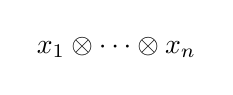
\begin{tikzpicture}[baseline={([yshift=-.5ex]current bounding box.center)}]
                \path coordinate[label=above:$x_1 \otimes \cdots \otimes x_n$] (a)
                +(1,0) coordinate (b);
                \LCOEV{a}{b}
            \end{tikzpicture}
        \end{align}
        \item 
        \begin{align}
            \bigl( \mathrm{ev}_a \circ (\varphi \otimes \psi),\, \mathrm{ev}_{a^*} \circ (\psi',\, \varphi')\bigr)
            &= \frac{(\varphi,\, \varphi')(\psi',\, \psi)}{\dim_p(a)}
        \end{align}
        \item $\forall a \in \mathrm{Simp}(\Cat{C})$ および $\forall \varphi \in \expval{x,\, a},\, \forall \varphi \in \expval{a^*,\, x^*},\, \forall \psi \in \expval{a^*,\, y},\; \forall \psi' \in \expval{y^*,\, a}$ に対して
        \begin{align}
            \begin{tikzpicture}[baseline={([yshift=-.5ex]current bounding box.center)}]
                \path coordinate (A)
                +(2,0) coordinate (f)
                +(3.5,0) coordinate (g)
                +(5.5,0) coordinate (B);
                \foreach \x in {-45,-15,15,45} {
                    \draw[-<-=.5] (A) to[out=\x,in={180-\x}] (f);
                    \draw[-<-=.5] (g) to[out=\x,in={180-\x}] (B);
                }
                \node[circlenode] at (f) {$\varphi_\bullet$};
                \node[circlenode] at (g) {$\varphi^\bullet$};
                \node[circle,fill=black!20,minimum size=10mm] at (A) {};
                \node[circle,fill=black!20,minimum size=10mm] at (B) {};
            \end{tikzpicture}
            = \begin{tikzpicture}[baseline={([yshift=-.5ex]current bounding box.center)}]
                \path coordinate (A)
                +(3,0) coordinate (B);
                \foreach \x in {-45,-15,15,45} {
                    \draw[-<-=.5] (A) to[out=\x,in={180-\x}] (B);
                }
                \node[circle,fill=black!20,minimum size=10mm] at (A) {};
                \node[circle,fill=black!20,minimum size=10mm] at (B) {};
            \end{tikzpicture}
        \end{align}
        
    \end{enumerate}
    
\end{mylem}

\begin{proof}
    \begin{enumerate}
        \item 左辺は $\Hom{\Cat{C}}(1,\, a \otimes a^*)$ の元だが,補題\ref{lem:rigid-hom}の同型 $\alpha^{-1}_{1,a,a} \colon \Hom{\Cat{C}} (1,\, a\otimes a^*) \xrightarrow{\cong} \Hom{\Cat{C}} (a,\, a) = \mathbb{K}$ から,ある定数 $A_a \in \mathbb{K}$ を用いて
        \begin{align}
            \alpha_{1,a,a}^{-1} \left(  \begin{tikzpicture}[baseline={([yshift=-.5ex]current bounding box.center)}]
                \path coordinate[bullet,label=below:$\varphi$] (f)
                +(-0.5,1.6) coordinate[label=left:$a$] (a)
                +(0.5,1) coordinate[label=left:$x$] (x)
                +(1.5,1) coordinate[label=right:$x^*$] (y)
                +(2.5,1.6) coordinate[label=right:$a^*$] (b)
                +(2,0) coordinate[bullet,label=below:$\psi$] (g);
                \REV{x}{y}
                \draw[->-=.5] (f) to[out=120,in=-90] (a);
                \draw[->-=.5] (f) to[out=60,in=-90] (x);
                \draw[-<-=.5] (g) to[out=120,in=-90] (y);
                \draw[-<-=.5] (g) to[out=60,in=-90] (b);
            \end{tikzpicture} \right) 
            &= A_a\quad 
            \begin{tikzpicture}[baseline={([yshift=-.5ex]current bounding box.center)}]
                \draw[->-=.5] (0,-1) -- node[midway,right] {$a$} (0,1);
            \end{tikzpicture}
        \end{align}
        が分かる.逆射 $a_{1,a,a}$ を作用させることで
        \begin{align}
            \begin{tikzpicture}[baseline={([yshift=-.5ex]current bounding box.center)}]
                \path coordinate[bullet,label=below:$\varphi$] (f)
                +(-0.5,1.6) coordinate[label=left:$a$] (a)
                +(0.5,1) coordinate[label=left:$x$] (x)
                +(1.5,1) coordinate[label=right:$x^*$] (y)
                +(2.5,1.6) coordinate[label=right:$a^*$] (b)
                +(2,0) coordinate[bullet,label=below:$\psi$] (g);
                \REV{x}{y}
                \draw[->-=.5] (f) to[out=120,in=-90] (a);
                \draw[->-=.5] (f) to[out=60,in=-90] (x);
                \draw[-<-=.5] (g) to[out=120,in=-90] (y);
                \draw[-<-=.5] (g) to[out=60,in=-90] (b);
            \end{tikzpicture}
            &= A_a \quad 
            \begin{tikzpicture}[baseline={([yshift=-.5ex]current bounding box.center)}]
                \path coordinate[label=left:$a$] (a)
                +(1,0) coordinate[label=right:$a^*$] (b);
                \LCOEV{a}{b}
            \end{tikzpicture}
        \end{align}
        が分かるので,両辺の\hyperref[def:qtrace]{量子トレース}を取ることで
        \begin{align}
            A_a = \frac{(\varphi,\, \psi)}{\dim_p(a)}
        \end{align}
        と求まる.
        \item $\Cat{C}$ が有限かつ半単純なので,$x \coloneqq x_1 \otimes \cdots \otimes x_n$ が単純対象である場合に示せば良い.(1) および $(\varphi_\alpha,\, \varphi^\beta) = \delta^\beta_\alpha$ を用いれば良い.
        \item (1) より明らか.
        \item $1 \in \mathrm{Simp}(\Cat{C})$ なので,(1) および $(\varphi_\alpha,\, \varphi^\beta) = \delta^\beta_\alpha$ を用いれば良い.
    \end{enumerate}
    
\end{proof}

\subsection{PL多様体に関する準備}

\begin{mydef}[label=def:PLmfd]{PL多様体}
    任意の座標変換が区分的線形であるようなアトラスを\textbf{PL構造} (piecewise linear structure) と呼び,区分的線形構造を持つ位相多様体を\textbf{PL多様体} (piecewise linear manifold) と呼ぶ.
\end{mydef}

2つの単体的複体 $K,\, L \in \Obj{\SimpSet}$ を取り,その幾何学的実現をそれぞれ $\abs{K},\, \abs{L}$ と書く.
\begin{itemize}
    \item 連続写像 $f \colon \abs{K} \lto \abs{L}$ が\textbf{PL写像}であるとは,$K,\, L$ の細分 $K',\, L'$ が存在して,$f$ が $K'$ の単体を $L'$ の単体に写し,各単体への制限が線型写像になっていることを言う.
    \item 同相写像 $f \colon \abs{K} \lto \abs{L}$ が\textbf{PL同相写像}であるとは,それがPL写像であることを言う.
    \item 勝手な単体 $A \in K$ に対し,
    \begin{align}
        \bm{\mathrm{St}(A)} &\coloneqq \bigl\{\, \sigma \in K \bigm| \sigma \cup A \in K \,\bigr\} \\
        \bm{\mathrm{Lk}(A)} &\coloneqq \bigl\{\, \sigma \in \mathrm{St}(A) \bigm| \sigma \cap A = \emptyset \,\bigr\} 
    \end{align}
    とおいてそれぞれ\textbf{星状複体} (star), \textbf{絡み複体} (link) と呼ぶ.
    \item 三角形分割された位相多様体 $(M,\, K,\, \psi \colon \abs{K} \xrightarrow{\approx} M)$ が\textbf{組み合わせ多様体} (combinatorial manifold) であるとは,$\forall v \in K_0$ に対して $\abs{\mathrm{Lk}(v)} \approx S^{\dim M - 1}$ が成り立つことを言う.
    また,位相多様体 $M$ を組み合わせ多様体にする三角形分割 $(K,\, \psi \colon \abs{K} \xrightarrow{\approx} M)$ のことを\textbf{組み合わせ三角形分割}と呼ぶ.
\end{itemize}

\begin{mytheo}[label=thm:PL-combinatorial]{}
    PL多様体は組み合わせ三角形分割を持つ.逆に,組み合わせ多様体はPL多様体である.
\end{mytheo}

定理\ref{thm:PL-combinatorial}により,以後PL多様体と組み合わせ多様体を区別しない.

\subsubsection{星状同値}

単体的複体 $K,\, L$ が,互いに頂点を1つも共有していないとする.このとき,これらの\textbf{join}と呼ばれる単体的複体を
\begin{align}
    \bm{K * L} \coloneqq \bigl\{\, \sigma \cup \tau \bigm| \sigma \in K \AND \tau \in L \,\bigr\} 
\end{align}
で定義する.また,$\forall \sigma \in K$ に対して
\begin{align}
    \bar{\sigma} &\coloneqq \bigl\{\, \tau \subset \sigma  \,\bigr\} , \\
    \partial\bar{\sigma} &\coloneqq \bigl\{\, \tau \subsetneq \sigma  \,\bigr\}
\end{align}
と定義する.

単体的複体 $K$ の\textbf{双星状移動} (bistellar move)\footnote{\textbf{Pachner move}とも言う.} とは,次のような操作のことを言う:
\begin{enumerate}
    \item まず,$\sigma \in K,\; \tau \notin K$ であって $\mathrm{Lk}_K (\sigma) = \partial \bar{\tau},\; \mathrm{St}_K (\sigma) = \bar{\sigma} * \bar{\tau}$ を充たすものを持ってくる.
    \item 次に,
    \begin{align}
        K \lmto \bigl(K \setminus (\bar{\sigma} * \partial \bar{\tau}) \bigr) \cup (\partial \bar{\sigma} * \bar{\tau})
    \end{align}
    なる置き換えをして新たな単体的複体を得る.
\end{enumerate}
2つの\hyperref[def:PLmfd]{PL多様体} $(M,\, K,\, \psi),\; (N,\, L,\, \varphi)$ が\textbf{双星状同値} (bistellar equivalent) であるとは,
$K$ に有限回の双星状移動を施すことで $L$ にすることができること.

\begin{mytheo}[label=thm:Pachner]{Pachnerの定理}
    PL同相 $\IFF$ 双星状同値
\end{mytheo}

従って,PL多様体の上に構成した量が位相不変量(i.e. PL不変量)であることを示すには,それが双星状移動に関して不変であることを示すだけで良い.

\subsubsection{多面体分割}

技術的な理由により,\textbf{多面体分割} (polytope decomposition) を導入する~\cite[p.11]{KirillovBalsam2010TVBW}.

\begin{mydef}[label=def:polyhedron,breakable]{2-多面体}
    \begin{itemize}
        \item 2次元コンパクト多様体\footnote{位相多様体.境界はついていてもいなくても良い.} $P$ が\textbf{2-多面体} (2-polyhedra) であるとは,$P$ の三角形分割 $\psi \colon \abs{K} \xrightarrow{\approx} P$ であって,任意の0-単体および1単体がある2-単体の面になっているものが存在することを言う.
        \item 2-多面体の\textbf{層状化} (stratification) とは,$P$ に埋め込まれたグラフ\footnote{ここでは,位相空間としてのグラフを考えている.} $P^{(1)} \subset P$ であって $P \setminus \Int(P) \subset P^{(1)}$
        \textbf{層状化された多面体} (stratified polyhedra) とは,2-多面体 $P$ とその層状化 $P^{(1)} \subset P$ の組み $(P,\, P^{(1)})$ のこと.
        \begin{figure}[H]
            \centering
            \begin{tikzpicture}
                \path coordinate (a)
                ++(2,0) coordinate (b)
                ++(0.4,2) coordinate (c)
                ++(-1.6,1) coordinate (d)
                ++(-1,-1.2) coordinate (e);
                \coordinate (g) at (barycentric cs:a=1,b=1,c=1,d=1,e=1);
                \coordinate (l) at (barycentric cs:b=1,c=1,g=1);
                \coordinate (p) at (barycentric cs:c=1,d=1);
                \coordinate (m) at ($(c) + (0.5,0.5)$);
                \node at (l) {$P$};
                \node[red,right] at (m) {$P^{(1)}$};
                \draw[red,->] (m) to[out=180,in=60] (p);
                \draw[spath/save=bdy] (a) -- (b) -- (c) -- (d) -- (e) -- cycle;
                \draw[red,thick,spath/use=bdy];
                \draw[red,thick] (g) -- (a);
                \draw[red,thick] (g) -- (b);
                \draw[red,thick] (g) -- (c);
                \draw[red,thick] (g) -- (d);
                % \draw[red,thick] (g) -- (e);
                \begin{scope}[on background layer]
                    \fill[gray!20, spath/use=bdy];
                \end{scope}
            \end{tikzpicture}
            \caption{層状化された多面体 $(P,\, P^{(1)})$}
        \end{figure}%        
        \item 層状化された多面体 $(P,\, P^{(1)})$ において,$P \setminus P^{(1)}$ の連結成分の閉包を\textbf{領域} (region) と呼ぶ.$(P,\, P^{(1)})$ の領域を全て集めた集合を $\mathrm{Reg}(P)$ と書くことにする.
        
         領域 $R \in \mathrm{Reg}(P)$ が\textbf{埋め込み可能}であるとは,全射 $p \colon \partial(\overline{P \setminus P^{(1)}}) \twoheadrightarrow P^{(1)}$ の制限 $p|_{\partial R} \colon \partial R \to P^{(1)}$ が単射であることを言う.
        \item 層状化された多面体 $(P,\, P^{(1)})$ において,
        頂点 $v \in \mathsf{V}(P^{(1)})$ の\textbf{分岐}とは,連続曲線 $\gamma \colon [0,\, 1] \lto P$ であって $\gamma (0) = v$ かつ $\gamma \bigl( (0,\, 1] \bigr) \subset P \setminus P^{(1)}$ を充たすもののホモトピー類のこと.
        頂点 $v$ の分岐の総数を,頂点 $v$ の\textbf{配位数} (valence) と呼ぶ.
        \item 層状化された多面体 $(P,\, P^{(1)})$ において,
        辺 $e \in \mathsf{E}(P^{(1)})$ の\textbf{分岐}とは,連続曲線 $\gamma \colon [0,\, 1] \lto P$ であって $\gamma (0) \in \Int(e)$ かつ $\gamma \bigl( (0,\, 1] \bigr) \subset P \setminus P^{(1)}$ を充たすもののホモトピー類のこと.
        辺 $e$ の分岐がなす集合を $P^{(1)}_e$ と書き,$\abs{P^{(1)}_e} \in \mathbb{N}$ を辺 $e$ の\textbf{配位数} (valence) と呼ぶ.
        \item 層状化された多面体 $(P,\, P^{(1)})$ の\textbf{向き} (orientation) とは,位相空間 $P \setminus P^{(1)}$ の向きのこと.
        \begin{figure}[H]
            \centering
            \begin{tikzpicture}
                \path coordinate (a)
                ++(2,0) coordinate (b)
                ++(0.4,2) coordinate (c)
                ++(-1.6,1) coordinate (d)
                ++(-1,-1.2) coordinate (e);
                \coordinate (g) at (barycentric cs:a=1,b=1,c=1,d=1,e=1);
                \coordinate (P) at (barycentric cs:a=1,b=1,g=1);
                \coordinate (Q) at (barycentric cs:b=1,c=1,g=1);
                \coordinate (R) at (barycentric cs:c=1,d=1,g=1);
                \coordinate (S) at (barycentric cs:d=1,e=1,a=1,g=1);

                \draw[spath/save=bdy] (a) -- (b) -- (c) -- (d) -- (e) -- cycle;
                \draw[red,thick,spath/use=bdy];
                \draw[red,thick] (g) -- (a);
                \draw[red,thick] (g) -- (b);
                \draw[red,thick] (g) -- (c);
                \draw[red,thick] (g) -- (d);
                % \draw[red,thick] (g) -- (e);

                \draw[->] ($(P)+(0.2,0)$) arc (0:270:0.2);
                \draw[->] ($(Q)+(0.2,0)$) arc (0:-270:0.2);
                \draw[->] ($(R)+(0.2,0)$) arc (0:270:0.2);
                \draw[->] ($(S)+(0.2,0)$) arc (0:-270:0.2);
                \begin{scope}[on background layer]
                    \fill[gray!20, spath/use=bdy];
                \end{scope}
            \end{tikzpicture}
            \caption{層状化された多面体の向き}
        \end{figure}%
    \end{itemize}
    
\end{mydef}

\begin{mydef}[label=def:graph-bdy]{境界グラフ}
    \begin{itemize}
        \item \hyperref[def:polyhedron]{層状化された多面体} $(P,\, P^{(1)})$ の\textbf{境界} (boundary) とは,グラフ
        \begin{align}
            \partial P \coloneqq \bigl\{\, e \in \mathsf{E}(P^{(1)}) \bigm| \text{配位数}\;1 \,\bigr\} 
        \end{align}
        のこと.$(P,\, P^{(1)})$ の向きは,グラフ $\partial P$ に向きを誘導する.
        \item \hyperref[def:polyhedron]{層状化された多面体} $(P,\, P^{(1)})$ が\textbf{円筒境界を持つ}とは,
        $\forall v \in \mathsf{V}(\partial P)$ に対して $e_v \in \mathsf{E}(P^{(1)}) \setminus \mathsf{E}(P^{(1)})$ がただ1つ存在し,以下を充たすことを言う:
        \begin{itemize}
            \item $d_v$ の端点のうち1つは $v$ で,もう1つは $v$ でない.
            \item $v$ の全ての分岐に隣接する
        \end{itemize}
        このとき,位相多様体 $\partial P \subset P$ は $\partial P \times [0,\, 1]$ と同相な近傍を持つ.
    \end{itemize}
\end{mydef}

位相空間
\begin{align}
    \mathcal{B} \coloneqq \bigl\{\, (x^1,\, x^2,\, x^3) \in \mathbb{R}^3 \bigm| x^3 = 0 \,\bigr\} \cup \bigl\{\, (x^1,\, x^2,\, x^3) \in \mathbb{R}^3 \bigm| x^1 = 0,\, x^3 > 0 \,\bigr\} \cup \bigl\{\, (x^1,\, x^2,\, x^3) \in \mathbb{R}^3 \bigm| x^2 = 0,\, x^3 < 0 \,\bigr\} 
\end{align}
を考える.図示すると次のようになる:
\begin{figure}[H]
    \centering
    \begin{tikzpicture}
        \path coordinate[bullet] (O)
        +(2,0) coordinate (xr)
        +(2,-2) coordinate (xrd)
        +(-2,0) coordinate (xl)
        +(-2,-2) coordinate (xld)
        +(0.4,0.5) coordinate (yr)
        +(0.4,2.5) coordinate (yru)
        +(-0.4,-0.5) coordinate (yl)
        +(-0.4,1.5) coordinate (ylu);

        \draw (xl) -- (xr) -- (xrd) -- (xld) --cycle;
        \draw (yl) -- (yr) -- (yru) -- (ylu) -- cycle;
        \draw (yl) -- ++(2,0) -- ++(0.8,1) -- (yr) -- cycle;
        \draw (yr) -- ++(-2,0) -- ++(-0.8,-1) -- (yl) -- cycle;

        \draw[->] (xl) -- (2.5,0) node[right] {$x^1$};
        \draw[->] (yl) -- ($(yr)+(0.5,0.625)$) node[above right] {$x^2$};
        \draw[->] (O.center) -- ++(0,2.5) node[above] {$x^3$};
    \end{tikzpicture}    
    \caption{位相空間 $\mathcal{B}$}
\end{figure}%

\begin{mydef}[label=def:polyhedra-special]{2-多面体のクラス}
    \begin{itemize}
        \item \hyperref[def:polyhedron]{層状化された多面体} $(P,\, P^{(1)})$ が\textbf{正則} (regular) であるとは,$P$ の部分空間 $\forall R \in \mathrm{Reg}(P)$ が $R \approx D^2$ でかつ\hyperref[def:polyhedron]{埋め込み可能}であることを言う.
        \item \hyperref[def:polyhedron]{層状化された多面体} $(P,\, P^{(1)})$ が\textbf{特殊} (special) であるとは,以下の条件を充たすことを言う:
        \begin{enumerate}
            \item $\forall p \in P$ に対してある開近傍 $p \in U \subset P$ および開部分集合 $V \subset \mathcal{B}$ が存在し,$U \approx V$ となる.
            \item $P$ の各連結成分には,(1) の同相写像で $\mathcal{B}$ の原点に移されるような点が少なくとも1つ存在する.
            \item $P \setminus \Int(P)$ の各連結成分は $S^1$ と同相でない.
        \end{enumerate}
        
    \end{itemize}
    
\end{mydef}

\begin{myexample}[label=ex:tetrahedron]{4面体の重心細分}
    4面体の重心細分として得られる\hyperref[def:polyhedra-special]{層状化された多面体}は,正則かつ特殊である.
\end{myexample}


\begin{mydef}[label=def:polytope-decomp]{多面体分割}
    向き付けられた $3$ 次元閉多様体 $M$ の\textbf{多面体分割}とは,\hyperref[def:graph-bdy]{境界グラフ}が空の\footnote{従って,$\forall e \in \mathsf{E}(P^{(1)})$ の配位数は2以上である.}\hyperref[def:polyhedron]{向き付けられ,層状化された多面体} $(P,\, P^{(1)})$ であって,
    $M$ に埋め込まれており,$M \setminus P$ が開球のdisjoint unionになっているもののこと. 
    % \begin{itemize}
    %     \item $3$ 次元閉多様体 $M$ の多面体分割 $(P,\, P^{(1)})$ が\textbf{正則} (regular) であるとは,層状化された多面体 $(P,\, P^{(1)})$ が\hyperref[def:polyhedra-special]{正則}であることを言う.
    %     \item $3$ 次元閉多様体 $M$ の多面体分割 $(P,\, P^{(1)})$ が\textbf{特殊} (special) であるとは,層状化された多面体 $(P,\, P^{(1)})$ が\hyperref[def:polyhedra-special]{特殊}であることを言う.
    % \end{itemize}
    
    \tcblower

    向き付けられた境界付き $3$ 次元コンパクト多様体 $M$,およびその境界に埋め込まれた有向グラフ $G \subset \partial M$ を与える.$\forall v \in \mathsf{V}(G)$ の\hyperref[def:polyhedron]{配位数}は2以上であるとする\footnote{従って,境界の境界は考えない.}.
    組 $(M,\, G)$ の\textbf{多面体分割}とは,\hyperref[def:graph-bdy]{$\partial$-円筒境界を持つ},\hyperref[def:polyhedron]{向き付けられ,層状化された2-多面体} $(P\, P^{(1)})$ であって,
    \begin{enumerate}
        \item $P$ は $M$ に埋め込まれている
        \item 有向グラフとして $\partial P = G$ で,かつ $P \setminus \partial P \subset M \setminus \partial M$
        \item $M \setminus P$ は3-開球および3次元多様体 $(\partial M \setminus G) \times [0,\, 1)$ のdisjoint unionである.
    \end{enumerate}
    
\end{mydef}

$M$ の多面体分割 $(P,\, P^{(1)})$ の任意の頂点 $v \in \mathsf{V}(P^{(1)})$ に対して,$v$ の閉球近傍 $B_v \subset M$ を十分小さく取ることで図のようなグラフを得る:
これを頂点 $v$ の\textbf{絡みグラフ}と呼び,$\mathrm{Lk}(v)$ と書くことにする.

\begin{mytheo}[label=thm:MP-polytope,breakable]{多面体分割のPL不変性}
    向き付けられた境界付き $3$ 次元コンパクト多様体 $M$,およびその境界に埋め込まれた有向グラフ $G \subset \partial M$ を与える.$\forall v \in \mathsf{V}(G)$ の\hyperref[def:polyhedron]{配位数}は2以上であるとする\footnote{従って,境界の境界は考えない.}.

    このとき,$(M,\, G)$ の任意の2つの\hyperref[def:polytope-decomp]{多面体分割} $(P,\, P^{(1)}),\, (P',\, P'{}^{(1)})$ は,以下の操作の有限回の組み合わせで互いに写り合う:
    \begin{description}
        \item[\textbf{(T0)}] $\partial D^2 = D^2 \cap P \subset P \setminus P^{(1)}$ を充たすような2次元円板 $D^2$ を $P$ に付け足す.さらにグラフ $P^{(1)}$ に1つの頂点とループ辺 $\partial D^2$ を付け足す.
        \begin{align}
            T_0 \colon
            \begin{tikzpicture}[baseline={([yshift=-.5ex]current bounding box.center)}]
                \path coordinate (a)
                ++(2,0) coordinate (b)
                ++(0.5,1.5) coordinate (c)
                ++(-2,0) coordinate (d);
                \draw[dashed,spath/save=frame] (a) to[out=-10,in=-170] (b) to[out=30,in=-60] (c) to[out=170,in=10] (d) to[out=-150,in=120] (a);
                \begin{scope}[on background layer]
                    \fill[gray!20, spath/use=frame];
                \end{scope}
            \end{tikzpicture}
            \lmto 
            \begin{tikzpicture}[baseline={([yshift=-.5ex]current bounding box.center)}]
                \path coordinate (a)
                ++(2,0) coordinate (b)
                ++(0.5,1.5) coordinate (c)
                ++(-2,0) coordinate (d);
                \coordinate (g) at (barycentric cs:a=1,b=1,c=1,d=1);
                \draw[dashed,spath/save=frame] (a) to[out=-10,in=-170] (b) to[out=30,in=-60] (c) to[out=170,in=10] (d) to[out=-150,in=120] (a);
                \draw[spath/save=bubble] ($(g)+(-0.8,0)$) to[out=90,in=90] ($(g)+(0.8,0)$) arc (0:-180:0.8 and 0.2);
                \draw[red,thick] ($(g)+(0.8,0)$) arc (0:360:0.8 and 0.2);
                \node[bullet,red] at ($(g) + (0,-0.2)$) {};
                \begin{scope}[on background layer]
                    \fill[gray!20, spath/use=frame];
                    \fill[red!20, spath/use=bubble];
                \end{scope}
            \end{tikzpicture}
        \end{align}
        
        \item[\textbf{(T1)}] 
        
        \begin{align}
            T_1 \colon
            \begin{tikzpicture}[baseline={([yshift=-.5ex]current bounding box.center)}]
                \path coordinate (a)
                ++(2,0) coordinate (b)
                ++(0.5,1.5) coordinate (c)
                ++(-2,0) coordinate (d);
                \coordinate (g) at (barycentric cs:a=1,b=1,c=1,d=1);
                \coordinate[bullet] (p) at ($(g) + (-0.5,0)$);
                \coordinate[bullet] (q) at ($(g) + (0.5,0)$);
                \draw[dashed,spath/save=frame] (a) to[out=-10,in=-170] (b) to[out=30,in=-60] (c) to[out=170,in=10] (d) to[out=-150,in=120] (a);
                \clip[spath/use=frame];
                \draw (p) -- ++(120:2);
                \draw (p) -- ++(180:2);
                \draw (p) -- ++(-120:2);
                \draw (q) -- ++(60:2);
                \draw (q) -- ++(0:2);
                \draw (q) -- ++(-60:2);
                \begin{scope}[on background layer]
                    \fill[gray!20, spath/use=frame];
                \end{scope}
            \end{tikzpicture}
            \lmto 
            \begin{tikzpicture}[baseline={([yshift=-.5ex]current bounding box.center)}]
                \path coordinate (a)
                ++(2,0) coordinate (b)
                ++(0.5,1.5) coordinate (c)
                ++(-2,0) coordinate (d);
                \coordinate (g) at (barycentric cs:a=1,b=1,c=1,d=1);
                \coordinate[bullet] (p) at ($(g) + (-0.5,0)$);
                \coordinate[bullet] (q) at ($(g) + (0.5,0)$);
                \draw[thick,red] (p) -- (q);
                \draw[dashed,spath/save=frame] (a) to[out=-10,in=-170] (b) to[out=30,in=-60] (c) to[out=170,in=10] (d) to[out=-150,in=120] (a);
                \clip[spath/use=frame];
                \draw (p) -- ++(120:2);
                \draw (p) -- ++(180:2);
                \draw (p) -- ++(-120:2);
                \draw (q) -- ++(60:2);
                \draw (q) -- ++(0:2);
                \draw (q) -- ++(-60:2);
                \begin{scope}[on background layer]
                    \fill[gray!20, spath/use=frame];
                \end{scope}
            \end{tikzpicture}
        \end{align}

        \item[\textbf{(T2)}] 
  
        \begin{align}
            T_2 \colon
            \begin{tikzpicture}[baseline={([yshift=-.5ex]current bounding box.center)}]
                \path coordinate (a)
                ++(2,0) coordinate (b)
                ++(0.5,1.5) coordinate (c)
                ++(-2,0) coordinate (d);
                \coordinate (g) at (barycentric cs:a=1,b=1,c=1,d=1);
                \coordinate[bullet] (p) at ($(g) + (-0.5,0)$);
                \coordinate[bullet] (q) at ($(g) + (0.5,0)$);
                \draw[dashed,spath/save=frame] (a) to[out=-10,in=-170] (b) to[out=30,in=-60] (c) to[out=170,in=10] (d) to[out=-150,in=120] (a);
                \clip[spath/use=frame];
                \draw (p) -- (q);
                \draw (p) -- ++(120:2);
                \draw (p) -- ++(180:2);
                \draw (p) -- ++(-120:2);
                \draw (q) -- ++(60:2);
                \draw (q) -- ++(0:2);
                \draw (q) -- ++(-60:2);
                \begin{scope}[on background layer]
                    \fill[gray!20, spath/use=frame];
                \end{scope}
            \end{tikzpicture}
            \lmto 
            \begin{tikzpicture}[baseline={([yshift=-.5ex]current bounding box.center)}]
                \path coordinate (a)
                ++(2,0) coordinate (b)
                ++(0.5,1.5) coordinate (c)
                ++(-2,0) coordinate (d);
                \coordinate[bullet] (g) at (barycentric cs:a=1,b=1,c=1,d=1);
                \draw[dashed,spath/save=frame] (a) to[out=-10,in=-170] (b) to[out=30,in=-60] (c) to[out=170,in=10] (d) to[out=-150,in=120] (a);
                \clip[spath/use=frame];
                \draw (g) -- ++(120:2);
                \draw (g) -- ++(180:2);
                \draw (g) -- ++(-120:2);
                \draw (g) -- ++(60:2);
                \draw (g) -- ++(0:2);
                \draw (g) -- ++(-60:2);
                \begin{scope}[on background layer]
                    \fill[gray!20, spath/use=frame];
                \end{scope}
            \end{tikzpicture}
        \end{align}

 
        \item[\textbf{(T3)}] 
        
        \begin{align}
            T_3 \colon
            \begin{tikzpicture}[baseline={([yshift=-.5ex]current bounding box.center)}]
                \path coordinate (a)
                ++(2,0) coordinate (b)
                ++(0.5,1.5) coordinate (c)
                ++(-2,0) coordinate (d);
                \coordinate[bullet] (g) at (barycentric cs:a=1,b=1,c=1,d=1);
                \draw[dashed,spath/save=frame] (a) to[out=-10,in=-170] (b) to[out=30,in=-60] (c) to[out=170,in=10] (d) to[out=-150,in=120] (a);
                \clip[spath/use=frame];
                \draw (g.center) -- ++(30:2);
                \draw (g.center) to[out=90,in=-90] ++(150:2);
                \draw (g.center) to[out=-120,in=90] ++(-150:2);
                \draw (g.center) -- ++(-30:2);
                \begin{scope}[on background layer]
                    \fill[gray!20, spath/use=frame];
                \end{scope}
            \end{tikzpicture}
            \lmto 
            \begin{tikzpicture}[baseline={([yshift=-.5ex]current bounding box.center)}]
                \path coordinate (a)
                ++(2,0) coordinate (b)
                ++(0.5,1.5) coordinate (c)
                ++(-2,0) coordinate (d);
                \coordinate[bullet] (g) at (barycentric cs:a=1,b=1,c=1,d=1);
                \draw[dashed,spath/save=frame] (a) to[out=-10,in=-170] (b) to[out=30,in=-60] (c) to[out=170,in=10] (d) to[out=-150,in=120] (a);
                \clip[spath/use=frame];
                \draw (g.center) -- ++(30:2);
                \draw (g.center) to[out=90,in=-90] ++(150:2);
                \draw (g.center) to[out=-120,in=90] ++(-150:2);
                \draw (g.center) -- ++(-30:2);
                \draw[spath/save=reg] ($(g)+(-0.8,0)$) to[out=90,in=180] ($(g) + (-0.2,0.6)$) to[out=0,in=180] ($(g) + (0.2,0.4)$) to[out=0,in=-150] ($(g) + (30:2)$);
                \draw[red,thick] (g) arc (0:360:0.4 and 0.1);
                \begin{scope}[on background layer]
                    \fill[gray!20, spath/use=frame];
                    \clip[spath/use=frame];
                    \fill[red!20, spath/use=reg] -- ($(g) + (-30:2)$) -- (g) arc(0:-180:0.4 and 0.1);
                \end{scope}
            \end{tikzpicture}
        \end{align}
    \end{description}
    
\end{mytheo}

\begin{proof}
    ~\cite[Theorem 11.5, p.250]{Turaev2017}
\end{proof}


% \begin{mydef}[label=def:polytope-decomp]{多面体分割}
%     $d = 2,\, 3$ 次元の\hyperref[def:PLmfd]{PL多様体} $(M,\, K,\, \psi)$ の\textbf{多面体分割} (polytope decomposition) とは,三角形分割 $\psi \colon \abs{K} \xrightarrow{\approx} M$ に以下の操作を施して得られる $M$ の胞体分割のこと:
%     \begin{description}
%         \item[\textbf{(M1)}] 
%         \item[\textbf{(M2)}] 
%         \item[\textbf{(M3)}] 
%     \end{description}
% \end{mydef}

% \begin{mytheo}[label=thm:polytope]{多面体分割のPL不変性}
%     3次元の境界付き\hyperref[def:PLmfd]{PL多様体} $M$ および2次元境界付き部分多様体 $X \subset \partial M$ を与える.
%     $\mathcal{N}$ を $X$ の\hyperref[def:polytope-decomp]{多面体分割}とするとき,以下が成り立つ:
%     \begin{enumerate}
%         \item $\mathcal{N}$ は $M$ の多面体分割 $\mathcal{M}$ へ拡張することができる.
%         \item $M$ の任意の2つの多面体分割 $\mathcal{M}_1,\, \mathcal{M}_2$ であって,$\mathcal{M}_1|_{X} = \mathcal{M}_2|_X = \mathcal{N}$ を充たすものは,有限回の\textsf{\textbf{(M1)-(M3)}}の操作によって $\mathcal{N}$ を変えることなく互いに写り合う.
%     \end{enumerate}
%     % の任意の2つの\hyperref[def:polytope-decomp]{多面体分割}は,有限回の\textsf{\textbf{(M1)-(M3)}}の操作によって互いに写り合う.
% \end{mytheo}

% \begin{proof}
    
% \end{proof}

\subsection{グラフ上のアイソトピー不変量}



\subsection{Turaev-Viro不変量の構成}

\subsubsection{閉多様体の場合}

向き付けられた3次元閉多様体 $M$ の\hyperref[def:polytope-decomp]{多面体分割} $(P,\, P^{(1)})$ をとる.
$P$ の\textbf{彩色} (coloring) とは,
写像
\begin{align}
    c \colon \mathrm{Reg}(P) \lto \Simp(\Cat{C})
\end{align}
のこと.ここで,
\begin{align}
    \dim (c) \coloneqq \prod_{R \in \mathrm{Reg}(P)} \bigl( \dim_p \bigl( c(R) \bigr)  \bigr)^{\chi(R)} \in \mathbb{K}
\end{align}
と定義する.ただし $\chi(R)$ は $R$ のEuler標数である.

彩色 $c \colon \mathrm{Reg}(P)$ を1つ固定したとき,対応する $Z(c;\, P) \in \mathbb{K}$ を構成しよう.
まず $\mathsf{V}(P^{(1)}) = \empty$ のときは $\abs{c} \coloneqq 1$ と定義する.
$\mathsf{V}(P^{(1)}) \neq \empty$ の場合を考える.
$\forall e \in \mathsf{E}(P^{(1)})$ に勝手な向きを与える.
すると,辺 $e$ の\hyperref[def:polyhedron]{分岐}の集合 $P^{(1)}_e$ にはサイクリックな順序を入れることができる.
さらに $\forall b \in P_e^{(1)}$ に対して,$\epsilon_b \in \{\pm\}$ を $M$ から誘導される向きと $e$ の向きが整合しているならば $+$,不整合ならば $-$ となるように定義することで,
\begin{align}
    \mathcal{H}(e;\, c) \coloneqq \expval{c(b_1)^{\epsilon_{b_1}},\, \dots,\, c(b_n)^{\epsilon_{b_n}}} \WHERE P_e^{(1)} = \{b_1 < \cdots < b_n\}
\end{align}
と構成しよう.補題\ref{lem:MS}の\textsf{\textbf{(Rotation isomorphism)}} により $\mathcal{H}(e;\, c)$ はwell-definedである.
\begin{align}
    \mathcal{H}(c) \coloneqq \bigotimes_{e \in \mathsf{E}(P^{(1)})} \mathcal{H}(e;\, c)
\end{align}
とおく.

$\forall v \in \mathsf{V}(P^{(1)})$ に対しては,まずそれの絡み近傍 $B_v$ および絡みグラフ $\mathrm{Lk}(v) \subset B_v$ をとる.
$\partial B_v$ には $M$ から誘導される向きを入れる.$\forall a \in \mathsf{E}\bigl(\mathrm{Lk}(v)\bigr)$ はある1つの\hyperref[def:polyhedron]{領域} $R_a$ に含まれているから,$a$ には $c(R_a) \in \Simp(\Cat{C})$ を割り当て,$a$ 自身の向きとしては $R_a \setminus \Int(B_a)$ から誘導されるものを入れる.
ここで,$\forall x \in \mathsf{V}\bigl(\mathrm{Lk}(v)\bigr)$ に対して勝手な $\alpha_x \in \expval{c(a_1)^{\epsilon_{a_1}},\, \dots,\, c(a_m)^{\epsilon_{a_m}}}$ を割り当てることで,絡みグラフ $\mathrm{Lk}(v) \subset B_v$ をストリング図式に読み替える.特に $M$ が境界を持たないことから絡みグラフは配位数が $2$ 以上なので,このようにして得られたストリング図式は端点を持たない.
i.e. ストリング図式に対応する射は $\mathbb{F}_{\Cat{C}} \bigl( \mathrm{Lk}(v) \bigr)\bigl( \bigotimes_{x \in \mathsf{V} \bigl( \mathrm{Lk}(v) \bigr) } \alpha_x \bigr) \in \Hom{\Cat{C}} (1,\, 1)$ と書ける.これを $\mathbb{K}$-線形に拡張することで
,$\mathbb{K}$-線型写像
\begin{align}
    \mathbb{F}_{\Cat{C}} \bigl( \mathrm{Lk}(v) \bigr) \in \Hom{\VEC{\mathbb{K}}} \left( \mathcal{H}(\mathrm{Lk}(v)),\, \mathbb{K}\right) 
\end{align}
を得る.ここで
\begin{align}
    \mathcal{H}(\mathrm{Lk}(v)) \cong \bigotimes_{e_v;\, v\, \text{を端点に持つ}} \mathcal{H}(e_v;\, c)
\end{align}
より
\begin{align}
    \bigotimes_{v \in \mathsf{V}(P^{(1)})}\Hom{\VEC{\mathbb{K}}} \left( \mathcal{H}(\mathrm{Lk}(v)),\, \mathbb{K}\right)  
    &\cong \bigotimes_{v} \bigotimes_{e_v;\, v\, \text{を端点に持つ}} \Hom{\VEC{\mathbb{K}}} \left( \mathcal{H}(e_v;\, c),\, \mathbb{K}\right) \\
    &\cong \Hom{\VEC{\mathbb{K}}} \bigl(H(c),\, \mathbb{K}\bigr)
\end{align}
であるから,
\begin{align}
    \bigotimes_{v}\mathbb{F}_{\Cat{C}} \bigl( \mathrm{Lk}(v) \bigr) \in \Hom{\VEC{\mathbb{K}}} \bigl(H(c),\, \mathbb{K}\bigr)
\end{align}
がわかる.



% \hyperref[def:polytope-decomp]{多面体分割}された\hyperref[def:PLmfd]{PL多様体} $(M,\, \mathcal{M},\, \psi)$ を与える.$\mathcal{M}$ の全ての辺 $e \in \mathcal{M}_1$ に向き $\epsilon_e \in \{\pm 1\}$ を与え\footnote{この向きは,大元の三角形分割から誘導されるものである},それを $\mathcal{O} \coloneqq \Familyset[\big]{\epsilon_e}{e \in \mathcal{M}_1}$ と書く.
% 向き付けられた多面体分割を $\mathcal{M}^{\mathcal{O}}$ と書く.

% \begin{mydef}[label=def:state]{状態}
%     \textbf{状態} (state) とは,写像
%     \begin{align}
%         \Gamma \colon \mathcal{M}^{\mathcal{O}}_1 \lto \Obj{\Cat{C}}
%     \end{align}
%     であって
%     \begin{align}
%         \Gamma(-e) = \Gamma(e)^*
%     \end{align}
%     を充たすもののこと.
%     \tcblower
%     2つの状態 $\Gamma_1,\, \Gamma_2$ が同値であるとは,$\forall e \in \mathcal{M}^{\mathcal{O}}_1$ に対して $\Gamma_1(e) \cong \Gamma_2(e)$ が成り立つこと.
% \end{mydef}

% \hyperref[def:state]{状態} $\Gamma \colon \mathcal{M}^{\mathcal{O}}_1 \lto \Obj{\Cat{C}}$ を1つ固定する.このときの\textbf{状態空間} (state space) とは,写像
% \begin{align}
%     \mathcal{H} (\mhyphen;\, \Gamma) \colon \mathcal{M}^{\mathcal{O}}_2 &\lto \Obj{\Vec{\mathbb{K}}}, \\
%     \sigma &\lmto  \expval{\Gamma(e_1),\, \dots,\, \Gamma(e_n)} \WHERE \partial \sigma = e_1 \cup \cdots \cup e_n
% \end{align}
% ただし,$e_1,\, \cdots ,\, e_n$ は $\sigma$ の向きから誘導される向きに辿る.なお,\hyperref[lem:MS]{\textsf{\textbf{(Rotation isomorphism)}}}により始点をどこにとっても良いことには注意する.
% 最後に,任意の2次元組み合わせ部分多様体 $N \subset M,\; \mathcal{N}^{\mathcal{o}} \subset \mathcal{M}_2^{\mathcal{O}}$ について
% \begin{align}
%     \mathcal{H}(N) \coloneqq \bigoplus_{\Gamma \colon \mathcal{M}^{\mathcal{O}}_1 \lto \Obj{\Cat{C}}} \mathcal{H}(N;\, \Gamma)
% \end{align}
% と定義することで,Hilbert空間の構成が完了する.特に補題\ref{lem:nondegen-pairing}より
% \begin{align}
%     \label{eq:TVBW-involutive}
%     \mathcal{H}(-N) = \mathcal{H}(N)^*
% \end{align}
% が成り立つ.

% 次に,3次元多様体 $M$ 自身の分配関数を構成する.
% そのためにはまず\hyperref[def:state]{状態} $\Gamma \colon \mathcal{M}^{\mathcal{O}}_1 \lto \Obj{\Cat{C}}$ を1つ固定し,任意の3-セル $\mu \in \mathcal{M}^{\mathcal{O}}_3$ に対して,上手い位相不変量
% \begin{align}
%     Z(\mu;\, \Gamma) \in \mathcal{H} (\partial\mu;\, \Gamma) = \bigotimes_{\sigma \in \{\partial\mu\;\text{の面}\}} \expval{\Gamma(\partial\sigma_1),\, \dots,\, \Gamma(\partial\sigma_n)}
% \end{align}
% を見つけてくる必要がある.
% そこで,些か天下り的だが,$\partial\mu$ の辺のPoincar\'{e}双対のグラフ $\mu^{\vee}$ をとり,
% \begin{itemize}
%     \item 辺には $\Gamma(e)^{\pm} \in \Obj{\Cat{C}}$ を
%     \item 頂点(ちょうど $\partial\mu$ の面の個数だけ存在する)には $\varphi_\sigma \in \expval{\Gamma(e_1)^{\pm},\, \cdots,\, \Gamma(e_n)^{\pm}} \WHERE \partial\sigma = e_1 \cup \cdots \cup e_n$ を
% \end{itemize}
% 載せる.このようなとき,後述する方法により\textbf{Reshetikhin-Turaev不変量} $\irm{Z}{RT}(\mu^{\vee};\, \Gamma,\, \{\varphi_\sigma\}) \in \mathbb{K}$ を構成することができる.

% 補題\ref{lem:nondegen-pairing}の2次形式は非退化だから,結局
% \begin{align}
%     \bigl( Z(\mu;\, \Gamma),\, \bigotimes_{\sigma \in \{\partial\mu\;\text{の面}\}} \varphi_\sigma \bigr) \coloneqq \irm{Z}{RT}(\mu^{\vee};\, \Gamma,\, \{\varphi_\sigma\})
% \end{align}
% によって $Z(\mu;\, \Gamma) \in \mathcal{H} (\partial\mu;\, \Gamma)$ を定義できる.

% \begin{mydef}[label=def:inv-TV]{Turaev-Viro不変量}
%     \hyperref[def:polytope-decomp]{多面体分割}された境界付き3次元\hyperref[def:PLmfd]{PL多様体} $(M,\, \mathcal{M},\, \psi)$ を与える.
%     このとき,\textbf{Turaev-Viro不変量}を以下のように定義する:
%     \footnotesize
%     \begin{align}
%         \irm{Z}{TV}(M) \coloneqq \left( \sum_{a \in \mathrm{Simp}(\Cat{C})} \dim(a)^2\right)^{-v(M)} \sum_{\Gamma \colon \mathcal{M}^{\mathcal{o}}_1 \to \Obj{\Cat{C}}} \left( \lev \left( \bigotimes_{\mu \in \mathcal{M}^{\mathcal{O}}_3} Z(\mu;\, \Gamma) \right) \prod_{e \in \mathcal{M}_1} \dim \bigl( \Gamma(e) \bigr) ^{n_e}  \right)
%     \end{align}
%     \normalsize
%     ただし,
%     \begin{align}
%         v(M) &\coloneqq \#\{\text{vertex in}\; \mathrm{Int}(M)\} + \frac{1}{2} \# \{\text{vertex on}\; \partial M\} \\
%         n_e &\coloneqq \begin{cases}
%             1, & e \in \mathrm{Int}(M) \\
%             1/2, & e \in \partial M
%         \end{cases}
%     \end{align}
%     とおいた.
% \end{mydef}


% \begin{mytheo}[label=thm:TVBW]{}
%     $\irm{Z}{TV}(M)$ は $M$ の\hyperref[def:polytope-decomp]{多面体分割}の取り方によらない.
% \end{mytheo}

% \begin{proof}
    
% \end{proof}

% \begin{mytheo}[label=thm:inv-RT]{Reshetikhin-Turaev不変量}
    
% \end{mytheo}






\section{離散的高次対称性}

離散群によって特徴付けられる対称性に対しては,保存カレントを定義することはできないが,\hyperref[def:p-form-sym]{トポロジカル演算子}と\hyperref[def:p-form-sym]{charged object}ならば定義できる.

\subsection{$BF$-理論における離散的高次対称性}

\hyperref[def:BF]{$BF$-理論}を考える.
まず最初に,この理論が以下の変換の下で不変であることに注意する:
\begin{align}
    \hg{A}{p} &\lmto \hg{A}{p} + \frac{1}{n} \hg{\epsilon}{p}, \\
    \hg{B}{d-p-1} &\lmto \hg{B}{d-p-1} + \frac{1}{n} \hg{\epsilon}{d-p-1}, \\
    \hg{F}{p+1} &\lmto \hg{F}{p+1}, \\
    \hg{\tilde{A}}{d-p-2} &\lmto \hg{\tilde{A}}{d-p-2} - \hg{\tilde{\epsilon}}{d-p-2}
\end{align}
ただし $\hg{\epsilon}{p},\, \hg{\epsilon}{d-p-1}$ は閉形式であり,任意の閉部分多様体 $\mfd{\Sigma}{p},\, \mfd{\Sigma}{d-p-1} \subset \mfdcal{M}{d}$ について
\begin{align}
    \int_{\mfd{\Sigma}{p}} \hg{\epsilon}{p},\; \int_{\mfd{\Sigma}{d-p-1}} \hg{\epsilon}{d-p-1} \in 2\pi \mathbb{Z}
\end{align}
を充たすとする.また,\underline{局所的に} $\hg{\epsilon}{d-p-1} \eqqcolon \dd{\tilde{\epsilon}^{(d-p-2)}}$ と定義した.
実際,この変換によって
\begin{align}
    &\irm{Z}{BF} 
    = \int [\dd{\hg{a}{p}}] \int [\dd{\hg{b}{d-p-1}}]\, e^{\frac{\iunit n}{2\pi} \int_{\mfdcal{M}{d}} \hg{b}{d-p-1} \wedge \hg{a}{p}} \\
    \lmto 
    & \int [\dd{\hg{a}{p}}] \int [\dd{\hg{b}{d-p-1}}]\, e^{\frac{\iunit n}{2\pi} \int_{\mfdcal{M}{d}} \hg{b}{d-p-1} \wedge \hg{a}{p}} e^{\frac{\iunit}{2\pi} \int_{\mfdcal{M}{d}} \hg{\epsilon}{d-p-1} \wedge \dd{\hg{a}{p}}} \\
    &= \eval{\int [\dd{\hg{a}{p}}]}_{\dd{\hg{a}{p}} = 0} e^{\frac{\iunit}{2\pi} \int_{\mfdcal{M}{d}} \hg{\epsilon}{d-p-1} \wedge \hg{a}{p}} \\
    &= \irm{Z}{BF} 
\end{align}
となる.トポロジカル演算子は
\begin{align}
    \mathcal{U}_{e^{2\pi \iunit k/n}}(\mfd{\Sigma}{p}) &\coloneqq e^{\iunit k \int_{\mfd{\Sigma}{p}} \hg{a}{p}} \\
    U_{e^{2\pi \iunit k/n}}(\mfd{\Sigma}{d-p-1}) &\coloneqq e^{\iunit k \int_{\mfd{\Sigma}{d-p-1}} \hg{b}{d-p-1}}
\end{align}
の2つあり,それぞれに対応するcharged objectは
\begin{align}
    \mathcal{W}_n (\mfdcal{C}{d-p-1}) &\coloneqq e^{\iunit n \int_{\mfdcal{C}{d-p-1}} \hg{b}{d-p-1}} \\
    W_n (\mfdcal{C}{p}) &\coloneqq e^{\iunit n \int_{\mfdcal{C}{p}} \hg{a}{p}}
\end{align}
となっている.


% \begin{myexample}[label=ex:BF-3D]{$(2+1)$-次元における $\mathbb{Z}_n$ Dijkgraaf-Witten理論}
%     $\mathbb{Z}_n$ \hyperref[def:Dijkgraaf-Witten]{Dijkgraaf-Witten理論}は,\hyperref[def:BF]{$BF$-理論}を記述するトリックと同様の手法により $\LU (1)$ ゲージ理論を用いて記述することができる.
%     まず,$\coGrp{3}{\mathbb{Z}_n;\, \mathbb{R}/\mathbb{Z}} \cong \mathbb{Z}_n$ に注意する.このことから $\alpha \in \coGrp{3}{\mathbb{Z}_n;\, \mathbb{R}/\mathbb{Z}}$ を1つ指定することと $p \in \mathbb{Z}_n$ を1つ指定することは等価なので,
%     Dijkgraaf-Witten理論の作用を
%     \begin{align}
%         S[\hg{a}{1},\, \hg{b}{1}] \coloneqq \frac{\iunit n}{2\pi} \hg{b}{1} \wedge \dd{\hg{a}{1}} + 
%     \end{align}
    
% \end{myexample}


\begin{myexample}[label=ex:BF-4D]{$(3+1)$-次元における $\mathbb{Z}_n$ ゲージ理論}
    $(3+1)$-次元時空 $\mfdcal{M}{4}$ におけるトポロジカルな $\mathbb{Z}_n$ ゲージ理論
    \begin{align}
        \label{eq:BF-4D-1}
        S [\hg{a}{1},\, \hg{b}{2}] 
        &\coloneqq \frac{\iunit n}{2\pi} \int_{\mfdcal{M}{4}} \hg{b}{2} \wedge \dd{\hg{a}{1}} + \frac{\iunit  pn}{4\pi} \int_{\mfdcal{M}{4}} \hg{b}{2} \wedge \hg{b}{2} \\
        &= \frac{\iunit n}{4\pi p} \int_{\mfdcal{M}{4}} (\dd{\hg{a}{1}} + p \hg{b}{2}) \wedge (\dd{\hg{a}{1}} + p \hg{b}{2}) - \frac{\iunit n}{4\pi p} \int_{\mfdcal{M}{4}} \dd{\hg{a}{1}} \wedge \dd{\hg{a}{1}} \label{eq:discrete-theta}
    \end{align}
    を考える~\cite[p.21]{KapustinSeiberg2014}.$\hg{a}{1},\, \hg{b}{2}$ はダイナミカルなので,作用は$\mod 2\pi$ でゲージ不変でなくてはいけない.よって $\hg{b}{2}$ のゲージ変換 $\hg{b}{2} \lmto \hg{b}{2} + \dd{\hg{\lambda}{1}}$ は $\hg{a}{1}$ にも同時に変換を引き起こさなくてはいけない\footnote{$\hg{a}{1},\, \hg{\lambda}{1}$ が共に $\LU (1)$ ゲージ場であることから,$p \in \mathbb{Z}$ でなくてはいけない.}:
    \begin{align}
        \hg{a}{1} \lmto \hg{a}{1} - p \hg{\lambda}{1}
    \end{align}
    注意すべきなのは,$\hg{a}{1},\, \hg{\lambda}{1}$ の両者が $\LU(1)$ ゲージ場なので,その値が $\mod 2\pi$ でしか決まらないことである.
    よってこのゲージ変換における作用の非自明な変化は
    \begin{align}
        - \pi \iunit pn \int_{\mfdcal{M}{4}} \frac{\dd{\lambda}}{2\pi} \wedge \frac{\dd{\lambda}}{2\pi}
    \end{align}
    で記述される.この項が $\mod 2\pi$ で消えるためには
    \begin{align}
        \frac{pn}{2} \in \mathbb{Z}
    \end{align}
    が必要である\footnote{この条件は $\mfdcal{M}{4}$ がスピン多様体ならば $p \in \mathbb{Z}$ と等価である.}.
    
    \hyperref[def:BF]{$BF$-理論}の節で行った議論と同様にこの理論を補助場 $\hg{f}{2}$ および $\LU(1)$ ゲージ場 $\hg{\widehat{a}}{1}$ を含む等価な形で述べることができる:
    \begin{align}
        \label{eq:BF-4D-2}
        S [\hg{f}{2},\, \hg{b}{2},\, \hg{\widehat{a}}{1}]
        &\coloneqq \frac{\iunit n}{2\pi} \int_{\mfdcal{M}{4}} \hg{b}{2} \wedge \hg{f}{2} + \frac{\iunit  pn}{4\pi} \int_{\mfdcal{M}{4}} \hg{b}{2} \wedge \hg{b}{2} + \frac{\iunit}{2\pi} \int_{\mfdcal{M}{4}} \dd{\hg{\widehat{a}}{1}} \wedge \hg{f}{2} \\
        &= \frac{\iunit}{2\pi} \int_{\mfdcal{M}{4}} \hg{f}{2} \wedge (\dd{\hg{\widehat{a}}{1}} + n \hg{b}{2}) + \frac{\iunit pn}{4\pi} \int_{\mfdcal{M}{4}} \hg{b}{2} \wedge \hg{b}{2}
    \end{align}
    ただし,$\hg{b}{2}$ のゲージ変換 $\hg{b}{2} \lmto \hg{b}{2} + \dd{\hg{\lambda}{1}}$ は $\hg{f}{2},\, \hg{\widehat{a}}{1}$ にも同時に変換を引き起こさなくてはいけない:
    \begin{align}
        \hg{f}{2} &\lmto \hg{f}{2} - p \dd{\hg{\lambda}{1}}, \\
        \hg{\widehat{a}}{1} &\lmto \hg{\widehat{a}}{1} - n \hg{\lambda}{1}
    \end{align}
    $\hg{f}{2},\, \hg{b}{2}$ に関する汎函数積分を実行することで
    \begin{align}
        \label{eq:BF-4D-3}
        S [\hg{\widehat{a}}{1}] = \frac{\iunit p}{4\pi n} \dd{\hg{\widehat{a}}{1}} \wedge \dd{\hg{\widehat{a}}{1}}
    \end{align}
    とも等価である.

    この理論の持つトポロジカル演算子を求めよう.$p = 0$ のときは $BF$-理論のものと全く同じだが,$p \neq 0$ のときは運動方程式 $\dd{\hg{a}{1}} + p \hg{b}{2} = 0$ および $\dd{\hg{\widehat{a}}{1}} + n \hg{b}{2} = 0$ により
    \begin{align}
        W(\mfdcal{C}{2}) \coloneqq e^{\iunit \int_{\mfdcal{C}{2}} \hg{b}{2}}
    \end{align}
    とおくと
    \begin{align}
        \expval{\bigl( W(\mfdcal{C}{2})^p \bigr) } &= 1,\label{eq:Wilson-1}\\
        \expval{\bigl( W(\mfdcal{C}{2})^N \bigr) } &= 1 \label{eq:Wilson-2}
    \end{align}
    がわかる.i.e. 
    \begin{align}
        \expval{\bigl( W(\mfdcal{C}{2})^{\gcd (n,\, p)} \bigr) } &= 1
    \end{align}
    である.もう1つのWilson lineは,ゲージ不変性の要請から
    \begin{align}
        \tilde{\mathcal{W}}(\mfdcal{C}{1};\, \mfd{\Sigma}{2}) \coloneqq e^{\iunit \int_{\mfdcal{C}{1}} \hg{a}{1}} e^{\iunit p \int_{\mfd{\Sigma}{2}} \hg{b}{2}}
    \end{align}
    とせざるを得ない.これは $\mfdcal{\Sigma}{2}$ に依存しているのでgenuine line operatorでないが,\eqref{eq:Wilson-2}を使うと
    \begin{align}
        \tilde{\mathcal{W}}(\mfdcal{C}{1};\, \mfd{\Sigma}{2})^{N} = e^{\iunit \int_{\mfdcal{C}{1}} (N \hg{a}{1} - p \hg{\widehat{a}}{1})}
    \end{align}
    がわかる.ここから,
    \begin{align}
        \mathcal{W}(\mfdcal{C}{1}) \coloneqq \tilde{\mathcal{W}}(\mfdcal{C}{1};\, \mfd{\Sigma}{2})^{N/\gcd (n,\, p)}
    \end{align}
    がもう一つのline operatorであることがわかり,$\mathbb{Z}_{\gcd (n,\, p)}$-チャージが導出された.
\end{myexample}


\subsection{中心対称性のゲージ化}

$(3+1)$-次元の物質場を持たない $\LSU(n)$ ゲージ理論をトポロジカルな $\mathbb{Z}_n$ ゲージ理論\exref{ex:BF-4D}と結合させることにより,$\LSU(n)/\mathbb{Z}_n$ ゲージ理論が得られることを見よう.

今,$(3+1)$-次元の $\LSU(n)$ 1-formゲージ場を $a$ と書く\footnote{ダイナミカルである.}.
ここで,天下り的だが $\LU(1)$ 1-formゲージ場 $\hg{\widehat{a}}{1}$ を用いて
\begin{align}
    \tilde{a} \coloneqq a + \frac{1}{n} \hg{\widehat{a}}{1} \unity_n
\end{align}
と書く.すると,$a$ は $\Lsu (n)$ に値をとることから
\begin{align}
    \Tr \tilde{a} = \cancel{\Tr a} + \hg{\widehat{a}}{1} \in \iunit \mathbb{R}
\end{align}
となり,$\tilde{a}$ が $\Lu (n)$ に値をとるように見える.よって $\tilde{a}$ を $\LU (n)$ ゲージ場と見做すことができる.

ここで,理論に新たな $\LU (1)$ 1-formゲージ不変性 $\tilde{a} \lmto \tilde{a} - \hg{\lambda}{1} \unity_n$ を要請する.ただし $\hg{\lambda}{1}$ は $\LU(1)$ ゲージ場である.
このゲージ変換は元々の $\LSU (n)$ ゲージ場 $a$ には\underline{作用しない}が,新たに付け足した $\LU (1)$ ゲージ場 $\hg{\widehat{a}}{1}$ に関しては
\begin{align}
    \label{eq:SUn-local-dof}
    \hg{\widehat{a}}{1} \lmto \hg{\widehat{a}}{1} - n \hg{\lambda}{1}
\end{align}
のゲージ変換を引き起こす.変換\eqref{eq:SUn-local-dof}に関する不変性を尊重するためには $\hg{\widehat{a}}{1}$ の運動項は許されないが,トポロジカル項
\begin{align}
    \frac{\iunit p}{4\pi n} \int_{\mfdcal{M}{4}} \hg{\widehat{a}}{1} \wedge \hg{\widehat{a}}{1}
\end{align}
を付け足すことは依然として許されている.この項はまさにトポロジカルな $\mathbb{Z}_n$ ゲージ理論\eqref{eq:BF-4D-3}である.

このようにして得られたゲージ理論の変換関数について考察する.$\mfdcal{M}{4}$ の良い被覆 $\Familyset[\big]{U_\alpha}{\alpha \in \Lambda}$ を1つ固定する.
新たな $\LU (1)$ ゲージ不変性の要請によって $\tilde{a}$ のゲージ変換は変換関数 $\Familyset[\big]{g_{\alpha\beta} \colon U_\alpha \cap U_\beta \lto \LU (n)}{\alpha,\, \beta \in \Lambda}$ によるものと,変換関数 $\Familyset[\big]{\hg{\lambda}{1}_{\alpha\beta} \colon U_\alpha \cap U_\beta \lto \Omega^1(U_\alpha \cap U_\beta,\, \Lu(1))}{\alpha,\, \beta \in \Lambda}$ によるものが混ざった
\begin{align}
    \tilde{a}_\beta = g_{\beta\alpha} (\tilde{a}_\alpha - \iunit \dd{g_{\beta\alpha}}) g_{\beta\alpha}^{-1} - \hg{\lambda}{1}_{\alpha\beta}
\end{align}
になる.注意すべきなのは,$\hg{\lambda}{1}_{\alpha\beta}$ に対するゲージ変換 $\hg{\lambda}{1}_{\alpha\beta} \lmto \hg{\lambda}{1}_{\alpha\beta} + \dd{\hg{h}{0}_{\alpha\beta}}$ が $g_{\beta\alpha}$ にも作用することである:
\begin{align}
    \label{eq:g-mixed}
    g_{\beta\alpha} \lmto e^{-\iunit h_{\alpha\beta}} g_{\beta\alpha}
\end{align}
ここで $\hg{\lambda}{1}_{\alpha\beta}$ のDeligne-Beilinsonコチェインとしてのゲージ変換(i.e. $U_\alpha \cap U_\beta \cap U_\gamma$ における整合性条件)は,$\Familyset[\big]{f_{\alpha\beta\gamma} \colon U_\alpha \cap U_\beta \cap U_\gamma \lto \Omega^0(U_\alpha \cap U_\beta \cap U_\gamma;\, \mathbb{R} / 2\pi \mathbb{Z})}{\alpha,\, \beta,\, \gamma \in \Lambda}$ によって
\begin{align}
    \hg{\lambda}{1}_{\alpha\beta} + \hg{\lambda}{1}_{\beta\gamma} + \hg{\lambda}{1}_{\gamma \alpha} = \dd{f_{\alpha\beta\gamma}}
\end{align}
となっているので,ゲージ変換 $\hg{\lambda}{1}_{\alpha\beta} \lmto \hg{\lambda}{1}_{\alpha\beta} + \dd{\hg{h}{0}_{\alpha\beta}}$ に際しては
\begin{align}
    f_{\alpha\beta\gamma} \lmto f_{\alpha\beta\gamma} + h_{\alpha\beta} + h_{\beta\gamma} + h_{\gamma\alpha} \mod 2\pi
\end{align}
と言う変換を受ける.故に $g_{\alpha\beta}$ に要請するコサイクル条件であって\eqref{eq:g-mixed}を尊重するものは
\begin{align}
    \label{eq:cocycle-generalized}
    g_{\alpha\beta} g_{\beta\gamma} g_{\gamma\alpha} = e^{-\iunit f_{\alpha\beta\gamma}} \unity_n \in \LU(1)
\end{align}
だと考えられる~\cite[p.28]{KapustinSeiberg2014}.一般化されたコサイクル条件\eqref{eq:cocycle-generalized}の $\det$ をとることにより
\begin{align}
    f_{\alpha\beta\gamma} + \frac{1}{n} \left( \log \det g_{\alpha\beta} + \log \det g_{\beta\gamma} + \log \det g_{\gamma\alpha}\right) \eqqcolon \frac{2\pi m_{\alpha\beta\gamma}}{n} \in \frac{2\pi}{n} \mathbb{Z}
\end{align}
がわかる.$f_{\alpha\beta\gamma}$ の充たすべきコサイクル条件は
\begin{align}
    f_{\alpha\beta\gamma} + f_{\beta\gamma\delta} + f_{\gamma\delta\alpha} + f_{\delta\alpha\beta} = 0 \mod 2\pi
\end{align}
であるから,
\begin{align}
    m_{\alpha\beta\gamma} + m_{\beta\gamma\delta} + m_{\gamma\delta\alpha} + m_{\delta\alpha\beta} = 0 \mod n
\end{align}
がわかる.i.e. $m \coloneqq \Familyset[\big]{m_{\alpha\beta\gamma}}{\alpha,\,\beta,\,\gamma \in \Lambda} \in \Cech{2}{\mfdcal{M}{d};\, \mathbb{Z}_n}$ である.


\subsection{有限部分群のゲージ化}

中心対称性に関して議論する際,理論の持つ対称性 $G$ の有限な正規部分群 $A$ についてのみゲージ化すると言う操作が必要になった.ここでは有限部分群のゲージ化に関する一般論を述べる~\cite{Tachikawa2017gauging}.

\end{document}